\documentclass[lang=cn,12pt,thmcnt=section]{elegantbook}

\usepackage{amsmath,mathtools,float,ulem}
\usepackage{pgfplots}
\pgfplotsset{compat=1.15}
\usepackage{mathrsfs}

\usetikzlibrary[patterns]

\setcounter{tocdepth}{3}

\cover{cover.jpg}

\newcommand{\dec}[1]{\left\{#1\right\}}
\newcommand{\fl}[1]{\left\lfloor #1\right\rfloor}
\newcommand{\ce}[1]{\left\lceil #1\right\rceil}
\newcommand\ssum[2]{\sum\limits_{#1=1}^{#2}}
\renewcommand{\note}[1]{({\kaishu\dashuline{#1}})}


% 修改标题页的橙色带
% \definecolor{customcolor}{RGB}{32,178,170}
% \colorlet{coverlinecolor}{customcolor}

\title{组合风格代数讲义}
\author{刘亦乐\quad 程昊一}

\begin{document}

\maketitle

\tableofcontents


\chapter*{序言}

本书历经波折, 终于问世. 大部分内容由笔者在学业之余录入. 以2024年6月完成的手写版《组合风格代数讲义》为基础加以改善完成此书, 并在录入期间不断增添各种最新的问题以达时效. \par
接续《非传统不等式习题集》, \textbf{这本书是对非传统不等式一定意义上的整理重组, 而并非归纳总结. }非传统不等式, 是取之不尽, 用之不竭的, 是天地造化, 而非常人可以偏盖全的. 永远不能否认的是, 总是有人能提出大家从未见过的问题, 甚至是这世界上从未出现的. \par 
我们不可能在有生之年将其尽数总结, 但依然可以以一些明显的外观和内涵去区分一些组合风格不等式, 于是就有了本书的7个大章, 并根据相似性将近年出现的较有价值的非传统不等式收录入此书. 其中有相当一部分是笔者的原创题. \par
这7个大章, 基本上可以包含大多非传统不等式. 但我们依旧强调, 这仅是整理重组, 而非归纳总结. 不过笔者依然尽力对于其中一些题组提出一些方法或思考模式, 以\textbf{接近对现有的内容去归纳总结, 是大家可以参考的. }\par
不得不提出非传统不等式的定义、价值、创造性以及解决的大方向. 这便是我们在本书的序言部分加上《非传统不等式习题集》前言的原因, 对其定义我们便不再赘述. 解决非传统不等式的关键\textbf{绝非对之前出现过的类似做法的机械模仿, 而是最基本的分析和代数基本功. }我们反对因在考试或练习题中出现含已有思想的问题, 快速解决后沾沾自喜的行为: 这是没有意义的训练. 但与此同时, 我们并不否定了解积累新技巧的价值. 我们应当做的是, \textbf{加强自身分析能力与基本功, 以便能应对前所未有的挑战. }也许大家看到现在的问题很多都有一定的套路, 但这只是假象: 谁会在无穷递降法出现之前意识到这样一个神奇的方法? 时代是不断更迭的, 非传统不等式也会一代代更迭, 涌现出各种各样全新的看待问题的视角, 在时间之长河中熠熠生辉. \par 
我们应当在做题中不断自我创新, 并积累自己的创新思路, 更重要的是创新过程. 考虑到这样的特性, 这本书\textbf{最精华的“分析”部分}应运而生, 每道题都会带着大家考虑问题的分析, 从最基本、最原始的思路讲起, 让每一步都有迹可寻, 每一个创造性思维都有源可依. 在本书中, 笔者尽量使每一道题过程都回归原始, 让大家看清每一道难题背后的思维脉络, 并争取在无数分析的引领下, 开创自我创新之道. “分析”部分也正好翻越了非传统不等式难以归总的高山, 从观点思维去战胜技巧的积累, 私以为算是本书的一个亮点. 但应注意, “分析”部分会包含一些非正式的论述, 这些论述不能作为严格的证明过程, 只是帮助大家建立直观感受以启发大家思考.\par
本书大多数节末会给出一些习题, 读者可以选择性考虑. 由于习题中基本并不会出现例题中未提到的手法, 所以笔者决定不给出习题的解答, 欢迎各位读者积极讨论. \par
定理与引理也是本书的一个小特色, 是建议大家积累的一些小结论, 可能会成为有些问题中微不足道或重于泰山的一步. \par
文中会插入一些带下划线的楷体字, 大多是起(可能非正式的)解释说明的作用, 有些是对一些问题思想或观点的总结, 请读者仔细阅读体会这些内容. \par
由于笔者经验匮乏, 本书中难免有不当之处, 欢迎大家批评指正. 若发现本讲义的任何错误与疏漏, 或是有对于改进此讲义的建议和意见, 欢迎联系我们.\par
笔者保留对此讲义(PDF文件和.tex源文件)的文化产权. 此讲义仅用作学习交流使用, 请勿以盈利为目的对此讲义进行修改与转载, 笔者保留对上述行为追究法律责任的权利.\par
\quad\par
{\hfill\kaishu 刘亦乐 (QQ: 3995382996)\quad 程昊一 (QQ: 487582493)}\par
{\hfill\kaishu 2026年-月-日}

\chapter*{《非传统不等式习题集》序言}

{\kaishu “一年前, 我第一次踏入联赛考场. 那是近几年第一次代数放三, 天真的我看了一个小时后一无所获. 几个月前, 考前的我做了许多非传统的不等式问题, 再次踏入考场, 迎来的却是一道‘陈’的代数四. 我明白, 我站在了一个‘时代的边缘’……”}\par
联赛之前未了结的心愿便是整理一些这样的问题. 这里我们便整理了一些非传统的不等式问题, 以便大家学习参考.\par
上文提及的非传统不等式, 是指解答中不完全依赖代数变形与放缩技巧, 而使用了其他模块的技巧、方法或思想的不等式. 作为对比, 我们分别列出两道传统与非传统的不等式题目:\par
\textbf{传统不等式: }{\kaishu 非负实数$a_1,a_2,\cdots,a_n$满足$\sum_{i=1}^{n}a_i=n$. 求以下表达式的最大值:
\[\sum_{i=1}^n\frac{1}{1+a_i}-n\prod_{i=1}^n\frac{1}{1+a_i}.\]
}\par
\textbf{非传统不等式: }{\kaishu 设$m, n$是正整数, $x_{i,j}\in[0,1]$ $(i=1,2,\cdots,m,j=1,2,
\cdots,n)$. 求证:
\[\prod_{j=1}^n\left(1-\prod_{i=1}^m x_{i,j}\right)+\prod_{i=1}^m\left(1-\prod_{j=1}^n (1-x_{i,j})\right)\ge 1.\]}\par
虽然这个不等式可以通过数学归纳法, 运用传统方法证明, 但这个不等式的“非传统”之处在于它有一个惊人的基于概率的解法:\par
{\kaishu 构造一个$m$行$n$列的表格, 将每个格子随机地染成黑、白两种颜色. 令第$i$行、第$j$列的格子为黑色的概率为$x_{i,j}$. 则
\[\prod_{j=1}^n\left(1-\prod_{i=1}^m x_{i,j}\right)\]
表示不存在全部为黑格的一列的概率, 此事件记为$\mathrm{A}$;
\[\prod_{i=1}^m\left(1-\prod_{j=1}^n (1-x_{i,j})\right)\]
表示不存在全部为白格的一行的概率, 此事件记为$\mathrm{B}$. 由于$\overline{\mathrm{A}}$(即存在全部为黑格的一列)与$\overline{\mathrm{B}}$(即存在全部为白格的一行)不可能同时发生, 因此$\mathrm{A}$与$\mathrm{B}$之一必然发生, 故
\[\prod_{j=1}^n\left(1-\prod_{i=1}^m x_{i,j}\right)+\prod_{i=1}^m\left(1-\prod_{j=1}^n (1-x_{i,j})\right)=P(\mathrm{A})+P(\mathrm{B})\ge 1.\]}\par
这些问题往往跳脱了传统的圈套, 不再是满篇的代数变形和一些常见的通法套路, 考验我们的创新性思维. 大多数这样的问题都有着极好的选拨意义, 在很多大型比赛中, 都有它们的身影. 我们针对这样一类问题, 简单梳理了一些赛题. 该习题集按照题目来源分为若干节, 节内按照时间逆序排列. 但由于时间和精力有限, 我们未能对题目的难度进行排序, 因此可能会出现题目难度变化过大的情况, 敬请谅解. 因此若遇到实在无法解决的难题, 不妨先跳过, 等水平提升后再回头补上. 所有题目均来自于微信数之谜小程序, 题目答案也可以在数之谜相关问题中查询, 如果没有答案, 后期我们会根据自身的时间与精力在数之谜相关问题上分享解答.\par
编者保留对此习题集(PDF文件和.tex源文件)的文化产权. 此习题集仅用作学习交流使用, 请勿以盈利为目的对此习题集进行修改与转载, 编者保留对上述行为追究法律责任的权利.\par
最后, 感谢我们的老师, 如果没有他的建议, 这本习题集不会出现. 感谢在编写习题集时提出宝贵建议的所有老师和同学. 若发现本习题集的任何错误与疏漏, 或是有对于改进此习题集的建议和意见, 欢迎联系我们.\par
\quad\par
{\hfill\kaishu 刘亦乐 (QQ: 3995382996)\quad 程昊一 (QQ: 487582493)}\par
{\hfill\kaishu 2023年11月17日}



\chapter{离散变量不等式}

\setcounter{page}{1}

离散变量不等式, 即自变量取离散值的不等式. 近几年, 离散变量不等式在各大考试中频频亮相, 往往相当有难度. 下面我们从以下几个角度入手分析.

\begin{introduction}
\item 局部不等式
\item 归纳、递推方法
\item 排列不等式
\item 整数的离散性以及传统方法
\end{introduction}

\section{局部不等式}

在离散不等式中, 大多数的局部不等式都是由离散性得到的. 例如, 对于任意的整数$a, n$, 都有
\[ (n-a)(n-(a+1))\ge 0. \]
或者说, 对于正整数$a_1,a_2,\cdots,a_n$, 若$\sum_{i=1}^n 1/a_i<1$, 则\footnote{在没有歧义的情况下, 有时会用$(a,b)$表示$\gcd(a,b)$, 用$[a,b]$表示$\mathrm{lcm}(a,b)$}
\[\sum_{i=1}^n\frac{1}{a_i}\le1-\frac{1}{\mathrm{lcm}(a_1,a_2,\cdots,a_n)}.\]
这个不等式的证明只需要通分即可. 这样的局部不等式还有很多. 对于局部不等式方法, 有时我们可以使用归纳的方法.
\begin{example}
给定正整数$n$, 对于$n$个正整数$a_1,a_2,\cdots,a_n$, 满足$\sum_{k=1}^{n}a_k=3n-2$,  求
\[\sum_{k=1}^{n}\{\sqrt{a_{k}}\}\]
的最大值.
\end{example}

\begin{analysis}
总体上, 我们希望$\sum_{k=1}^{n}\{\sqrt{a_{k}}\}$更大. 联想到“将某一正整数拆分为若干正整数之和使其积最大”的问题, 再考虑到$\sum_{k=1}^{n}a_k=3n-2$, 可以考虑将$3n-2$拆分为若干$2$和$3$的和. 我们有
\[\dec{\sqrt{2}}=\sqrt{2}-1\approx0.414,\;\dec{\sqrt{3}}=\sqrt{3}-1\approx0.732.\]\par
如果我们将$3n-2$拆分为若干个$m$之和, 则结果大约为$(3n-2)\dec{\sqrt{m}}/m$. 故我们要找到使$\dec{\sqrt{m}}/m$最大的$m$. 我们发现
\[\frac{\{\sqrt{2}\}}{2}=\frac{\sqrt{2}-1}{2}\approx0.2,\frac{\{\sqrt{3}\}}{3}=\frac{\sqrt{3}-1}{3}=0.24>\frac{\{\sqrt{2}\}}{2}.\]
故将所有的$a_i$尽可能取$3$是最佳的.\par
由此考虑, 不难得出下列解答:
\end{analysis}

\begin{solution}
一方面, 取$a_1=a_2=\cdots=a_{n-2}=3,\; a_{n-1}=a_{n}=2$, 得
\[\sum_{k=1}^{n}\{\sqrt{a_{k}}\}=(n-2)\cdot(\sqrt{3}-1)+2(\sqrt{2}-1).\]
下面证明最大值为$(n-2)\cdot(\sqrt{3}-1)+2(\sqrt{2}-1)$.\par
\note{这是“分析”中的想法, }我们先证明, 对任意的正整数$m$, 都有
\[\frac{\dec{\sqrt{m}}}{m}\le\frac{\sqrt{3}-1}{3}.\]
这是不难证明的: 对$m\ge 5$, 有
\[\frac{\dec{\sqrt{m}}}{m}\leq\frac{1}{5}<\frac{\sqrt{2}-1}{2}<\frac{\sqrt{3}-1}{3}.\]
对$m=1,2,3,4$ 分别验证即可.\par
回到原题. \note{经过上面的讨论, 我们可以知道, 对于不等于$3$的$a_i$, 我们可以经过放缩, 将其放\\缩为所有的不等于$3$的$a_i$均为$2$的情况. 具体来说, 我们可以}设
\[A=\{i:a_i=3\},\;B=\{i:a_i\neq 3\}.\]
故由引理,
\begin{align*}
\sum_{i=1}^{n}(\sqrt{a_{i}})&=\sum_{i\in A}\frac{\sqrt{3}-1}{3}a_{i}+\sum_{i\in B}\{\sqrt{a_{i}}\}\\
&\leq(\sqrt{3}-1)|A|+\sum_{i\in B}a_{i}\frac{\sqrt{2}-1}{2}=(\sqrt{3}-1)|A|+\frac{\sqrt{2}-1}{2}(3n-2-3|A|).
\end{align*}
这是一个关于$|A|$的单调递增的一次函数. \note{我们当然希望$|A|$的所有可能值都要小于取等时候的\\值, 即$n-2$. 但很不幸, $|A|$确实有可能取到$n-1$. 为此, 我们可以}单独讨论$|A|=n-1$的情况. 此时$a_i$仅能由$n-1$个$3$和一个$1$组成, 当然要小于我们想要证明的最大值. 故我们只需对$|A|\le n-2$的情形证明. 此时有
\[(\sqrt{3}-1)|A|+\frac{\sqrt{2}-1}{2}(3n-2-3|A|)\le(n-2)\cdot(\sqrt{3}-1)+2(\sqrt{2}-1).\]\par
故我们完成了证明.
\end{solution}

\begin{example}
给定正整数$n$. 对于$n$个互不相同的正整数$x_1,x_2,\cdots,x_n$, 令$x_{n+1}=x_1$, 求
\[\sum_{k=1}^{n}x_{k}^{2}-\sum_{k=1}^{n}x_{k}x_{k+1}\]
的最小值.
\end{example}

\begin{analysis}
不难给所求式配方:
\[\sum_{k=1}^{n}x_{k}^{2}-\sum_{k=1}^{n}x_{k}x_{k+1}=\frac{1}{2}\sum_{k=1}^{n}(x_{k}-x_{k+1})^{2}.\]
故我们只需关注相邻的$x_i$与$x_{i+1}$的差的绝对值. 我们希望这些绝对值尽可能小,于是不难猜想如下取等:
\begin{center}
$1,3,\dots{},n,n-1,n-3,\dots{},2$\quad ($n$为奇数)
\end{center}
\begin{center}
$1,3,\dots{},n-1,n,n-2,\dots{},2$\quad ($n$为偶数)
\end{center}
可以发现, 此时对于任意的$i$, 均有$|x_{i}-x_{i+1}|\in\{1,2\}.$
那么我们就可以凑出一个重要的局部不等式: 
\[(|x_i-x_{i+1}|-1)(|x_i-x_{i+1}|-2)\ge 0\;\Rightarrow\;|x_i-x_{i+1}|^2\ge3|x_i-x_{i+1}|-2.\]
此即本节开头所提到的局部不等式. 考虑这样的局部不等式, 一方面是考虑到取等, 另一方面是考虑到一次式更好处理. \par
化为一次式后, 就相当于求$\sum_{i=1}^{n}|x_i-x_{i+1}|$的最小值, 而这是不困难的: 取出最大和最小的元素即可. 具体操作如下:
\end{analysis}

\begin{solution}
配方得
\[\sum_{k=1}^{n}x_{k}^{2}-\sum_{k=1}^{n}x_{k}x_{k+1}=\frac{1}{2}\sum_{k=1}^{n}(x_{k}-x_{k+1})^{2}.\]
由于$|x_i-x_{i+1}|^2\ge3|x_i-x_{i+1}|-2$, 故
\[\frac{1}{2}\sum_{k=1}^{n}(x_{k}-x_{k+1})^{2}=\frac{3}{2}\sum_{i=1}^{n}|x_i-x_{i+1}|-n.\]\par
设
\[x_{t}=\max_{1\le i\le n}\{x_{i}\}, x_{s}=\min_{1\le i\le n}\{x_{i}\}.\]
则
\begin{align*}
3\sum_{k=1}^{n}|x_{k}-x_{k+1}|-2n&=3\left (\sum_{i=t}^{s-1}|x_{i}-x_{i+1}|+\sum_{i=s}^{t-1}|x_{i}-x_{i+1}|\right )-2n\quad \text{\note{这里的求和应理解为循环求和}}\\
&\ge3\left (\left |\sum_{i=t}^{s-1}(x_{i}-x_{i+1})\right |+\left |\sum_{i=s}^{t-1}(x_{i}-x_{i+1})\right |\right )-2n\\
&=6|x_{t}-x_{s}|-2n.
\end{align*}\par
由于各$x_i$互不相同, 故
\[6|x_{t}-x_{s}|-2n\ge 6(n-1)-2n=4n-6.\]
故
\[\sum_{k=1}^{n}x_{k}^{2}-\sum_{k=1}^{n}x_{k}x_{k+1}\ge 2n-3.\]\par 
取等即为“分析”中所猜测的交错排列的情形.
\end{solution}

\begin{example}
对于$x_{1},x_{2},\ldots,x_{131}\in \mathbb{N}^{+}$, 满足
\[\sum_{i=1}^{131}x_{i}^{2}=1874,\]求$\sum_{i=1}^{131}x_{i}$的最大值.
\end{example}

\begin{analysis}
这是最经典的离散不等式, 如果变量没有整数的限制, 那么在平方和给定的情况下为了使和最大, 所有的变量应当相同. 加上正整数的限制, 应当有
\[x_i\approx \sqrt{\frac{1874}{131}}\approx 3.782.\]
即, 变量应当尽量取$3$和$4$. 根据这个取等, 我们可以构造出如下的局部:
\[(x_i-3)(x_i-4)\ge 0\Rightarrow x_i^2\ge 7x_i+12.\]
\end{analysis}

\begin{solution}
由上面给出的局部, 有
\[7\sum_{i=1}^{131}x_{i}\leq\sum_{i=1}^{131}x_{i}^{2}+12\times131=1874+1572.\]
再由$x_{1},x_{2},\ldots,x_{131}\in \mathbb{N}^{+}$, 得到
\[\sum_{i=1}^{131}x_i\leq492.\]\par
取等是不难解出的: $x_{1}=2,x_{2}=x_{3}=\cdots=x_{31}=3,x_{32}=\cdots=x_{131}=4.$
\end{solution}

\begin{example}
对于$a_{1},a_{2},\ldots,a_{2}\in\mathbb{N}^{+}$,满足
\[ \sum_{i=1}^{20}a_{i}^{2}=2024, \]
求$\sum_{i=1}^{20}ia_i$的最大值.
\end{example}

\begin{analysis}
若没有正整数的限制, 我们应有
\[\sum_{i=1}^{20}a_{i}\leq\sqrt{\sum_{i=1}^{20}i^2\sum_{i=1}^{20}a_{i}^{2}}=\sqrt{2870\cdot2024}\approx2410.\]
取等时, 应有
\[\frac{a_i}{i}\approx \sqrt{\frac{2024}{2870}}\approx0.839\approx\frac{5}{6}.\]
于是我们可以肯定, 取等时, $a_i$一定在$\lceil5i/6\rceil$附近. 我们可以不妨设
\[a_i=\left\lceil\frac{5i}{6}\right\rceil+x_i,\;x_i\in\{-1,0,1\}.\]
同时我们要满足题目条件, 即
\[\sum_{i=1}^{20}2\ce{\frac{5}{6}i}x_{i}+\sum_{i=1}^{20}x_{i}^{2}=2024-\sum_{i=1}^{20}\ce{\frac{5}{6}i}^{2}.\]\par
经过尝试, 可以发现取等:
\[1,2,2,3,4,5,6,7,8,8,9,10,11,12,12,14,14,15,16,17.\]
此时答案为$2409$. 下面我们证明这确实是最小值. 为此我们需要利用离散性, 如下:
\end{analysis}

\begin{solution}
\[\sum_{i=1}^{20}(6a_i-5a_i)^2\geq \sum_{3\nmid i,2\nmid i}1+\sum_{3\nmid i,2\mid i}4=35.\]
故
\[30\sum_{i=1}^{20}ia_{i}\leq36\sum_{i=1}^{20}a_{i}^{2}+25\sum_{i=1}^{20}i^{2}-35\;\Rightarrow\;\sum_{i=1}^{20}ia_{i}\leq2409.65.\]\par
结合整数的离散性, 我们便完成了证明.
\end{solution}

\exercisetitle

\begin{exercise}
给定正整数$n$, 对正整数$a_{1},a_{2},\ldots,a_{n};b_{1},b_{2},\ldots,b_{n}$, 满足
\[\sum_{i=1}^{n}a_{i}^{2}=\sum_{i=1}^{n}b_{i}^{2}+1.\]
求$\sum_{i=1}^{n}a_ib_i$的最小值.
\end{exercise}

\begin{exercise}
给定三个正整数$m,n,t$满足$m<t,n<t$.对$2t$个正整数$x_1,x_2,\ldots,x_t;y_1,y_2,\ldots,y_t$, 满足
\[\sum_{i=1}^{t}x_{i}=m,\;\sum_{i=1}^{t}y_{i}=n\]
求$\sum_{i=1}^nx_iy_i$的最大值.
\end{exercise}

\begin{exercise}
对于正整数$n$, 设$\varphi(n)$为Euler Phi函数, $\sigma(n)$为$n$的所有正因子之和. 求证: 对$n>1$, 有 $n^2/2<\varphi(n)\sigma(n)<n^2$. 进一步, 证明: 对$n>1$, 有$\varphi(n)\sigma(n)\geq6n^{2}/\pi^{2}$.
\end{exercise}

\begin{exercise}
设$a_1,a_2,\cdots,a_{100}$为非负整数, 同时满足以下条件:\par
(1) 存在正整数$k\le 100$, 使得$a_1\le a_2\le\cdots\le a_k$, 而当$i>k$时$a_i=0$;\par
(2) $a_1+a_2+\cdots+a_{100}=100$;\par
(3) $a_1+2a_2+3a_3+\cdots+100a_{100}=2024$.\par
求$a_1+2^2a_2+3^2a_3+\cdots+100^2a_{100}$的最小可能值. ({\kaishu 提示: 选择合适的$u,v$, 对下标$i$利用$(i-u)(i-v)\ge 0.$})
\end{exercise}

\begin{exercise}
正整数$x_1,x_2,\cdots,x_m,y_1,y_2,\cdots,y_n$, 满足$m>n>2, x_1<x_2<\cdots<x_m<y_1<y_2<\cdots<y_n$. 若$\sum_{i=1}^mx_i\geq\sum_{i=1}^ny_i$, 求证:
\[\prod_{i=1}^m x_i\ge\prod_{i=1}^n y_i.\]
({\kaishu 提示: 考虑函数$f(x)=\ln{x}/x$.})
\end{exercise}

\begin{exercise}
设正整数$a_1,a_2,\dots{},a_{10}(a_{11}=a_1)$满足$\sum\limits_{k=1}^{10}a_k^2=2024$, 求$\sum\limits_{k=1}^{10}a_ka_{k+1}$的最小可能值.
({\kaishu 解析见数之谜原创比赛"MAS原创代数"})
\end{exercise}


\section{归纳、递推方法}
归纳方法在离散变量不等式中运用较少, 因为大多数问题不具有良好的递推结构. 我们在此列举一些具有递推结构的问题.

\begin{example}
正整数$a_{1},a_{2},\cdots,a_{n}$, 满足
\[ \sum_{i=1}^{n}\frac{1}{a_{i}}<1, \]
求$\sum_{i=1}^{n}1/a_{i}$的最大值.
\end{example}

\begin{analysis}
可以从$n$较小的情况开始尝试:\par
$n=2$: 很容易尝试出来$1/2+1/3=5/6$.\par
$n=3$: 经过尝试也可以得出$1/2+1/3+1/7$是最优结果.\par
注意到上面两个式子中都含有$1/2+1/3$, 这提示我们, $n+1$时的构造可能就是由$n$时的构造加一个分数而得来的. 具体来说, 联想到$1/2+1/3+1/6=1$, 将$1/6$换为较小一点的$1/7$, 便得到了$n=3$的构造. 那么对于$n=4$, 由$1/2+1/3+1/7+1/42=1$, 将$1/42$换为$1/43$, 便得到了构造.\par
以上的讨论很明确地提示我们, 可以使用归纳法. 具体如下:
\end{analysis}

\begin{solution}
设数列$r_{1}=2,r_{n+1}^{2}=r_{n}^{2}-r_{n+1}$, 下面我们用数学归纳法(奠基是显然的)证明
\[\sum_{i=1}^{n}\frac{1}{a_{i}}\leq\sum_{i=1}^{n}\frac{1}{r_{i}}.\]
由数学归纳法不难证明
\[\sum_{i=1}^{n}\frac{1}{r_{i}}=1-\frac{1}{\prod_{i=1}^{n}r_{i}}.\]
由本章开头提到的不等式, 有
\[\sum_{i=1}^{n}\frac{1}{a_{i}}\leq1-\frac{1}{\prod_{i=1}^{n}a_{i}}.\]
若$a_1a_2\cdots a_n\le r_1r_2\cdots r_n$, 则不等式已经成立; 否则, 设$a_1a_2\cdots a_n> r_1r_2\cdots r_n$.\par
设原命题对小于$n$的数$n$都成立, 考虑$n$时的命题. 不妨设$a_1\leq a_{2}\leq\cdots\leq a_{n}$. 我们声明: 存在$t$, 满足$1\le t\le n$, 使得
\[\sum_{i=t}^j \ln{a_i}>\sum_{i=t}^j \ln{r_i},\; \forall t\le j\le n.\]
否则, 对任意的$1\le t\le n$, 存在$t\le j\le n$, 满足$\sum_{i=t}^j \ln{a_i}\le\sum_{i=t}^j \ln{a_i}$. 那么, 存在$1\le j_1\le n$, 使得
\[\sum_{i=1}^{j_1} \ln{a_i}\le\sum_{i=1}^{j_1} \ln{r_i}.\]
对$j_1+1$, 存在$j_1<j_2\le n$, 满足
\[\sum_{i=j_1+1}^{j_2} \ln{a_i}\le\sum_{i=j_1+1}^{j_2} \ln{r_i}.\]
类似地, 对于$j_2+1$同样存在满足上述条件的$j_3$. 由于$j_i$关于$i$严格递增, 故必定存在$s$使得$j_s=n$. 记$j_0=1$. 将
\[\sum_{i=j_{k-1}}^{j_k} \ln{a_i}\le\sum_{i=j_{k-1}}^{j_k} \ln{a_i},\;\forall 1\le k\le s\]
共$s$个式子相加, 得到
\[\sum_{i=1}^{n} \ln{a_i}\le\sum_{i=1}^{n} \ln{r_i}.\]
矛盾!\note{事实上, 上述过程只不过是反复利用反证假设将$[1,n]$划分为了多个区间, 对每一段利用反证假设, 相加得到矛盾.}\par
故声明成立, 回到原题. 取出满足“声明”中条件的$t$. 我们有: $\{-\ln{a_i}\}_{i=t}^n,\{-\ln{r_i}\}_{i=t}^n$关于$i$为不增的数列, 且
\[\sum_{i=t}^j(-\ln{a_i})<\sum_{i=t}^j(-\ln{r_i}),\; \forall t\le j\le n.\]
对$\{-\ln{a_i}\}_{i=t}^n,\{-\ln{r_i}\}_{i=t}^n$以及函数$\mathrm{e}^x$使用Karamata不等式(见1.4节), 有
\[\sum_{i=t}^n\exp{(-\ln{a_i})}<\sum_{i=t}^n\exp{(-\ln{r_i})}\;\Rightarrow\;\sum_{i=t}^n\frac{1}{a_i}<\sum_{i=t}^n\frac{1}{r_i}.\]\par
对$t-1$使用归纳假设得到
\[\sum_{i=1}^{t-1}\frac{1}{a_i}\le\sum_{i=1}^{t-1}\frac{1}{r_i}.\]
以上两式相加即得结论.
\end{solution}

\begin{example}
设$n$为正整数, $x_0,x_1,\dots{},x_n$是和为$n$的非负实数, 证明:
\[
\sum_{k=0}^n 2^kx_k^2\ge \frac{n(n+1)}{2}.
\]
\end{example}

\begin{analysis}
一个重要的观察是, 当$x_k$递减时求和式更小, 这时, 我们便会观察到这个问题存在的递推结构:

$x_0$放在最前面, 后面是$2\sum_{k=1}^n 2^{k-1}x_k^2$, 这明显是一个递推结构, 考察对固定的$x_0$, 即固定了
\[
\sum_{k=1}^n x_{k}=n-x_0.
\]

我们去考察$\sum_{k=1}^n 2^{k-1}x_k^2$的最小可能值, 这可以使用归纳假设解决.

事实上, 该问题可以不使用归纳法证明, 作为解法2;同时, 不难发现这个下界是最优的, 请读者自行考虑.
\end{analysis}

\begin{solution}
对正整数$n$归纳证明, 对正整数$m$, $x_0,x_1,\dots{},x_m$是和为$n$的非负实数, 有
\[
\sum_{k=0}^n 2^kx_k^2\ge \frac{n(n+1)}{2}.
\]

当$n=1$时显然成立, 设对小于$n$时成立, 当$n$时:$(n\ge 2)$

不失一般性, 设$x_0\ne 0$, 否则考虑最小的$k$使得$x_k\ne 0$, 令$y_i=x_{i+k-1}(1\le i\le m)$, 其中下标$mod m$理解, 那么不难发现$\sum\limits_{k=0}^n 2^kx_k^2\ge\sum\limits_{k=0}^n 2^ky_k^2 $.

由归纳假设, 
\[
\sum_{k=1}^m 2^kx_k^2\ge (n-x_0)(n-x_0+1),
\]

于是就有:
\[
\sum_{k=0}^m 2^kx_k^2\ge (n-x_0)(n-x_0+1)+x_0^2\ge \frac{n(n+1)}{2},
\]

命题得证.
\end{solution}

\begin{solution}
\[
\sum_{k=0}^n 2^kx_k^2=\sum_{k=0}^n  \sum_{j=0}^{x_k} (2j-1)2^k \ge \sum_{l=1}^n l=\frac{n(n+1)}{2}.
\]

其中, 最后一个不等号是因为$(2j-1)2^k$是两两不同的数. 命题得证.
\end{solution}



\section{排列不等式}
排列不等式, 指的是给定了$n$个数$x_1,x_3,\cdots,x_n$, $n$个变量$a_i\;(1\le i\le n)$满足$\{a_i:1\le i\le n\}=\{x_i:1\le i\le n\}$, 求$f(a_1,a_2,\cdots,a_n)$的最值或取值范围的问题. 这是一类优雅而较为困难的问题, 往往不易入手.

\begin{example}
变量$ a_{1},a_{2},\cdots,a_{20}$满足$\{a_{1},a_{2},\cdots,a_{20}\}=\{1,2,\cdots,20\}$. 求
\[M=\max_{1\geq k\le 20}\{k^{2}a_{k}\}\]
的最小值.
\end{example}

\begin{analysis}
显然让$a_i$倒序更好. 此时有$a_i=21-i$, 那么
\[k^{2}(21-k)=\frac{1}{2}k^{2}(42-2k)\leq\frac{1}{2}\cdot\left (\frac{2k+42-2k}{3}\right )^{3}=\frac{1}{2}\cdot14^{3}.\]
取等时$k=14$. 此时$M=14^2\cdot 7.$ 由于$a_i(i\ge 14)$的系数都很大, 故可以直接如下证明:
\end{analysis}

\begin{solution}
令$a_i=\max\limits_{14\leq k\leq20}\{a_{k}\}$, 则显然有$i\ge 14,\;a_i\ge 7$. 则$M\ge i^2 a_i\ge 14^2\cdot 7$.
\end{solution}

\begin{example}
变量$a_i,b_i,c_i(1\le i\le 6)$满足$\{a_{1},a_{2},\ldots,a_{6}\}=\{a_{1},b_{2},\ldots,b_{6}\}=\{c_{1},c_{2},\ldots,c_{6}\}=\{1,2,\ldots,6\}$. 求最小值:
\[\sum_{k=1}^{6}a_{k}b_{k}c_{k}.\]
\end{example}

\begin{analysis}
我们可以通过如下不断调整的方法求出取等条件. 不妨设$a_i=i,\;1\le i\le 6$. 暂时先取$b_i=-,c_i=7-i\;(1\le i\le 6)$. 将这$18$个数排成矩阵, 并在第四行写上$b_ic_i$对应乘积:
\[\begin{matrix}1&2&3&4&5&6\\1&2&3&4&5&6\\6&5&4&3&2&1\\6&10&12&12&10&6\end{matrix}\]
此时我们当然希望$\{a_i\}$和$\{b_ic_i\}$是逆序关系, 所以我们现在调整第四行$\{b_ic_i\}$的顺序(当然第二行和第三行也要跟着调整), 使得第四行与第一行构成逆序关系, 如下:
\[\begin{matrix}1&2&3&4&5&6\\3&4&2&5&1&6\\4&3&5&2&6&1\\12&12&10&10&6&6\end{matrix}\]
此时我们可以对第一行和第二行采取同样的操作: 将第四行替换为$\{a_ib_i\}$, 如下:
\[\begin{matrix}1&2&3&4&5&6\\3&4&2&5&1&6\\4&3&5&2&6&1\\3&8&6&2&5&36\end{matrix}\]
现在我们调整一、二、四行, 使得第四行与第三行构成逆序关系, 并且将第四行换为此时的$\{b_ic_i\}$:
\[\begin{array}{cccccc}3&2&5&4&1&6\\2&4&1&5&3&6\\4&3&5&2&6&1\\8&12&5&10&18&6\end{array}\]
现在调整二、三、四行, 使得第四行与第一行构成逆序关系, 并将第四行换为此时的$\{a_ib_i\}$:
\[\begin{matrix}3&2&5&4&1&6\\5&4&6&2&3&1\\2&3&1&4&8&5\\15&8&30&8&3&6\end{matrix}\]
调整一、二、四行, 使得第四行与第三行构成逆序关系, 如下:
\[\begin{array}{cccccc}5&6&1&2&3&4\\1&5&6&4&2&3\\6&1&5&3&4&2\end{array}\]
此时发现, 如果再任选两行进行上述操作, 则不需要再调整顺序, 因为逆序关系已经自动满足. 我们有理由猜测此即取等条件.\par
此时有
\[\sum_{k=1}^{6}a_{k}b_{k}c_{k}=162.\]\par
而如果我们使用最基础的放缩, 就会有
\[\sum_{k=1}^{6}a_{k}b_{k}a_{k}\geq6\cdot\sqrt[6]{\sum_{k=1}^{6}a_{k}b_{k}c_{k}}=\sqrt{160\cdot162}.\]
这已经非常接近我们构造出的取等条件. 我们可以利用整数的离散性, 通过{\heiti 改进放缩}来得到我们想要的答案:
\end{analysis}

\begin{solution}
设$d_i=a_ib_ic_i$. 由
\[\fl{\sqrt[6]{\prod_{k=1}^{6}d_k}}=26, \]
结合各$d_i$不可能等于$26$(因为$26$有素因子$13$)知存在$i, j$, 使得
\[d_i\ge27, d_j\le 25.\]
则
\[\sum_{k=1}^{6}d_{k}=\left(\sqrt{d_{i}}-\sqrt{d_{j}}\right)^2+2\sqrt{d_{i}d_{j}}+\sum_{k\neq i,j}d_{k}\geq\left(\sqrt{27}-\sqrt{25}\right)^{2}+\sqrt{160\cdot162}>161.\]
\note{这里将$d_i+d_j$写成$\left(\sqrt{d_{i}}-\sqrt{d_{j}}\right)^2+2\sqrt{d_{i}d_{j}}$的动机, 就是由于$d_i$与$d_j$之间存在距离, 故明显地将\\均值不等式放缩的误差$\left(\sqrt{d_{i}}-\sqrt{d_{j}}\right)^2$写出; 均值不等式的放缩误差一般都与变量之间的距离\\有关, 再根据条件$d_i\ge27, d_j\le 25$就可以达到改进放缩的效果.}故由整数的离散性得$\sum_{i=1}^6 d_i\ge 162.$
\end{solution}


\begin{example}
变量$ a_{1},a_{2},\cdots,a_{n}$满足$\{a_{1},a_{2},\cdots,a_{n}\}=\{1,2,\cdots,n\}$. 求
\[\sum_{i=1}^n\min\{a_i,2i-1\}\]
的最小值. (有关最大值、最小值函数的问题将在下一章详细介绍)
\end{example}

\begin{analysis}
我们当然希望$\mathrm{min}$函数可以筛选出尽可能小的数. 很容易想到将$a_i$逆序排列, 如下图所示:
\begin{figure}[H]
\centering
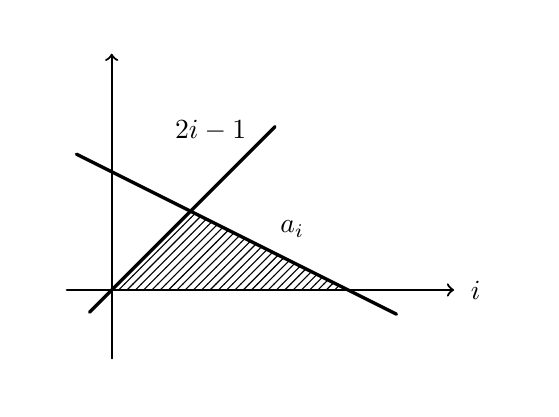
\begin{tikzpicture}[line cap=round,line join=round,x=1.0cm,y=1.0cm]
	\clip(-1.0672565565376129,-1.2619748573374914) rectangle (5.32499898604871,3.3308521813036203);
	\fill[line width=1.2pt,fill=black,pattern=north east lines,pattern color=black] (0.,0.) -- (3.,0.) -- (1.,1.) -- cycle;
	\draw (2.0174780216541786,1.000163833336489) node[anchor=north west] {$a_i$};
	\draw (0.6807597044377356,2.2854699075830687) node[anchor=north west] {$2i-1$};
	\draw [->,line width=0.8pt] (-0.5702715411622686,0.) -- (4.3481663696213095,0.);
	\draw [->,line width=0.8pt] (0.,-0.8678143279018735) -- (0.,3.);
	\draw (4.6223649987939135,0) node {$i$};
	\draw [line width=1.2pt] (-0.4482218066852332,1.7241109033426165)-- (3.6167728707986164,-0.30838643539930827);
	\draw [line width=1.2pt] (-0.28203886928823396,-0.28203886928823396)-- (2.074355600163829,2.074355600163829);
\end{tikzpicture}
\end{figure}
阴影部分面积可以近似看做求和的结果. 可以算出此时答案为$\fl{(n^2+n+1)/3}$. 我们可以证明如下:
\end{analysis}

\begin{solution}
\[\sum_{i=1}^{n}\min\{a_{i},2i+1\}\geq\left\{a_{1},a_{2},\cdots,a_{n},\{2i+1\}_{i=1}^n\right\}\text{中最小的}n\text{个数之和}=\fl{\frac{n^{2}+n+1}{3}}.\]
\end{solution}

\begin{example}
变量$ a_{1},a_{2},\cdots,a_{n}$满足$\{a_{1},a_{2},\cdots,a_{n}\}=\{1,2,\cdots,n\}$. 求
\[\sum_{i=1}^n\fl{\frac{a_i}{i}}\]
的最小值. 
\end{example}

\begin{analysis}
可以从较小的情况入手. \par
$n=3$: 不难发现最小值为
\[\fl{\frac{1}{1}}+\fl{\frac{3}{2}}+\fl{\frac{2}{3}}=2.\]\par 
$n=4$: 不难发现最小值为
\[\fl{\frac{1}{1}}+\fl{\frac{2}{2}}+\fl{\frac{4}{3}}+\fl{\frac{3}{4}}=3.\]\par
$n=5$: 不难发现最小值为
\[\fl{\frac{1}{1}}+\fl{\frac{2}{2}}+\fl{\frac{5}{3}}+\fl{\frac{3}{4}}+\fl{\frac{4}{5}}=3\]\par
$n=6$: 不难发现最小值为
\[\fl{\frac{1}{1}}+\fl{\frac{3}{2}}+\fl{\frac{2}{3}}+\fl{\frac{6}{4}}+\fl{\frac{4}{5}}+\fl{\frac{5}{6}}=3.\]\par
$n=7$: 不难发现最小值为
\[\fl{\frac{1}{1}}+\fl{\frac{3}{2}}+\fl{\frac{2}{3}}+\fl{\frac{7}{4}}+\fl{\frac{4}{5}}+\fl{\frac{5}{6}}+\fl{\frac{6}{7}}=3.\]\par
$n=8$: 不难发现最小值为
\[\fl{\frac{1}{1}}+\fl{\frac{2}{2}}+\fl{\frac{4}{3}}+\fl{\frac{3}{4}}+\fl{\frac{8}{5}}+\fl{\frac{5}{6}}+\fl{\frac{6}{7}}+\fl{\frac{7}{8}}=4.\]\par
如果读者亲自试着构造出了以上最小值, 大概会建立这样的直觉: 应当利用取整函数尽可能地“浪费”掉$a_i$. 比如说, 应当出现大量的$a_i=i-1$, 因为此时$\fl{a_i/i}=\fl{(i-1)/i}=0$, 这极大地“浪费”掉了$a_i$. 更次一点地, 对于那些不能保证$a_i=i-1$的$a_i$, 应当尽量保证$a_i=2i-1$或$a_i=2i-2$, 此时$\fl{a_i/i}=1$, 也“浪费”了很多.\par
为了更好地说明这一点, 我们可以取特例$n=2^m$. 对于$2^k<i\le 2^{k+1}\;(1\le k\le m-1)$, 可以取
\[a_{2^k+1}=2^{k+1}-1,a_{2^k+2}=2^k+1,a_{2^k+3}=2^k+2,\cdots,a_{2^{k+1}-1}=2^{k+1}-2,a_{2^{k+1}}=2^{k+1}-1.\]
这样做的好处, 就在于
\[\sum_{i=2^k+1}^{2^{k+1}}\fl{\frac{a_i}{i}}=\fl{\frac{2^{k+1}-1}{2^k+1}}+\fl{\frac{2^k+1}{2^k+2}}+\fl{\frac{2^k+2}{2^k+3}}+\cdots+\fl{\frac{2^{k+1}-2}{2^{k+1}-1}}+\fl{\frac{2^{k+1}-1}{2^{k+1}}}=1.\]\par 
整整$2^k$项的求和竟然只有$1$. 由此, 以及上面构造的$n=3,4,\cdots,8$的最小值, 可以猜测最小值为
\[1+\fl{\log_2 n}.\]\par
下面我们证明最小值确实是这样的. 提供两种证法, 一种基于偏组合的递归, 另一种基于一个局部不等式.
\end{analysis}

\begin{solution}
设$n$时的最小值为$x_n$. 我们利用递归的思想处理$x_n$(以下设$n\ge 3$): \par 
将$1$到$n$分为两部分: $A=\{1,2,\cdots,k\}$与$B=\{k+1,k+2,\cdots,n\}$, 其中$k=\fl{n/2}$. \note{这样划分的目的, 是为了找出$x_k$与$x_n$的关系; 在上文的构造中, 我们理应有$x_n\ge x_k+1$. 我们只\\需要找出一处$x_n$比$x_k$多的一处$1$即可. 于是, }考虑$n$的位置: 设$a_i=n$\note{显然$n$所在的分式更容易\\制造出我们想要的那个“$1$”}. 分类讨论:\par
(1) 若$i\in B$. 则
\[\sum_{i=1}^n\fl{\frac{a_i}{i}}=\sum_{i=1}^k\fl{\frac{a_i}{i}}+\sum_{i=k+1}^n\fl{\frac{a_i}{i}}\ge x_k+\fl{\frac{a_i}{i}}=x_k+1.\]
由此得$x_n\ge x_k+1$.\par
(2) 若$i\in A$. 则$i\le k$, $n-i\ge k$, 且
\[\fl{\frac{a_i}{i}}=\fl{\frac{n}{i}}=1+\fl{\frac{n-i}{i}}\ge 1+\fl{\frac{k}{i}}.\]
现在我们只考虑前半部分(即$j\in A$)中的项$a_j$. 将$a_j$中大于$k$项的分别减去一点, 不大于$k$的项不变, 使得
\[\{a_j':1\le j\le k\}=\{1,2,\cdots,k\}.\]
\note{上述操作的意义, 就是调整使得集合$\{a_i'\}_{i=1}^k$恰好等于$\{1,2,\cdots, k\}$, 从而对$a_1,\cdots,a_k$运用归纳\\假设. }其中$a_j'$为上述操作后的$a_j$. 则对任意的$j\in A\backslash\{i\}$, $a_j'\le a_j$, 故$\fl{a_j'/j}\le\fl{a_j/j}$; 而对于$i$,
\[\fl{\frac{a_i'}{i}}+1\le\fl{\frac{k}{i}}+1\le\fl{\frac{a_i}{i}}.\]
\note{上面的式子的含义是, 我们在$a_i$中找到了想要的那个“1”. }故
\[\sum_{j=1}^n\fl{\frac{a_j}{j}}\ge\sum_{j=1}^k\fl{\frac{a_j}{j}}=\fl{\frac{a_i}{i}}+\sum_{j\in A\backslash\{i\}}\fl{\frac{a_j}{j}}\ge1+\sum_{j=1}^k\fl{\frac{a_j'}{j}}\ge 1+x_k.\]
由此得$x_n\ge x_k+1$.\par
总之, 我们证明了, 对任意的$n\ge 3$, 有
\[x_n\ge x_{\fl{n/2}}+1.\]\par
由此, 结合$x_2=x_3=2$, 不难证明原命题成立. \par 
取等条件不难递归构造出: 取$a_1,a_2,\cdots,a_k$为$x_k$的取等, 再取
\[x_{k+1}=n,x_{k+2}=k+1,x_{k+3}=k+2,\cdots,x_{n}=n-1.\]
\end{solution}

\begin{solution}
我们证明一个局部不等式:
\[\fl{\frac{a_k}{k}}\ge\log_2{\frac{a_k+1}{k}}.\]\par
设$t=\fl{a_k/k}\in\mathbb{N}$. 则不难知道$t\ge\log_2{(t+1)}$. 而$t+1\ge (a_k+1)/k$, 故成立.\par
由上述不等式, 
\[\sum_{k=1}^n\fl{\frac{a_k}{k}}\ge\sum_{k=1}^n\log_2{\frac{a_k+1}{k}}=\sum_{k=1}^n\log_2{(a_k+1)}-\sum_{k=1}^n\log_2{k}=\log_2{(n+1)}.\]
结合整数的离散性知
\[\sum_{k=1}^n\fl{\frac{a_k}{k}}\ge\left\lceil\log_2{(n+1)}\right\rceil=\fl{\log_2n}+1.\]
\end{solution}

\begin{example}
变量$ a_{1},a_{2},\cdots,a_{n}$满足$\{a_{1},a_{2},\cdots,a_{n}\}=\{1,2,\cdots,n\}$. 求
\[f(a_1,a_2,\cdots,a_n)=a_1^{a_2^{\cdots^{a_n}}}\]
的最大值.
\end{example}

\begin{analysis}
为方便起见, 设
\[f(x_1,x_2)=x_1^{x_2},f(x_1,x_2,x_3)=x_1^{f(x_2,x_3)},\cdots,f(x_1,x_2,\cdots,x_k)=x_1^{f(x_2,x_3,\cdots,x_k)}.\]\par 
从小情况开始试验:\par 
(1) $n=3$, 显然最大值为$f(3,2,1)$;\par 
(2) $n=4$, 最大值为$f(2,3,4,1)$.\par
(3) $n=5$, 最大值为$f(2,3,4,5,1)$.\par
不难猜测一般情况下的最大值为$f(2,3,4,\cdots,n,1)$.
\end{analysis}

\begin{solution}
$n=3$时最大值为$f(3,2,1)$; 下设$n\ge 4$.
我们先证明一个引理(同时也是原命题的加强): 设$n\ge 3$, $\{y_1,y_{2},\ldots,y_{n}\}=\{x_{1},x_{2},\ldots,x_{n}\}$, 其中$2\leq x_{1}<x_{2}<\ldots<x_{n}$. 则有
\[f(y_1,y_2,\cdots,y_n)\le f(x_1,x_2,\cdots,x_n).\]
对$n$归纳证明:\par 
(1) $n=3$. 若$x_1=y_1$则显然成立. 若$y_1=x_2$, 则$f(y_1,y_2,y_3)=f(x_2,x_3,x_1)$或$f(x_2,x_1,x_3)$. 由$x_3\ge 4,x_1<x_3$知$x_1^{x_3}\ge x_3^{x_1}$, 故$f(x_2,x_3,x_1)\le f(x_2,x_1,x_3)$. 而求导不难得出
\[\frac{x_2^{x_3}}{\ln x_2}\ge\frac{x_1^{x_3}}{\ln x_1}\Rightarrow x_{2}^{x_{3}}\cdot\ln x_{1}\geq x_{1}^{x_{3}}\cdot\ln x_{2}\Rightarrow f(x_2,x_1,x_3)\le f(x_1,x_2,x_3).\]\par
若$y_1=x_3$. 运用完全相同的方法不难证明.\par
(2) 设命题在小于等于$n-1$时均成立, 考虑$n$的情况. 在原题中, 显然$a_n=1$, 否则将$a_n$与$1$所在的$a_i$互换, 表达式增大. 则此时可以忽略$1$, 加强命题. 设
\[\{a_{1},a_{2},\cdots,a_{n-1}\}=\{y_1,y_2,\cdots,y_{n-1}\}.\]\par
设$y_1=x_t$. 则由归纳假设, 有
\[f(y_1,\cdots,y_n)=y_1^{f(y_2,\cdots,y_n)}\le x_t^{f(x_1,\cdots,x_{t-1},x_{t+1},\cdots,x_n)}=f(x_t,x_1,\cdots,x_{t-1},x_{t+1},\cdots,x_n).\]
显然对于正整数$k\ge 2$, 函数$x^k/\ln(x)$在$\mathbb{N_+}$上是增函数, 故对正整数$a>b$, 有
\[\frac{a^k}{\ln a}\ge \frac{b^k}{\ln b} \Rightarrow (\ln b)\cdot a^k\ge (\ln a)\cdot b^k\Rightarrow b^{a^k}\ge a^{b^k}.\]
反复利用上述结论, 有
\begin{align*}
f(x_t,x_1,\cdots,x_{t-1},x_{t+1},\cdots,x_n)&\le f(x_1,x_t,x_2\cdots,x_{t-1},x_{t+1},\cdots,x_n)\\
&\le f(x_1,x_2,x_t,x_3,\cdots,x_{t-1},x_{t+1},\cdots,x_n)\\
&\le \cdots\\
&\le f(x_1,x_2,\cdots,x_{t-2},x_t,x_{t-1},x_{t+1},\cdots,x_n)\\
&\le f(x_1.x_2.\cdots.x_{t-1},x_{t},x_{t+1},\cdots,x_n).
\end{align*}
\end{solution}

\begin{example}
给定$n\in\mathbb{N}$.$ \{x_{1},x_{2},\ldots,x_{n}\}=\{1,2,\ldots,n\}$, 且$x_k\neq k\;(1\leq k\leq n)$. 求
\[\sum_{k=1}^{n}x_{k}k\]
的最大值.
\end{example}

\begin{analysis}
显然$x_k$尽量在$k$的附近最好. 即, 尽量做到$x_k\in\{k-1,k+1\}$. 结合$x_k\neq k$, 可以试着构造局部:
\[\left(x_k-(k-1)\right)\left(x_k-(k+1)\right)\ge 0 \Rightarrow kx_k\le\frac{x_k^2+k^2-1}{2}.\]
但$n$为奇数的时候不能取等(因为总有$k$使得$x_k\not\in\{k-1,k+1\}$). 我们应当提升放缩的精度, 取考虑更加细致的结构.\par 
$n$为偶数的时候可以取等:
\[(x_1,x_2,\cdots,x_n)=(2,1,4,3,\cdots,n,n-1).\]
$n$为奇数的时候, 可以猜测如下取等:
\[(x_1,x_2,\cdots,x_n)=(2,3,1,5,4,6,5,\cdots,n,n-1).\]
问题出现在$n$的奇偶性使得无法两两配对. 由此可以想到如下做法:
\end{analysis}

\begin{solution}
(1) $n$为偶数. 则
\[\sum_{k=1}^{n}kx_{k}\leq\sum_{k=1}^{n}\frac{k^2+x_{k}^2+1}{2}=\sum_{k=1}^{n}k^2-\frac{n}{2}=\frac{n(n+1)(2n+1)}{6}-\frac{n}{2}.\]\par
(2) $n$为奇数. 考虑有向图$G(V,E)$, $V=\{1,2,\cdots,n\}$, $E=\{(k,x_k):1\le k\le n\}$. 则$G$一定为若干个不交圈的并, 且一定存在某个圈的长度为奇数\note{我们在这里利用了$n$为奇数的条件; 这也是奇数和偶数情\\形的根本差别, 奇圈的长度不小于$3$, 这会带来更多的“损失”}. 取一个这样的圈, 其顶点集为$V_0$, 边集为$E_0$. 设$|G_0|=l\ge 3$. 设$d=\max\{V_0\}-\min\{V_0\}$, 则$d\ge l-1$. 则
\begin{align*}
\sum_{k=1}^{n}kx_{k}&=\sum_{(u,v)\in E_0}uv+\sum_{(u,v)\in E\backslash E_0}uv\\
&\le\sum_{(u,v)\in E_0}uv+ \sum_{(u,v)\in E\backslash E_0}\frac{u^2+v^2-1}{2}\text{\quad\note{这一步放缩与偶数情况相同}}\\
&=\sum_{(u,v)\in E_0}uv+\left(\sum_{u\in V\backslash V_0}u^2\right)-\frac{|V|-|V_0|}{2}\\
&=\sum_{(u,v)\in E_0}\frac{u^2+v^2-(u-v)^2}{2}+\left(\sum_{u\in V\backslash V_0}u^2\right)-\frac{n-l}{2}\text{\quad\note{这一步变形是为了像例1.1.2一样放缩}}\\
&=-\sum_{(u,v)\in E_0}\frac{(u-v)^2}{2}+\sum_{u\in V}u^2-\frac{n-l}{2}\\
&\le-\sum_{(u,v)\in E_0}\frac{3|u-v|-2}{2}+\frac{n(n+1)(2n+1)}{6}-\frac{n-l}{2}\text{\quad\note{这一步考虑了例1.1.2中的局部}}\\
&=-\frac{3}{2}\left(\sum_{(u,v)\in E_0}|u-v|\right)+l+\frac{n(n+1)(2n+1)}{6}-\frac{n-l}{2}\\
&\le -\frac{3}{2}\cdot 2d+\frac{n(n+1)(2n+1)}{6}+\frac{3l-n}{2}\\
&\le -\frac{3}{2}\cdot 2(l-1)+\frac{n(n+1)(2n+1)}{6}+\frac{3l-n}{2}\\
&\le \frac{n(n+1)(2n+1)}{6}-\frac{n+3}{2}.\text{\quad\note{因为$l\ge 3$}}
\end{align*}
故这种情况下有
\[\sum_{k=1}^{n}kx_{k}\le\frac{n(n+1)(2n+1)}{6}-\frac{n+3}{2}.\]
取等条件为
\[(x_1,x_2,\cdots,x_n)=(2,3,1,5,4,7,6,\cdots,n,n-1).\]
\end{solution}

\begin{example}
给定正整数$n$, 变量$\{x_1,x_2,\cdots,x_n\}=\{1,2,\cdots,n\}$, 求
\[\sum_{i=1}^{n} x_i^i\]
的最小值.
\end{example}

\begin{analysis}
显然, 若想取到最小值, 应当使$\{x_i\}$逆序排列. 即, 最小值应当为$\sum_{k=1}^n k^{n+1-k}$. \par 
对于这种问题, 通常采用\heiti{局部调整法}: 
\end{analysis}

\begin{solution}
考察如下局部调整: 若$a>b,c>d$, 则
\[a^c+b^d\ge a^d+b^c.\]
这等价于$a^c-a^d\ge b^c-b^d$. 而
\[a^c-a^d=a^d(a^{c-d}-1)\ge b^d(b^{c-d}-1)=b^c-b^d.\]\par
不断运用这个结论, 就能证明原问题.
\end{solution} 

通过前几个例题, 可以发现, 对于离散不等式有如下几个主要手段: \par 
\textbf{1. 局部不等式与整数离散性的应用}\quad 局部不等式一般是根据取等条件和式子结构而配制的. \par 
\textbf{2. “调整”思想}\quad “调整”思想有时可以指导我们进行正确的放缩. 即, 某些调整可以不明显地出现, 而隐藏在放缩中. 但必须注意调整的合理性.\par
\textbf{3. 通过归纳和加强命题化为更一般的问题}\quad 例如在例题1.3.5中, 原问题是不好使用归纳的. 将$\{1,2,\\ \cdots,n\}$换为更一般的$\{a_1,a_2\cdots,a_n\}$, 这样虽然加强了命题, 但更有利于归纳, 便于逻辑的顺畅.\par 
\textbf{4. 序列的具体性质}\quad 具体地研究离散数列的性质, 例如各种单调性、相邻项之间的差, 甚至各种组合性质(例如例题1.3.6)或是几何意义. 之后的章节会展示这样的思想.\par 

\begin{example}
给定正整数$n$. 实数$x_1,x_2,\cdots,x_n$满足$\{\fl{x_1},\fl{x_2},\cdots,\fl{x_n}\}=\{1,2,\cdots,n\}$. 求
\[\sum_{i=1}^{n-1}\fl{x_{i+1}-x_i}\]
的最大值与最小值.
\end{example}

\begin{solution}
由$\fl{a+b}\ge\fl{a}+\fl{b}$知$\fl{a-b}\le\fl{a}-\fl{b}$. 故
\[\sum_{i=1}^{n-1}\fl{x_{i+1}-x_i}\le \fl{x_n}-\fl{x_1}\le n-1.\]\par 
故最大值为$n-1$, $x_i=i$时取等.\par 
而由$\fl{a}>a-1$知$\fl{x_{i+1}-x_i}\ge x_{i+1}-x_i-1$, 故
\[\sum_{i=1}^{n-1}\fl{x_{i+1}-x_i}> -n+1+x_n-x_1> -2n+1.\]
结合整数的离散性得
\[\sum_{i=1}^{n-1}\fl{x_{i+1}-x_i}\ge -2n+2.\]\par
取等: $x_k=(n+2)(n+1-k)/(n+1).$
\end{solution}

下面介绍一个与数论和组合相关的问题.

\begin{example}
$a_1,a_2,\cdots,a_{17}$为$1,2,\cdots,17$的一个排列, 且存在正整数$n$满足
\[\prod_{i=1}^{17}(a_{i+1}-a_i)=n^{17}.\]
其中$a_{18}=a_1$. 求$n$的最大可能值.
\end{example}

\begin{analysis}
先对式子进行放缩:
\[n^{17}=\prod_{i=1}^{17}(a_{i+1}-a_i)\le\left(\frac{1}{17}\sum_{i=1}^{17}|a_i-a_{i+1}|\right)\Rightarrow 17n\le\sum_{i=1}^{17}|a_i-a_{i+1}|\]\par 
于是问题转向了估计$\sum_{i=1}^{17}|a_i-a_{i+1}|$的最大值. 常见的手法是
\begin{align*}
\sum_{i=1}^{17}|a_i-a_{i+1}|&=\sum_{i=1}^{17}\left(a_i+a_{i+1}-2\min\{a_i,a_{i+!}\}\right)=17\cdot 18-2\sum_{i=1}^{17}\min\{a_i,a_{i+1}\}\\
&\le 17\cdot 18-2(1+1+2+2+\cdots+8+8+9)\text{\note{此即$1,1,2,2,\cdots,17,17$中较小的17个数}}\\
&=144.
\end{align*}
由此便可以得到$n\le 8$. \par 
为了给出具体构造, 我们不得不考虑数论性质. 若$n=7$或$8$, 注意到$7$和$8$各只有一种素因子, 存在对应的构造的可能性不是很大, 动手试验之后发现的确如此. 对于$n=6$, 由于素因子有两种($2$和$3$), 故构造的灵活性更大($|a_{i+1}-a_i|$可以等于$1,2,3,4,6,8,9,12,16$), 更容易构造出相应的取等条件.
\end{analysis}

\begin{solution}
由上文知$n\le 8$. 若$n=8$, 则
\[51=v_2(n^{17})=\sum_{i=1}^{17}v_2(|a_{i+1}-a_i|).\]
其中$v_p(m)$表示$m$中$p$的幂次($p$为素数). 注意到最多存在一个$i$使得$v_2(|a_{i+1}-a_i|)=4$, 对于其余的$i$均有$v_2(|a_{i+1}-a_i|)\le 3$; 并且至少存在一个$j$使得$v_2(|a_{j+1}-a_j|)=0$, 即$|a_{j+1}-a_j|$为奇数. 故
\[\sum_{i=1}^{17}v_2(|a_{i+1}-a_i|)\le 4+3\cdot 15<51.\]
故$n\neq 8$. 若$n=7$, 则
\[\sum_{i=1}^{17}v_7(|a_{i+1}-a_i|)=17.\]
这是不可能的, 因为对于任意的$i$均有$v_7(|a_{i+1}-a_i|)\le 1$并且至少存在一个$i$使得$v_7(|a_{i+1}-a_i|)=0$, 即$|a_{i+1}-a_i|$不是$7$的倍数.\par 
故$n\le 6$. 下面给出$n=6$的构造:
\[1,10,2,11,3,12,15,6,4,13,5,14,16,7,8,17,9.\]
\end{solution}

\begin{example}
给定正整数$n\ge 2$. 变量$a_1,a_2,\cdots,a_n;b_1,b_2,\cdots,b_n$满足$\{a_1,a_2,\cdots,a_n,b_1,b_2,\cdots,b_n\}=\{1,2,\cdots,2n\}$. 对于$1\le i\le n$, 记$c_i=a_ib_i$; $c_{n+1}=c_1$. 求
\[\sum_{i=1}^n|c_i-c_{i+1}|\]
的最小值.
\end{example}

\begin{analysis}
看到这个问题, 不难注意到以下要点: \par 
首先, $\sum_{i=1}^n|c_i-c_{i+1}|$在某种程度上刻画了数组$\{c_i\}$的“分散程度”. 即, 若想求得最小值, 那么必须让数组$\{c_i\}$相对而言最集中. 由此, 不难想到取等: $a_k=k,b_k=2n+1-k\;(1\le k\le n)$.\par 
其次, 我们已经见了不止一次类似于$\sum_{i=1}^n|c_i-c_{i+1}|$的式子了. 由于在本题中, 我们可以{\heiti 随意调换各$c_i$的排列方式}而不产生任何矛盾, 故可以直接做放缩: 
\[\sum_{i=1}^n|c_i-c_{i+1}|\ge 2\left(\max\limits_{1\le i\le n}c_i-\min\limits_{1\le i\le n}c_i\right).\]\par 
因此, 我们只需关注数组$\{c_i\}$的极差. 设
\[c_j=\max\limits_{1\le i\le n}c_i,\;c_k=\min\limits_{1\le i\le n}c_i.\]
在我们构造出的取等中, $c_j=n(n+1),\;c_k=2n$. 我们采取下面的方法说明$c_j-c_k$的最小值, 即说明$c_j$不小于某个数(在本题中是$n(n+1)$), 同时$c_k$不大于某个数(在本题中是$2n$). 具体方法如下.
\end{analysis}

\begin{solution}
一方面, 取$a_k=k,b_k=2n+1-k\;(1\le k\le n)$, 知此时
\[\sum_{i=1}^n|c_i-c_{i+1}|=2n(n-1).\]
下面证明最小值为$2n(n-1)$. 设
\[c_j=\max\limits_{1\le i\le n}c_i,\;c_k=\min\limits_{1\le i\le n}c_i.\]
则
\[\sum_{i=1}^n|c_i-c_{i+1}|\ge 2\left(\max\limits_{1\le i\le n}c_i-\min\limits_{1\le i\le n}c_i\right)=2(c_j-c_k).\]\par 
下面我们证明$c_j\ge n(n+1),\; c_k\le 2n$(从而$c_j-c_k\ge n(n-1)$, 原不等式得证.)\par 
设下标$u$使得$a_u=1$或$b_u=1$, 则又$a_u\le 2n,\; b_u\le 2n$, 知
\[c_k\le c_u=a_ub_u\le 2n\cdot 1=2n.\]
下证$c_j\ge n(n-1)$. \note{为了更好地刻画$\{a_i\}$与$\{b_i\}$的关联, 我们}构造图$G(V,E)$, 其中$V=\{1,2,\cdots,2n\}$, $E=\{\{a_i,b_i\}:1\le i\le n\}$. 取$V_1=\{1,2,\cdots,n-1\},\;V_2=V\backslash V_1.$\par 
显然, 图$G$中的边两两不交. 若$V_2$中没有顶点相连, 则所有的边都在$V_1$中占据至少一个顶点, 即此时有$|V_1|\ge|E|$. 而这显然是不成立的. \note{直观上来说, $V_1$“太小了”以至于无法“放得下”\\所有的边, 所以一定有的边被迫“挤出”$V_1$而到$V_2$中. }故$V_2$中一定有顶点相连, 设此边为$\{a_v,b_v\}$. 则$a_v\ge n,b_v\ge n$且$a_v\neq b_v$, 故
\[c_j\ge c_v=a_vb_v\ge n(n+1).\]\par 
故$c_j\ge n(n+1),\; c_k\le 2n$, 从而原命题得证.
\end{solution}

\begin{example}
给定正整数$m,n,k\ge2,n>k$, 考虑在一个$m$行$n$列的方格表中填入$1,2,\dots{},mn$, 满足每一行填入的数从左到右单调递增, 求该方格从左往右数表前$k$列中填入的数之和的最大可能值.
\end{example}
\begin{analysis}
我们先分析从左到右单调递增与前$k$列带给我们的感受, 那么这表明每行参与求和的是最小的$k$个数, 因为要求最大值, 我们自然地考虑这些参与求和的数中最大的数可能是多少. 事实上, 一定不超过$mn-n+k$, 因为整个方格表中一定还有$n-k$个更大的数, 如果取到这个值, 那么剩下的数从大到小排分别不超过$mn-n+k-1,mn-n+k-2,\dots{}$, 并且, 如果后面依次将这些数全部取到, 那么再往后的数便要从$mn-2n+k$加起. 这样下去, 我们大概有了一个初步的感受, 考虑如下构造: 
\begin{center}
第$l$行$(1\le l\le m)$为$ln-n+1,ln-n+2,\dots{},ln$
\end{center}

进一步, 在证明中, 按照这个思路, 我们便发现第$kt-k+1$到$kt$大的数中, 这些数是比较有特点的, 是取等中第$t$列的前$k$个数, 我们便想到可以考虑从第$kt$大的数处将这些数截断, 去考察第$kt-k+1$到$kt$大的数之和的放缩, 其实也只需考虑第$kt$大的数的放缩.
\end{analysis}

\begin{solution}
一方面, 按照分析中的构造, 我们算出该和为
\[\frac{knm(m-1)+k(k+1)m}{2}.\]

另一方面, 下考虑证明, 只需证对$1\le t\le m$, 这些加数中第$kt-k+1$到$kt$大的数之和不超过
\[
\sum_{s=1}^k ((t-1)n+s).
\]

由于这些数两两不同, 这只需第$kt$大的数不超过$(t-1)n+k$, 设这个数为$r$

我们将$1,2,\dots{},r$重新按从小到大填入这个表格中, 并且将已经填入的数标红\note{这样便于我们\\去刻画
“第$kt$大”}, 则$r$为红数的个数. 在第$k$列(含)左边, 红数一共$kt$个, 考察第$k$列(不含)右边的总红格数, 将第$k$列(不含)右边出现红格的行称为“好行”\note{这是去考察红格总数的必要一步, 剩下的步骤便都较为自然了}.

如果一个行为“好行”, 那么在这个行的前$k$列中, 一定都是红格, 否则与每行填入的数单调递增矛盾, 同时, 由于$r$是最后填入的数, 且在第$k$列(含)左边, 故$r$所在行不为好行, 因此, 全体好行在第$k$列(含)左边一共有不超过$kt-1$个数, 故好行不超过$t-1$个.

考察所有的好行, 其中每行在第$k$列(不含)右边出现红格不超过$n-k$个, 因此红格个数一共不超过
\[
(t-1)(n-k)+tk=(t-1)n+k.
\]

因此, $r\le (t-1)n+k$, 这样我们便完成了证明.
\end{solution}



\exercisetitle

\begin{exercise}
使用归纳法证明例题1.1.2, 甚至例题1.1.1.
\end{exercise}

\begin{exercise}
变量$a_1,\cdots,a_{10}$满足$\{a_1,\cdots,a_{10}\}=\{1,2,\cdots,10\}$. 求$\sum_{i=1}^9 a_i^2 a_{i+1}$的最小值与最大值.
\end{exercise}

\begin{exercise}
$a_1,a_2,\cdots,a_{17}$为$1,2,\cdots,17$的一个排列, 且存在正整数$n$满足
\[\prod_{i=1}^{17}(a_{i+1}-a_i)=2^n.\]
其中$a_{18}=a_1$. 求$n$的最大可能值.
\end{exercise}

\begin{exercise}
变量$a_1,\cdots,a_{20}$满足$\{a_1,\cdots,a_{20}\}=\{1,2,\cdots,20\}$. 记
\[M=\max\limits_{1\le k\le 20}|a_k-a_{k+1}|,\;m=\min\limits_{1\le k\le 20}|a_k-a_{k+1}|.\]
求$m\cdot M$的最小值与最大值.
\end{exercise}

\begin{exercise}
变量$a_1,a_2,\cdots,a_{101}$满足$\{a_{1},a_{2},\cdots,a_{101}\}=\{1,2,\cdots,101\}$. 求
\[\sum_{k=1}^{101}(\mathrm{lcm}(a_{k},k))^{\frac{3}{2}}\]
的最大值.
\end{exercise}

\begin{exercise}
变量$a_1,\cdots,a_{100};b_1,\cdots,b_{100}$满足$\{a_1,a_2,\cdots,a_{100}\}=\{b_1,b_2,\cdots,b_{100}\}=\{1,2,\cdots,100\}$. 求
\[M=\max_{1\leq k\leq100}\{ka_{k}b_{k}\}\]
的最小值.
\end{exercise}

\begin{exercise}
给定正整数$n\ge 4$, 将$1,2,\dots{},n^2$填入一个$n\times n$的方格表, 考虑所有有公共边的两个格子中的数的和, 考虑这些和中最大的记作$M$, 求$M$的最小可能值.
\end{exercise}


\section{整数离散性以及经典方法}

为了获得更好的阅读体验, 建议读者掌握以下预备知识:\par 
\textbf{1. 整数离散性的各种应用}\quad 这已经在前面的例题中初步学习.\par 
\textbf{2. Karamata不等式}\quad 设函数$f(x)$在$[a,b]$上连续, 在$(a,b)$上二阶可导且$f''(x)\ge 0$对$\forall x\in (a,b)$成立. 此时称$f$为下凸函数. 若$f''\le 0$则称为上凸函数\footnote{有些参考书籍上将上凸函数称为凹函数, 将下凸函数称为凸函数; 更有甚者将上凸函数称为凸函数而将下凸函数称为凹函数; 还有的书使用“上凹”和“下凹”的术语; 总之, 有关凹凸性的术语较为混乱. 我们呼吁大家使用标准、直观且不易出错的“上凸”和“下凸”的术语.}. 对于数列$\{a_i\}_{i=1}^{n}$与$\{b_i\}_{i=1}^{n}$, 若$a_1\ge a_2\ge\cdots\ge a_n$, $b_1\ge b_2\ge\cdots\ge b_n$, 且
\[\sum_{i=1}^{n}a_i=\sum_{i=1}^{n}b_i;\;\forall1\leq j\leq n-1, \sum_{i=1}^{j}a_{i}\ge\sum_{i=1}^{j}b_{i},\]
则称$\{a_i\}$优超于$\{b_i\}$, 记作$\{a_i\}\succ\{b_i\}$. \par
Karamata不等式, 即对于$(a,b)$上的下凸函数$f(x)$以及数列$\{a_i\}_{i=1}^{n}$与$\{b_i\}_{i=1}^{n}$, 其中$\{a_i\}\succ\{b_i\}$, 则
\[\sum_{k=1}^{n}f(a_k)\ge\sum_{k=1}^{n}f(b_k).\]
对于上凸函数也有类似结论. 下面证明这个不等式, 使用Abel变换:\par 
\begin{align*}
\sum_{k=1}^{n}(f(b_{k})-f(a_{k}))&=\sum_{k=1}^{n}\frac{f(b_{k})-f(a_{k})}{b_{k}-a_{k}}(b_{k}-a_{k})\\
&=\sum_{k=1}^{n}\left(\frac{f(b_{k})-f(a_{k})}{b_{k}-a_{k}}-\frac{f(b_{k-1})-f(a_{k-1})}{b_{k-1}-a_{k-1}}\right)\left(\sum_{j=1}^{k}(b_{j}-a_{j})\right)\le 0.
\end{align*}
其中, 由下凸函数的性质, 有
\[\frac{f(b_{k})-f(a_{k})}{b_{k}-a_{k}}\ge\frac{f(b_{k-1})-f(a_{k})}{b_{k-1}-a_{k}}\ge \frac{f(b_{k-1})-f(a_{k-1})}{b_{k-1}-a_{k-1}}.\]\par 
\textbf{3. 各种代数变形}\quad 例如著名的Abel变换: $\{a_i\}_{i=1}^{n}$与$\{b_i\}_{i=1}^{n}$为两组数列, 记$S_k=\sum_{i=1}^{k}a_i$, 则有
\[\sum_{i=1}^{n}a_ib_i=S_nb_n+\sum_{i=1}^{n-1}S_i(b_i-b_{i+1}).\]
此变换的主要功效是, 对于两个数列的对应项乘积的和$\sum_{i=1}^{n}a_ib_i$, Abel变换可以将此和对应为其中一个数列的部分和(即$S_i$)与另一个数列的差分(即$b_i-b_{i+1}$)的对应项乘积的和. 在一些时候, 使用部分和会得到很奇妙的结果. 

先给出几道例题将展示处理最大公约数, 最小公倍数的方法.

\begin{example}
给定正整数$t>1$, 对于整数序列$a_0,a_1,a_2,\cdots,a_n,\cdots$, 满足对$i\ge 1$, 有$(a_i,a_{i+1})> (t-1)a_{i-1}$. 求证: $a_n\ge t^n$.
\end{example}

\begin{analysis}
自然地分析, 如果$x>y$, 我们一般可以得到$x\ge y+1$, 但是在这里, 注意到取等$a_{n}=t^n$, 此时, 仅仅使用$(a_i,a_{i+1})\ge (t-1)a_{i-1}+1$似乎就不够了, 这里我们希望加的是一个类似$t^{i-1}$的数. \par
我们重新审视$x>y$推出的结论, 如果我们真的想让$x\ge y+k$, 有没有一个较好的$k$的形式呢?事实上, 直接使用整数离散型并不能得到什么结果, 但如果联想该不等式的取等, 例如加上条件$t|x,y$, 那么我们显然有$x\ge x+t$, 所以自然地, 我们会想到放缩$x\ge y+\gcd{(x,y)}$, 这样, 我们便获得了一个思路, 使用$(a_i,a_{i+1})\ge (t-1)a_{i-1}+(a_{i-1},a_i,a_{i+1})$.

接下来, 我们考虑$(a_{i-1},a_i,a_{i+1})$的放缩, 事实上, 形式驱使我们往$(a_i,a_{i+1})$这样的结构去放缩, 因此我们可以构建不等式$x(x,y,z)\ge (x,y)(x,z)$, 剩余的部分便是自然的了.

我们给出两种解法, 其中第一种是基于分析的解法.
\end{analysis}



\begin{solution}
先证明一个引理: 
\begin{lemma}
对正整数$x,y,z$, 有$x(x,y,z)\ge (x,y)(x,z)$.
\end{lemma}

这是因为, 不妨设$(x,y,z)=1$, 则$((x,y),(x,z))=1$, 于是$(x,y)(x,z)|x$, 即$x(x,y,z)\ge (x,y)(x,z)$, 即证.

回原题. 于是有
\[
(a_i,a_{i+1})\ge (t-1)a_{i-1}+(a_{i-1},a_i,a_{i+1})\ge (t-1)a_{i-1}+\frac{(a_{i-1},a_i)(a_i,a_{i+1})}{a_{i}}\ge t\sqrt{\frac{a_{i-1}(a_{i-1},a_i)(a_i,a_{i+1})}{a_{i}}}.
\]

整理得
\[
a_{i}(a_i,a_{i+1})\ge t^2 a_{i-1}(a_{i-1},a_i) \ge \dots{} \ge t^{2i}a_0(a_0,a_1).
\]

因此$a_n\ge \sqrt{a_n(a_n,a_{n+1})}\ge t^n$, 命题得证.
\end{solution}

\begin{solution}
设
\[\frac{a_{i+1}}{a_{i}}=\frac{x_{i}}{y_{i}},(x_{i},y_{i})=1.\]
这样, 就有
\[(a_{i},a_{i+1})=(a_{i},a_{i}\cdot\frac{x_{i}}{y_{i}})=\frac{a_{i}}{y_{i}}.\]
结合条件, 有$a_i/{y_i}>a_{i-1}$. 由此得$ c{x_{i-1}}/{y_{i-1}}={a_{i}}/{a_{i-1}}>y_{i}$, 即
\[\frac{x_{i-1}}{y_{i-1}}>y_{i}.\]
再结合整数的离散性, 得$x_{i-1}\geq y_iy_{i-1}+1$, 故
\[\frac{x_{i-1}}{y_{i-1}}\ge (t-1)y_i+\frac{1}{y_{i-1}}\ge t\sqrt{\frac{y_i}{y_{i-1}}}.\]
将这个式子对$i$累乘, 有
\begin{align*}
a_{n}&=\frac{x_{n-1}}{y_{n-1}}\cdot\frac{x_{n-1}}{y_{n-1}}\cdots\cdot\frac{x_{n}}{y_{n}}\cdot y_{n}\geq t\sqrt{\frac{y_{n}}{y_{n-1}}}\cdot t\sqrt{\frac{y_{n-1}}{y_{n-2}}}\cdots\cdot t\sqrt{\frac{y_{1}}{y_{n}}}\cdot y_{0}\\
&=t^{n}\sqrt{y_{n}y_0}\geq t^{n}.
\end{align*}
\end{solution}


\begin{example}
给定正整数$m,n$, 满足$n\ge 3m$. 对于
\[\sum_{k=1}^{n}x_{k}=m(2n-1) \quad (x_{k}\in \mathbb{N}^+),\]
求
\[ \sum_{k=1}^{n}\gcd(x_{k},x_{k+1},x_{k+2}) \]
的最大值. (下标模$n$理解)
\end{example}

\begin{analysis}
不难猜到一个取等, 即
\[x_1=m,x_2=x_3=\cdots=x_n=2m.\]
此时答案为$m(2n-3)$.\par 
为了化简问题, 设$d_i=(x_i=x_{i+1})$. 这样, 由于$(x_i,x_{i+1},x_{i+2})\le (d_i,d_{i+1})$, 就可以先求出$\sum_{i=1}^nd_i$的上界, 进而求出原式的上界.\par 
注意到取等时很多的$x_i$都相等, 故可以先考虑使$x_i\neq x_{i+1}$的$x_i$, 此时$d_i=(x_i,x_{i+1})$通常会有一个不错的上界.
\end{analysis}

\begin{solution}
先证明$\sum_{i=1}^nd_i\le m(2n-2)$:\par
由$n\not|\;m(2n-1)$知存在$i$使得$x_i\neq x_{i+1}$. 不妨设$x_{i}>x_{i+1}$. 则
\[\sum_{k=1}^{n}d_{k}=\left(\sum_{k\neq i,i+1}x_{k}\right)+x_{i}-x_{i+1}+x_{i+1}=\left(\sum_{k=1}^{n}x_{k}\right)-x_{i+1}=m(2n-1)-x_{i+1}.\]
故若$x_{i+1}\ge m$则得证; 下设$x_{i+1}\ge m-1$.\par 
先提出一个有用的引理: 
\begin{lemma}
对任意的实数$y_1,y_2,\cdots,y_n$, 均有
\[\sum_{k=1}^{n-1}\min\{y_{k},y_{k+1}\}\leq\frac{n-1}{n}\sum_{k=1}^{n}y_{k}.\]
\end{lemma}
这是因为: 
\[\sum_{k=1}^{n-1}\min\{y_{k},y_{k+1}\}\leq\sum_{k=1}^{n-1}\left(\frac{n-k}{n}y_{k}+\frac{k}{n}y_{k+1}\right)=\frac{n-1}{n}\sum_{k=1}^{n}y_{k}.\]
回原题, 于是有
\[\sum_{k\neq i,i+1}\min\{x_{k},x_{k}\}\leq\frac{n-2}{n-1}\left(\sum_{k\neq i+1}x_{k}\right)=\frac{n-2}{n-1}(m(2n-1)-x_{i+1}).\]
故
\[\sum_{k=1}^{n}d_{k}=d_i+d_{i+1}+\sum_{k\neq i,i+1}\min\{x_{k},x_{k}\}\le 2x_{i+1}+\frac{n-2}{n-1}(m(2n-1)-x_{i+1})\le m(2n-2).\]\par 
再证明$\sum_{i=1}^{n}(d_{i},d_{i+1})\le m(2n-3)$.\par 
\note{若想沿用上面的做法, 必须找出$d_{i}\neq d_{i+1}$, 故必须先讨论}若$d_1=d_2=\cdots=d_n=d$. 则
\[ \sum_{i=1}^{n}(d_{i},d_{i+1})=nd. \]
设$y_k=dx_k$, 则$(x_k,x_{k+1})=1$, 且$d\cdot\left(\sum_{i=1}^n y_i\right)=m(2n-2)$. 显然有$\sum_{i=1}^{k}y_k\ge n+1$(因为$x_i$不能全相同, 所以$y_i$也不能全都为$1$).\par 
若$\sum_{i=1}^{k}y_k=n+1$, 则有
\[n+1|m(2n-1)\Rightarrow n+1|m(3(n+1)-(2n-1))\Rightarrow n+1|3m\Rightarrow n<3m.\]
矛盾!\par 
若$\sum_{i=1}^{k}y_k\ge n+2$, 则
\[nd=n\cdot\frac{m(2n-2)}{\sum_{i=1}^{k}y_k}\le m\frac{n(2n-2)}{n+2}\le m(2n-3).\quad\text{(因为$n\ge 3$)}\]
此时原命题成立. \par 
反之, 若$d_i$不全相等, 取$d_i\neq d_{i+1}$, 并不妨设$d_i>d_{i+1}$.\par 
若$d_{i+1}\ge m$, 与第一部分完全类似地, 有
\[\sum_{k=1}^{n}(d_{k},d_{k+1})=\left(\sum_{k\neq i,i+1}d_{k}\right)+d_{i}-d_{i+1}+d_{i+1}=\left(\sum_{k=1}^{n}d_{k}\right)-d_{i+1}=m(2n-2)-d_{i+1}\le m(2n-3).\]
若$d_{i+1}\le m-1$, 则同样与第一部分完全类似地, 有
\begin{align*}\sum_{k=1}^{n}(d_{k},d_{k+1})
&\leq\sum_{k=1}^{n}\min\{d_{k},d_{k+1}\}\leq2d_{i+1}+\sum_{k\neq i}\min\{d_{i},d_{i+1}\}\\
&\leq2d_{i+1}+\frac{n-2}{n-1}(m(2n-2)-d_{i+1})\leq\frac{(m-1)n}{n-1}+\frac{n-2}{n-1}m(2n-2)\\
&=\frac{(m-1)n+m(n-2)(2n-2)}{n-1}\\
&=\frac{m(2n^{2}-6n+4+n)-n}{n-1}=\frac{m(2n^{2}-5n+3)+m-n}{n-1}\\
&=\frac{m(n-1)(2n-3)}{n-1}+\frac{m-n}{n-1}=m(2n-1)+\frac{m-n}{n-1}\\
&<m(n-3)
\end{align*}
故
\[\sum_{k=1}^{n}(x_{k},x_{k+1},x_{k+2})\le\sum_{i=1}^{n}(d_{i},d_{i+1})\le m(2n-3).\]
\end{solution}

\begin{example}
求最小的常数$C$, 使得对任意严格递增的正整数序列$a_1<a_2<\cdots<a_n$, 均有($a_{n+1}=a_1$)
\[\sum_{k=1}^{n}\frac{1}{[a_{k},a_{k+1}]}\leq C.\]
\end{example}

\begin{analysis}
对于两个整数的最小公倍数的倒数, 有一个不错的估计:
\[\frac{1}{[a,b]}=\frac{(a,b)}{ab}\le\frac{|a-b|}{ab}=\left|\frac{1}{a}-\frac{1}{b}\right|.\]
这样的好处是, 若$a$和$b$的大小关系给定, 那么这个不等式提供了一个裂项. 取等条件当然是$|a-b|=(a,b)$.
\end{analysis}

\begin{solution}
\[\sum_{k=1}^{n}\frac{1}{[a_{k},a_{k+1}]}=\frac{1}{[a_1,a_n]}+\sum_{k=1}^{n-1}\frac{1}{[a_{k},a_{k+1}]}\le \frac{1}{a_n}+\sum_{k=1}^{n-1}\left(\frac{1}{a_k}-\frac{1}{a_{k+1}}\right)=\frac{1}{a_1}\le 1.\]
另一方面, 取$a_i=2^{i-1}$, 知此时原式为$1$. 故$C$的最小值为$1$.
\end{solution}

在上面展示的最大公约数与最小公倍数的问题中, 我们主要使用了一些\textbf{数论性质以及整数离散性}, 同时, 基于\textbf{莫比乌斯反演}, 我们可以得到一些离散不等式, 尤其涉及到整除的数论性质的问题的奇妙做法, 先看一个定理.

\begin{theorem}
\[n=\sum_{d|n}\varphi (d).\]
\end{theorem}

这个定理的证明我们不予给出, 参见《数论: 概念与问题》; 接下来我们通过几个例题来展示它的妙用: 

\begin{example}
给定正整数$n>2$与正实数$\lambda$, 正整数$a_1,a_2,\dots{},a_n,b_1,b_2,\dots{},b_n$满足对任意$1\le k\le n,1\le i_1<i_2<\dots{}<i_k\le n$, 均存在$1\le j_1<j_2<\dots{}<j_k\le n$, 满足$\gcd{(a_{i_1},a_{i_2},\dots{},a_{i_k})}$整除$\gcd{(b_{j_1},b_{j_2},\dots{},b_{j_k})}$, 证明: 
\[
\sum_{k=1}^n a_k^{\lambda}\le \sum_{k=1}^n b_k^{\lambda}.
\]
\end{example}

\begin{analysis}
首先去理解条件: 对任意$1\le k\le n,1\le i_1<i_2<\dots{}<i_k\le n$, 均存在$1\le j_1<j_2<\dots{}<j_k\le n$, 满足$\gcd{(a_{i_1},a_{i_2},\dots{},a_{i_k})}|\gcd{(b_{j_1},b_{j_2},\dots{},b_{j_k})}$, 

从字面上来讲, 这似乎说明了序列$\{b_i\}$在因子上优于$\{a_i\}$, 在这个感受下, 我们看看对任意正整数$d$, 两个序列被$d$整除的数有怎样的关系, 首先, 如果$d|\gcd{(a_{i_1},a_{i_2},\dots{},a_{i_k})}$, 那么一定存在$1\le j_1<j_2<\dots{}<j_k\le n$使得$d|\gcd{(b_{j_1},b_{j_2},\dots{},b_{j_k})}$, 我们让这样的$a_{i_j}$最多, 也就是取出所有的被$d$整除的$\{a_i\}$中的项放在左边, 那么这表明$d$整除的$\{a_i\}$中的项数不大于$d$整除的$\{b_i\}$中的项数; 

另一方面, 这也驱使我们考察这是否是充要条件, 如果$d$整除的$\{a_i\}$中的项数大于$d$整除的$\{b_i\}$中的项数, 这明显导致了一个矛盾, 我们设$1\le i_1<i_2<\dots{}<i_k\le n$是全体被$d$整除的$\{a_i\}$中的项的下标, 于是对任意$1\le j_1<j_2<\dots{}<j_k\le n$, $d$不能整除$\gcd{(b_{j_1},b_{j_2},\dots{},b_{j_k})}$, 这会导致矛盾.

在等价转换后, 命题便变得清晰, 我们的条件是对任意正整数$d$, $d$整除的$\{a_i\}$中的项数不大于$d$整除的$\{b_i\}$中的项数, 于是我们需要考察证明式中的式子是否能用这些量表示, 使用定理类似的内容, 问题便迎刃而解.
\end{analysis}

\begin{solution}
若存在正整数$d$, 使得$d$整除的$\{a_i\}$中的项数大于$d$整除的$\{b_i\}$中的项数, 那么设$1\le i_1<i_2<\dots{}<i_k\le n$是全体被$d$整除的$\{a_i\}$中的项的下标, 于是对任意$1\le j_1<j_2<\dots{}<j_k\le n$, $d$不能整除$\gcd{(b_{j_1},b_{j_2},\dots{},b_{j_k})}$, 与条件矛盾!

于是对任意正整数$d$, $d$整除的$\{a_i\}$中的项数不大于$d$整除的$\{b_i\}$中的项数.

对正整数$n=\prod_{k=1}^r p_{j}^{\alpha_j}$, 定义
\[u(n)=\prod\limits_{k=1}^r p_{j}^{\lambda\alpha_j-\lambda}(p_j^{\lambda}-1).\]

对正整数$d$定义$f(d),g(d)$分别是$d$整除$\{a_i\}$与$\{b_i\}$中的项数, \note{类似于上面给出的定理, }我们有
\[
m^{\lambda}=\sum_{d|m}u(d)=\sum_{d=1}^{\infty} \mathbf{1}_{d|m}u(d).
\]

于是就有: 
\[
\sum_{k=1}^n a_k^{\lambda}=\sum_{k=1}^n \sum_{d=1}^{\infty} \mathbf{1}_{d|a_k}u(d)=\sum_{d=1}^{\infty}u(d)\sum_{k=1}^n\mathbf{1}_{d|a_k}=\sum_{d=1}^{\infty}u(d)f(d).
\]

条件即为对任意正整数$d$, $f(d)\le g(d)$, 于是
\[
\sum_{k=1}^n a_k^{\lambda}=\sum_{d=1}^{\infty}u(d)f(d)\le \sum_{d=1}^{\infty}u(d)g(d) =\sum_{k=1}^n b_k^{\lambda}.
\]

命题得证.
\end{solution}

\begin{example}
给定正整数$n>m$, 求最小的正实数$\lambda$, 使得对任意$n$个正整数$x_1,x_2,\dots{},x_n$, 均有
\[
\sum_{k=1}^nx_k-\sum_{k=1}^n{(x_i,x_{i+1},\dots{},x_{i+m})}\le \lambda ({[x_1,x_2,\dots{},x_n]}-{(x_1,x_2,\dots{},x_n)}).
\]

其中, 下标$\mathrm{mod}\ n$理解.
\end{example}

\begin{analysis}
这个问题要介绍定理$1.4.1$在最大公约数中的妙用, 我们使用定理$1.4.1$, 于是有
\[
(x_1,x_2,\dots{},x_n)=\sum_{d=1}^{\infty} \varphi(d)\mathbf{1}_{d|x_1,x_2,\dots{},x_n}=\sum_{d=1}^{\infty} \varphi(d)\prod_{k=1}^n \mathbf{1}_{d|x_k}.
\]

这样, 我们只需对固定的$d$, 考察与$\mathbf{1}_{d|x_k}$相关的不等式, 我们便可以解决这个问题.
\end{analysis}

\begin{solution}
设$x_0=[x_1,x_2,\dots{},x_n]$\note{需要注意到$[x_1,x_2,\dots{},x_n]$如何使用, 在这里这样定义可以在后\\将其变为乘积中的一个因数消掉}, 于是$(x_1,x_2,\dots{},x_n)=(x_0,x_1,x_2,\dots{},x_n)$, 利用引理, 命题等价于
\[
\sum_{d=1}^{\infty} \varphi(d)\mathbf{1}_{d|x_0}\left( \lambda\left(1-\prod_{k=1}^n \mathbf{1}_{d|x_k}\right)-\sum_{k=1}^n \mathbf{1}_{d|x_k}+\sum_{j=1}^n \prod_{i=0}^m \mathbf{1}_{d|x_{i+j}}\right)\ge 0.
\]

我们只需对全体正整数$d$, 考虑
\[
 \lambda\left(1-\prod_{k=1}^n \mathbf{1}_{d|x_k}\right)\ge \sum_{k=1}^n \mathbf{1}_{d|x_k}-\sum_{j=1}^n \prod_{i=0}^m \mathbf{1}_{d|x_{i+j}}.
\]

记$y_i=\mathbf{1}_{d|x_{i}}(1\le i\le n)$, 命题转化为\note{这样, 我们便把最大公约数问题转化为一些线性乘积\\问题}
\[
 \lambda\left(1-\prod_{k=1}^n y_k\right)\ge \sum_{k=1}^n y_k-\sum_{j=1}^n \prod_{i=0}^m y_{i+j}.
\]

事实上, 若$y_i=1(1\le i\le n)$, 命题平凡地成立; 下设$y_i$中有$0$, 于是注意到\note{右边有明显的循\\环分组结构, 我们进行分组来考察此不等式}
\[
\sum_{i=0}^m y_{i+j}-(m+1)\prod_{i=0}^m y_{i+j}\le m.
\]

对全体$j$求和得到
\[
\sum_{k=1}^n y_k-\sum_{j=1}^n \prod_{i=0}^m y_{i+j}\le \frac{mn}{m+1}.
\]

由$y_i$为整数知\note{自然地利用整数离散性}
\[
\sum_{k=1}^n y_k-\sum_{j=1}^n \prod_{i=0}^m y_{i+j}\le \fl{\frac{mn}{m+1}}.
\]

因此$\lambda=\fl{\frac{mn}{m+1}}$时命题成立\note{这里最后才写出$\lambda$是为了理顺思路, 建议读者写过程时先给出\\$\lambda$的值}; 

另一方面, 取$x_k=1+\mathbf{1}_{m+1|k}(1\le k\le n)$即得$\lambda\ge \fl{\frac{mn}{m+1}}$.
\end{solution}

接下来讲解一些\textbf{Abel变换}以及\textbf{Karamata不等式}在组合风格不等式中的应用

\begin{example}
设$n$为正整数, 对正整数$a_1,a_2,\dots{},a_n$, 求证: 
\[
\sum_{k=1}^n \frac{\sqrt{a_k}}{1+\sum_{j=1}^k a_j}\le \sum_{k=1}^n \frac{1}{k}.
\]
\end{example}

\begin{analysis}
首先我们观察这个结构, 左边分子上是根式, 对于根式的处理, 我们最自然的想法是使用柯西不等式. 在柯西不等式的想法的驱使下, 我们自然地要考虑取等或者渐进的取等, 但是其实不难发现还是右边距离左边的最优值有一定的差距, 因为如果我们让$a_i$全为1, 那么右边几乎比左边大1, 这表明我们的放缩可能存在一定的空间.

考察放缩
\[
\left(\sum_{k=1}^n \frac{\sqrt{a_k}}{1+\sum_{j=1}^k a_j}\right)^2\le \sum_{k=1}^n \frac{{c_ka_k}}{\left(1+\sum_{j=1}^k a_j\right)^2}\sum_{k=1}^n \frac{1}{{c_k}}.
\]

我们并不希望右边的结构过于复杂, 希望这样的放缩可以帮助我们化简问题, 那么对比右边的结构, 取$c_k=k$便是一个自然的选择, 那么, 整理我们要证明的式子, 就变成了
\[
\sum_{k=1}^n \frac{{ka_k}}{\left(1+\sum_{j=1}^k a_j\right)^2}\le \sum_{k=1}^n \frac{1}{k}.
\]

我们去考察左边这个结构, 这是经典的传统不等式形式, 我们考察裂项放缩, 记$S_k=1+\sum_{j=1}^k a_j$, 其中$S_0=1$, 于是放缩后利用Abel变换, 我们有
\[
\sum_{k=1}^n \frac{{ka_k}}{\left(1+\sum_{j=1}^k a_j\right)^2}\le \sum_{k=1}^n \frac{{ka_k}}{S_{k-1}S_k}=\sum_{k=1}^n k\left(\frac{1}{S_{k-1}}-\frac{1}{S_k}\right)=\sum_{k=1}^n \frac{1}{S_{k-1}}-\frac{n}{S_n}
.\]

那么问题就迎刃而解了.
\end{analysis}

\begin{solution}
注意到由柯西不等式, 
\[
\left(\sum_{k=1}^n \frac{\sqrt{a_k}}{1+\sum_{j=1}^k a_j}\right)^2\le \sum_{k=1}^n \frac{{ka_k}}{\left(1+\sum_{j=1}^k a_j\right)^2}\sum_{k=1}^n \frac{1}{{k}}
.\]

于是我们只需证明: 
\[
\sum_{k=1}^n \frac{{ka_k}}{\left(1+\sum_{j=1}^k a_j\right)^2}\le \sum_{k=1}^n \frac{1}{k}
.\]

记$S_k=1+\sum_{j=1}^k a_j$, 其中$S_0=1$, 于是: 
\[
\sum_{k=1}^n \frac{{ka_k}}{\left(1+\sum_{j=1}^k a_j\right)^2}\le \sum_{k=1}^n \frac{{ka_k}}{S_{k-1}S_k}=\sum_{k=1}^n k\left(\frac{1}{S_{k-1}}-\frac{1}{S_k}\right)=\sum_{k=1}^n \frac{1}{S_{k-1}}-\frac{n}{S_n}\le \sum_{k=1}^n \frac{1}{k}
.\]

其中最后一个不等号是因为$a_i$均为正整数, 则$S_{k-1}\ge k(1\le k\le n)$.
\end{solution}

\begin{example}
给定正整数$n$, 对正整数$a_1,a_2,\dots{},a_n$满足对任意一组$r_i\in \{0,1,2\}(1\le i\le n)$, 均有$\sum\limits_{k=1}^n r_ia_i$两两不同, 求证: 
\[
\sum_{k=1}^n \frac{1}{a_i}\le \frac{3}{2}-\frac{1}{2\times 3^{n-1}}
.\]
\end{example}

\begin{analysis}
首先我们建立对于这个结构的基本感受, $\sum\limits_{k=1}^n r_ia_i$以及$r_i\in \{0,1,2\}(1\le i\le n)$给我们3进制的感觉, 联系我们要证明的内容, 自然地我们可以找到取等$a_i=3^{i-1}$.

接下来我们去考虑放缩, 为了让结构$\sum\limits_{k=1}^n r_ia_i$活化, 我们考虑其中最小到最大的数的分布情况, 于是可以给$a_i$设序$a_1<a_2<\dots{}<a_n$.

从条件开始推导, 由整数离散性可以得到的一个自然的结果是, 因为$\sum\limits_{k=1}^n r_ia_i$两两不同, 那么其中最大的数一定不小于这些数的个数减1, 即$\sum\limits_{k=1}^n 2a_k \ge 3^n-1$; 进一步在设序的条件下, 我们可以得到$\sum\limits_{k=1}^m a_k \ge \sum\limits_{k=1}^m 3^k(1\le m \le n)$, 这样, 我们便得到了一些看起来比较强的条件.

在部分和条件下, 去证明一个不等式, 我们就可以考虑Abel变换了.
\end{analysis}

\begin{solution}
不妨设$a_1<a_2<\dots{}<a_n$, 因为对$1\le m\le n$, $\sum\limits_{k=1}^m r_ia_i$两两不同\note{事实上只需让$r_j=0$对\\所有的$j>m$成立}, 于是就有$\sum\limits_{k=1}^m a_k \ge \sum\limits_{k=1}^m 3^k(1\le m \le n)$, 设$b_k=3^k$, 那么我们注意到:
\[
\sum_{k=1}^n \frac{1}{a_k}-\sum_{k=1}^n \frac{1}{b_k}=\sum_{k=1}^n \frac{b_k-a_k}{a_kb_k}=\sum_{k=1}^n\left(\frac{1}{a_kb_k}-\frac{1}{a_{k+1}b_{k+1}}\right)\left(\sum_{j=1}^k (b_j-a_j)\right)\le 0
.\]

其中, 我们约定$\frac{1}{a_{n+1}}=0$\note{在证明中, 这只是一个符号; 如此定义只是为了减少书写过程}

这也即为
\[
\sum_{k=1}^n \frac{1}{a_i}\le \frac{3}{2}-\frac{1}{2\times 3^{n-1}}
.\]

命题得证.
\end{solution}

\begin{example}
设$x_1.x_2,\dots{},x_n,\dots{}$是由非负整数构成的无穷序列, 满足存在实数$c\in (0,1)$使得$\sum\limits_{k=1}^n x_k\le cn$对任意正整数$n$成立, 求证: 存在无穷多个正整数$n$, 使得
\[\sum\limits_{k=1}^n kx_k\le \frac{n(n+1)}{2}c.\]
\end{example}

\begin{analysis}
自然地我们考虑反证法, 如果不成立, 那么存在正整数$N$使得任意正整数$n \ge N$, 均有
\[
\sum\limits_{k=1}^n kx_k> \frac{n(n+1)}{2}c.
\]

既然我们是要从这里推矛盾, 那么自然是要和条件$\sum\limits_{k=1}^n x_k\le cn$产生矛盾, 于是我们设$S_k=\sum\limits_{j=1}^k jx_j$, 在理想的情况下, 我们可能通过利用$S_k$尝试去表示$\sum\limits_{k=1}^n x_k$, 进而得到一些矛盾. 这样, 利用Abel变换, 我们可以写出: 
\[
\sum_{k=1}^n x_k=\sum_{k=1}^n \frac{S_k-S_{k-1}}{k}=\sum_{k=1}^{n-1}\frac{S_k}{k(k+1)}+\frac{S_n}{n}.
\]

但是, 直接利用反正假设, 哪怕再用整数离散性搞一步, 这想要矛盾依然是不够的, 因为我们无法预知$S_1$到$S_{N-1}$的大小, 并且仅仅使用$S_k>\frac{k(k+1)}{2}c$只能做到$\sum_{k=1}^n x_k>cn+O(1)$, $O(1)$的正负性并不能估计, 无法解决此题, 因此我们要考虑加强现有条件$S_k>\frac{k(k+1)}{2}c$.

事实上, 我们仔细观察条件, 会发现$c\in (0,1)$这个条件非常有特殊性, 这暗示了前$n$个$x_k$中至少有$(1-c)n$个为$0$, 此时, 这驱使我们去考虑$x_k=0$对于$S$的影响, 那么我们发现, 如果$x_{k+1}=0$, 那么$S_{k}=S_{k+1}\ge \frac{n(n+1)}{2}c+(n+1)c$, 在求和式中, 这会为我们多争取大约
\[
\sum_{k\ge N,x_{k+1}=0}^n\frac{1}{k}
.\]

我们感觉这是个调和级数量级的值, 使用Abel变换即可.
\end{analysis}

\begin{solution}
假设命题不成立, 那么存在正整数$N$使得任意正整数$n \ge N$, 均有
\[
\sum\limits_{k=1}^n kx_k> \frac{n(n+1)}{2}c
.\]

设$S_k=\sum\limits_{j=1}^k jx_j(k\in \mathbb{N}^+,S_0=0)$, 那么就有\note{利用Abel变换}: 
\[
\sum_{k=1}^n x_k=\sum_{k=1}^n \frac{S_k-S_{k-1}}{k}=\sum_{k=1}^{n-1}\frac{S_k}{k(k+1)}+\frac{S_n}{n}
.\]

记$A=\{k\in\mathbb{Z}|k\ge N, x_{k+1}=0\}$, $f(m)=|A\cap [1,m]|$\note{这一步定义是因为我们发现前$n$个$x_k$\\中至少有$(1-c)n$个为$0$}, 注意到对$k\in A$, 我们有$S_{k}=S_{k+1}\ge \frac{n(n+1)}{2}c+(n+1)c$, 于是就有: 

\begin{align*}
	\sum_{k=1}^n x_k&=\sum_{k=1}^n \frac{S_k-S_{k-1}}{k}=\sum_{k=1}^{n-1}\frac{S_k}{k(k+1)}+\frac{S_n}{n}\\
	&>\sum_{k=N}^n \frac{c}{2}+\frac{(n+1)c}{2}+\sum_{k\in A,k\le n-1} \frac{c}{k}=cn-\frac{(N-1)c}{2}+c\sum_{k\in A,k\le n-1}\frac{1}{k}.
\end{align*}


\note{为了矛盾, }我们只需证明当$n$充分大时, 
\[
\sum_{k\in A,k\le n-1}\frac{1}{k}
\]

是无界的, 由Abel变换, 我们有: 
\[
\sum_{k\in A,k\le n-1}\frac{1}{k}=\sum_{k=1}^{n-1} \frac{\mathbf{1}_{k\in A}}{k}=\sum_{k=1}^{n-1} \frac{f(k)-f(k-1)}{k}>\sum_{k=1}^{n-1}\frac{f(k)}{k(k+1)}
.\]


\note{这样考虑是因为我们希望将对集合求和化为对$f(k)$这样一个结构求和, 这样我们便可以\\通过对于集合落在前$n$个数中的个数这样一个概念去转化对集合求和的式子, {\heiti 这是一个对集合}\\{\heiti 求和的技巧}}, 由条件, 存在正常数$d$, 使得对任意正整数$k$有$f(k)>(1-c)k-d$, 于是: 
\[
\sum_{k=1}^{n-1}\frac{f(k)}{k(k+1)}\ge \sum_{k=1}^{n-1}\frac{(1-c)k-d}{k(k+1)}>(1-c)\sum_{k=2}^{n}\frac{1}{k}-d
.\]

右边是调和级数结构, 显然是无界的, 命题得证.
\end{solution}

\begin{example}
在一个$n\times n$的方格表中, 每格染为黑色或白色, 对$1\le k\le n$, 记第$i$行有$a_i$个黑格, 第$i$列有$b_i$个黑格, 求$\sum\limits_{k=1}^n (a_k-b_k)^2$的最大可能值.
\end{example}

\begin{analysis}
首先, 我们希望$|a_i-b_i|=c_i(1\le i\le n)$尽量一致的大, 并且由于平方是下凸函数, 我们同时希望在不能做到$|a_i-b_i|$都很大时, 其方差尽可能大, 因此, 首先我们让第一行全黑, 第一列只有第一格是黑的, 其余全是白的, 那么$|a_1-b_1|=n-1$; 如果我们希望还有一个$n-1$, 我们可以考虑将最后一列全部染黑, 此时$|a_n-b_n|=n-1$, 至于剩下的$i$, 第$i$行与第$i$列均已有一个黑格, 并且除了这个黑格外至多再增加$n-2$个黑格, 于是$|a_2-b_2|\le n-3$, 这样下去, 我们把所有副对角线以上的所有格子染黑, 那么
\[
\sum\limits_{k=1}^n (a_k-b_k)^2=\sum\limits_{k=1}^n (n+1-2k)^2=\frac{n(n^2-1)}{3}.
\]

接下来, 我们考虑证明, 在上面的分析中, 我们发现$|a_i-b_i|$之间有很强的约束, 如果存在很大的, 那么剩下的接不会很大. 因此, 我们会考虑其部分和的上界, 事实上, 这也引导我们思考Abel变换与Karamata之类的做法.

将$|a_i-b_i|$从大到小排为$c_1\ge c_2\ge \dots{}\ge c_n$, 设$|n+1-2k|$从大到小排为$d_1\ge d_2\ge \dots{}\ge d_n $, 我们只需证明对$1\le m\le n$, 有: 
\[
\sum_{k=1}^m c_k\le \sum_{k=1}^m d_k,
\]

这使用组合意义等做法便不难证明.
\end{analysis}

\begin{solution}
一方面, 将所有副对角线以上的所有格子染黑, 那么
\[
\sum\limits_{k=1}^n (a_k-b_k)^2=\sum\limits_{k=1}^n (n+1-2k)^2=\frac{n(n^2-1)}{3}.
\]

另一方面, 下证. 将$|a_i-b_i|(1\le i\le n)$从大到小排为$c_1\ge c_2\ge \dots{}\ge c_n$, 设$|n+1-2k|(1\le k\le n)$从大到小排为$d_1\ge d_2\ge \dots{}\ge d_n $, 我们先证明对$1\le m\le n$, 有: 
\[
\sum_{k=1}^m c_k\le \sum_{k=1}^m d_k,
\]

事实上, 设$c_1,c_2,...,c_m$对应第$r_1,r_2,\dots{},r_m$行(列), 若$a_{r_i}>b_{r_{i}}$, 则将第$r_i$行染红, 第$r_i$列染蓝; 若$a_{r_i}>b_{r_{i}}$, 则将第$r_i$行染蓝, 第$r_i$列染红, 设染红了$l$列, 那么染红了$m-l$行, 将既染红又染蓝的格子染为白色, 那么注意到染红的格子(记重复染)不超过$l(n-l)+(m-l)(n-m+l)$, 于是就有
\[
\sum_{k=1}^m c_k\le l(n-l)+(m-l)(n-m+l),
\]

这是因为在$\sum_{k=1}^m c_k=\sum_{k=1}^m |a_{r_k}-b_{r_k}|$中, 将绝对值展开, 一个格子如果对其产生正贡献, 那么这个格子是红格\note{若开始是被染为红蓝二色, 则在展开式中有一次正贡献, 一次负贡献, 总贡献为0}, 

于是就有\note{第二个不等号只需简单计算, 留作练习}
\[
\sum_{k=1}^m c_k\le l(n-l)+(m-l)(n-m+l)\le \sum_{k=1}^m d_k,
\]

于是对$1\le m\le n$, 有: 
\[
\sum_{k=1}^m c_k\le \sum_{k=1}^m d_k.
\]

这样, 利用Abel变换, 就有(规定$c_{n+1}=d_{n+1}=0$)
\[
\sum_{k=1}^n(c_k^2-d_k^2)=\sum_{k=1}^n (c_k+d_k-c_{k+1}-d_{k+1})\left(\sum_{j=1}^k(c_j-d_j)\right)\le 0,
\]

故命题得证.
\end{solution}

\begin{example}
设$n$为整数, 对整数$a_1,a_2,\dots{},a_n$, 求证: 
\[
\prod_{1\le i<j\le n}(i-j)|\prod_{1\le i<j\le n}(a_i-a_j).
\]
\end{example}

\begin{analysis}
等价的, 只需证明对任意素数$p$, 有: 
\[
\sum_{1\le i<j\le n}V_p(i-j)\le \sum_{1\le i<j\le n}V_p(a_i-a_j).
\]

类似本节前几个例题的想法, 我们只需证明对任意素数的幂$P$, 左边被$P$整除的数个数不超过右边被$P$整除的数个数, 这便很明显了, 设$y_j$是$1,2,\dots{},n$中$\mathrm{mod}\ P$余$j$的数的个数, $x_j$是$a_1,a_2,$ $\dots,a_n$中$\mathrm{mod}\ P$余$j$的数的个数, 我们只需
\[
\sum_{k=1}^P \binom{y_i}{2}\le \sum_{k=1}^P \binom{x_i}{2},
\]

这只要构建一个优超关系就可以了.
\end{analysis}

\begin{solution}
我们先证明, 对任意素数的幂$P$, 左边被$P$整除的数个数不超过右边被$P$整除的数个数.

对$1\le j\le P$, 设$y_j$是$1,2,\dots{},n$中$\mathrm{mod}\ P$余$j$的数的个数, $x_j$是$a_1,a_2,\dots{},a_n$中$\mathrm{mod}\ P$余$j$的数的个数, 那么$|y_i-y_j|\le 1(1\le i<j\le P)$, 于是将$\{x_j\}$从大到小排后, 优于将$\{y_j\}$从大到小排, 因此由Karamata不等式, 知: 
\[
\sum_{k=1}^P \binom{y_i}{2}\le \sum_{k=1}^P \binom{x_i}{2}.
\]

这也即左边被$P$整除的数个数不超过右边被$P$整除的数个数.

因此, 对固定的素数$p$, 对任意正整数$\alpha$, 左边被$p^\alpha$整除的数个数不超过右边被$p^\alpha$整除的数个数, 

对全体$\alpha$求和得\note{因为$V_p(x)=\sum_{\alpha=1}^{\infty}\mathbf{1}_{p^\alpha|x}$}: 
\[
\sum_{1\le i<j\le n}V_p(i-j)\le \sum_{1\le i<j\le n}V_p(a_i-a_j),
\]

命题即证.
\end{solution}

最后, 我们介绍一些做法朴素的问题来结束此章节.

\begin{example}
设$n$为正整数, 对正整数$a_i,b_i(1\le i\le n)$满足$a_i<b_i(1\le i\le n)$, 且对$1\le i<j\le n$, 有$a_i\ne a_j$或$b_i\ne b_j$, 求证: 
\[
\sum_{k=1}^n b_k\ge \frac{2\sqrt{2}}{3}n^{\frac{3}{2}}.
\]
\end{example}

\begin{analysis}
我们去考察左边的最小可能值, 其实我们发现对固定的$x>y$, 取到$x$的$b_k$数量与取到$y$的数量并没有任何影响, 也就是说$b_k$取值之间其实并没有过多的纠缠, 唯一的约束只是能取到一个值的$b_k$个数的确是有上界的, 那么利用这个思路, 我们便可以轻松解决这个问题.
\end{analysis}

\begin{solution}
设$b_1,b_2,\dots{},b_n$中, 取到$r$有$x_r$次$(r\in\mathbb{N}^+)$, 于是$n=\sum_{r\ge 1}x_r$, 此时有
\[
\sum_{k=1}^n b_k=\sum_{r\ge 1}rb_r.
\]

注意到, 使得$b_k=r$的$k$不能超过$r-1$个, 于是$x_r\le r-1$

设$m$最大使得$\frac{m(m-1)}{2}\le n$, 于是经过简易调整\note{若存在$p<q$, $x_p<p-1,x_q>0$, 将$x_p\to$ $ x_p+1,x_q\to x_q-1$, 式子更小}, 我们不难发现
\[
\sum_{k=1}^n b_k=\sum_{r\ge 1}rb_r\ge \sum_{r=1}^m r(r-1)+(m+1)\left(n-\frac{m(m-1)}{2}\right),
\]

因此, 只需证: 
\[
\sum_{r=1}^m r(r-1)+(m+1)\left(n-\frac{m(m-1)}{2}\right)\ge \frac{2\sqrt{2}}{3}n^{\frac{3}{2}}.
\]

注意到\note{这里利用$\frac{3}{2}$次方及左边的结构联想到转换为根号求和}, 
\[
\frac{2\sqrt{2}}{3}n^{\frac{3}{2}}\le \sum_{k=1}^n \sqrt{2(k+1)}\le \sum_{r=0}^{m} \sum_{k=\frac{(r-1)r}{2}+1}^{\min\{\frac{(r+1)r}{2},n\}} \sqrt{2(k+1)},
\]

利用$\frac{(r-1)r}{2}+1\le k\le \frac{(r+1)r}{2}$时, $\sqrt{2(k+1)}<r+1$, 逐项比较得原不等式成立.
\end{solution}


\begin{example}
给定正整数$m,n>2$, 对正整数$x_1,x_2,\dots{},x_n$满足$P=m\sum\limits_{k=1}^n x_k=\prod\limits_{k=1}^n x_k$, 求$P$的最大可能值.
\end{example}

\begin{analysis}
对于这种满足一个方程的题, 我们首先考察取等, 并从一些小情况尝试. 一个和量级的等于一个积量级的, 那么我们在直观上感觉积的这边会更大一些, 于是自然地, 右边应当会有很多的$1$, 这是第一个感受. 

我们进行一些尝试, 比如$m=1,n=3$, 从最基本的情况考虑取等以及放缩方法, 考虑方程: 
\[
abc=a+b+c.
\]

熟知它的非平凡解只有解$3,2,1$, 但是这怎么证明?看看这个式子的特性, 当有数充分大时, 显然不成立, 因此我们可以从最大数来做文章, 我们发现, 如果设$a$最大, 那么$a=\frac{b+c}{bc-1}\le \frac{2a}{bc-1}$, 这表明$bc\le 3$, 同时, $b,c$又不能同时为$1$, 否则式子显然不成立, 那么$bc\ge 2$. 这便给了我们一个启示, 可以考虑除去最大数之外的数的乘积的范围, 后面尝试将所求式子用乘积表示, 那么我们便可以按照这个思路找到取等及放缩办法, 进而解决这个问题. 

我们找一下取等: 在考虑$\prod_{k=2}^n x_k$的范围时, 下界是一个取等的关键处, 因为上界中的放缩默认了全体数都相等. 事实上, 由于$x_1\prod_{k=2}^n x_k>mx_1$, 于是$\prod_{k=2}^n x_k\ge m+1$, 那么我们可以猜测$x_2=m+1,x_3=\dots{}=x_n=1$, 解得$x_1=m(m+n-1)$.
\end{analysis}

\begin{solution}
一方面, 取$x_1=m(m+n-1),x_2=m+1,x_3=\dots{}=x_n=1$, 此时$P=m(m+1)(m+n-1)$; 下证$P\le m(m+1)(m+n-1)$:

\note{根据分析中的想法, }不妨设$x_{1}=\max\limits_{1\le k\le n}x_k$, 于是就有:
\[
x_1=\frac{m\sum_{k=2}^n x_k}{\prod_{k=2}^n x_k-m}\ge 0.
\]

于是$l:=\prod_{k=2}^n x_k\ge m+1$, 同时, 
\[
x_1=\frac{m\sum_{k=2}^n x_k}{\prod_{k=2}^n x_k-m}\le \frac{m(n-1)x_1}{\prod_{k=2}^n x_k-m},
\]

解得$l\le mn$, 因此$m+1\le l\le mn$\note{接下来类似分析用$l$表示$P$}.

由伯努利不等式, 
\[
P=x_1l=\frac{ml\sum_{k=2}^n x_k}{l-m}\le \frac{ml(l+n-2)}{l-m}\le \max\{m(m+1)(m+n-1), \frac{m^2n(mn+n-2)}{mn-m}\}.
\]

由于\note{最后一个不等号用到$m,n\ge 3$}
\[
\frac{m^2n(mn+n-2)}{mn-m}\le \frac{mn(mn+n)}{n-1}= m(m+1)\frac{n^2}{n-1}\le m(m+1)(m+n-1),
\]

故$P\le m(m+1)(m+n-1)$, 命题得证.
\end{solution}


\begin{example}
求最大的实数$\lambda$, 对任意正整数$n>1$, 存在正整数$x_1,x_2,\dots{},x_n>1$, 满足: 
\[
\sum_{1\le i,j\le n}[x_i,x_j]\ge (n+\lambda)\sum_{k=1}^n x_k^2.
\]
\end{example}

\begin{analysis}
大概先看看量级来建立一个初始感受, 我们希望左边尽量大, 那么希望$x_i$两两互素并且尽可能接近, 设接近与$t$, 于是此时左边大概时$nt+n(n-1)t^2$, 右边大概是$n(n+\lambda)t^2$, 因此当$t\to \infty$时, $\lambda$大概取$-1$, 因此我们首先可以发现答案是$-1$. 

然后, 我们去寻找构造, 我们让$x_i$两两互素, 那么原命题经变形也就变为:
\[
\sum_{k=1}^n x_k\ge \sum_{1\le i<j\le n}(x_i-x_j)^2.\]

我们注意到, 右边是具有平移不变性的, 那么我们先找到一组两两互素的数, 比如前$n$个素数$p_1,p_2,\dots{},p_n$, 再考虑$x_k=p_k+t$, 我们只需$(p_i+t,p_j+t)=1(1\le i<j\le n)$即可, 这也即$(p_i-p_j,p_j+t)=1(1\le i<j\le n)$, 如果$d|p_i-p_j$可以推出$d|t$, 那么$d|p_j,p_i$, 则有$d=1$, 因此我们希望$t=Mp_n!$, $M$充分大, 这样就满足条件了.

接下来我们去分析对最优性的证明, 即对任意$\lambda>-1$, 证明存在正整数$n$, 对任意正整数$x_1,x_2,\dots{},x_n>1$, 有: 
\[
\sum_{1\le i,j\le n}[x_i,x_j]< (n+\lambda)\sum_{k=1}^n x_k^2.
\]

事实上, 比较两边的结构, 我们需要找到一个合适的放缩, 将$[x,y]$与$x^2+y^2$联系起来. 直接使用$[x,y]\le xy \le \frac{x^2+y^2}{2}$是不够的, 我们考虑优化一下, 当$x,y>1$时, 这个显然不能取等, 那么可以加强为$[x,y]\le \frac{x^2+y^2-1}{2}$, 这样, 左边可以放缩为
\[
\sum_{1\le i,j\le n}[x_i,x_j]\le (n-1)\sum_{k=1}^n x_k^2+\sum_{k=1}^nx_k-\frac{n(n-1)}{2},
\]

我们只要考虑
\[
\sum_{k=1}^nx_k-\frac{n(n-1)}{2}\le (1+\lambda)\sum_{k=1}^n x_k^2.\]

我们发现当左边非小于$0$时, $x_i$的和为二次量级, 那么平方和至少是三次量级, 利用这个思路, 我们便可以完成证明.
\end{analysis}

\begin{solution}
所求最大的实数$\lambda$为$-1$.

一方面, 设前$n$个素数为$p_1,p_2,\dots{},p_n$, 取正整数$M>np_n$\note{这是由下面的不等式待定得来的}, 取$t=Mp_n!$, 记$x_k=p_k+t(1\le k\le n)$, 若存在$1\le i<j \le n$使得$(p_i-p_j,p_j+t)\ne 1$, 设$d>1$使得$d|p_i+t,p_j+t$, 则$d|p_i-p_j$, 于是$d\le p_j\le p_n$, 所以$d|t$, 则$d|p_i,p_j$, 故$d|1$, 矛盾. 因此$x_i$两两互素.

此时, 
\[
\sum_{1\le i,j\le n}[x_i,x_j]=\sum_{k=1}^n x_k+2\sum_{1\le i<j\le n}x_ix_j,
\]

不等式经变形即为
\[
\sum_{k=1}^n x_k\ge \sum_{1\le i<j\le n}(x_i-x_j)^2,
\]

代入即为
\[
n^{2}p_n\times p_n! \ge \sum_{1\le i<j\le n}(p_i-p_j)^2-\sum_{k=1}^n p_k,
\]

这显然成立; 另一方面, 我们对$\lambda>-1$, 证明对正整数$n>1+\frac{2}{1+\lambda}$, 任意正整数$x_1,x_2,\dots{},x_n>1$, 有: 
\[
\sum_{1\le i,j\le n}[x_i,x_j]< (n+\lambda)\sum_{k=1}^n x_k^2.
\]

注意到, 对正整数$x,y>1$, 有
\[
[x,y]\le xy \le \frac{x^2+y^2}{2}.
\]

并且等号不同时取\note{因为第二个等号表面$x=y$, 此时$[x,y]=x<x^2$}, 则有$[x,y]\le \frac{x^2+y^2-1}{2}$, 于是就有
\[
\sum_{1\le i,j\le n}[x_i,x_j]\le (n-1)\sum_{k=1}^n x_k^2+\sum_{k=1}^nx_k-\frac{n(n-1)}{2},
\]

因此, 我们只要证
\[
\sum_{k=1}^nx_k-\frac{n(n-1)}{2}\le (1+\lambda)\sum_{k=1}^n x_k^2,
\]

不妨设$\sum_{k=1}^nx_k>\frac{n(n-1)}{2}$, 于是
\[
(1+\lambda)\sum_{k=1}^n x_k^2\ge\frac{(1+\lambda)}{n}\left(\sum_{k=1}^nx_k\right)^2>\frac{(1+\lambda)(n-1)}{2}\left(\sum_{k=1}^nx_k\right)>\sum_{k=1}^nx_k-\frac{n(n-1)}{2},
\]

命题得证.
\end{solution}

\exercisetitle

\begin{exercise}
求最大的实数$\lambda$, 对任意正整数$n$及两两不同的正整数$a_1,a_2,\dots{},a_n$, 均有: 
\[
\left(\sum_{k=1}^n \frac{1}{a_k}\right)\left(\sum_{k=1}^n a_i\sqrt{a_i(a_i^3+1)}\right)-\left(\sum_{k=1}^na_k\right)\ge \lambda n^2(n^2-1).
\]
\end{exercise}

\begin{exercise}
设平面上有1000个点, 任意三点不共线, 求平行线个数最小值.
\end{exercise}

\begin{exercise}
求最大的实数$c$, 对任意正整数$n>100$, 正整数$a_1,a_2,\dots{},a_n$以及两两不同的正整数$x_1,x_2,\dots{},x_n>1$, 均有:
\[
\sum_{k=1}^n a_kx_k^2\ge 2\left(\sum_{k=1}^n a_k\right)^c\sum_{a_i=1}x_i.
\]
\end{exercise}

\begin{exercise}
求实数$C$的取值范围, 对任意两两不同的整数$a_1,a_2,\dots{},a_{199}$, 均有: 
\[
\sum_{k=1}^{199}a_k^2\ge C\sum_{k=1}^{199}a_k.
\]
\end{exercise}

\begin{exercise}
设$n$为正整数, 对正实数$a_1,a_2,\dots{},a_n,b_1,b_2,\dots{},b_n$满足对$\{1,2,\dots{},n\}$的任意子集$I$, 均有$\sum\limits_{i\in I}a_i\ge \left(\sum\limits_{i\in I}b_i\right)^2$, 求证: 
\[
\left(\sum_{k=1}^n a_kb_k\right)^2\le \left(\sum_{k=1}^n a_k^2\right)^3.
\]
\end{exercise}

\begin{exercise}
设$n$为正整数, 正整数$a_1,a_2,\dots{},a_n$中两两没有整除关系, 求证: 
\[
\sum_{k=1}^n a_k\ge 1.1n^2-2n.
\]
\end{exercise}

\chapter{取整函数型问题}

取整函数型问题, 即问题中出现取整, 取余, 到最近整数距离等类似符号的问题. 在近几年的正式考试中出现频率开始增高, 下面我们从以下几个角度入手分析.

\begin{introduction}
\item 线性与凸性
\item 分组与配凑
\item 大小分析与组合性质
\item 高等技巧
\end{introduction}

\section{线性与凸性}

取整, 取余函数等类似的函数, 一个特点是在局部保持了\textbf{线性}, 这保证了在一些情况下, 我们可以使用其线性做一些调整或使用相应的观点; 同时, 其线性保证了在某些特殊结构下, 带有取整或者取余函数的特殊结构具有一定的\textbf{凸性或者单调性}, 可以帮助我们更加容易地看清问题的本质. 凸性与线性是我们做题中比较重要的观察, 可以帮助我们破开复杂的结构, 在后面的章节中我们不可避免地还会用到. 

从几个最经典的问题开始我们这一章节. 从一些\textbf{简单}的线性或凸性开始.

\begin{example}
给定正整数$m\ge n$, 求最大的实数$c_1$与最小的实数$c_2$, 使得对任意和为$m$的非整数的正实数$x_1,x_2,\dots{},x_n$, 均有
\[
c_1\le \sum_{k=1}^n \frac{\{x_k\}}{x_k}\le c_2.
\]
\end{example}

\begin{analysis}
比较自然地, 我们考察整数部分与小数部分分离, 设$a_k=\{x_k\},b_k=\fl{x_k}$, 那么要求的就是
\[
\sum_{k=1}^n \frac{a_k}{a_k+b_k}=n-\sum_{k=1}^n \frac{b_k}{a_k+b_k},
\]

的范围. 对于上界, 我们考虑固定$a_k$, 去合理分配$b_k$使得这个值更大或更小, 我们注意到, 该函数关于$b_k$是下凸函数, 那么更大时更多$b_k$为$0$, 这样就可以解决上界; 

对于下界, 我们发现明显的特征, 需要让$\{x_k\}$尽可能多的趋于$0$, 并且为了防止分母随分子一起趋向$0$, 我们要让$x_k$尽可能大于$1$, 做一些简单的讨论即可, 这样我们便可以解决这个问题. 我们看看具体如何操作; 

同时, 为了防止大家在调整法中迷失自我, 建议大家自行尝试放缩方法.
\end{analysis}

\begin{solution}
一方面, 取充分小的正实数$r$, 取$x_{1}=x_{2}=\dots{}=x_{n-1}=\frac{n-2}{n-1}+r, x_{n}=m-(n-2)-(n-1)r$

\note{其实只需前$n-1$个小于$1$且和为$n-2$}, 令$r\to 0$, 得到$c_2\ge n-1+\frac{1}{m-n+2}$; 

取充分小的正实数$r$, 取$x_{1}=x_{2}=\dots{}=x_{n-1}=1+r, x_{n}=m-(n-1)-(n-1)r$, 令$r\to 0$, 得到$c_1\le \frac{1}{m-n+1}$, 下证明: 
\[
\frac{1}{m-n+1}\le \sum_{k=1}^n \frac{\{x_k\}}{x_k}\le n-1+\frac{1}{m-n+2}.
\]

先证右边, 设$a_k=\{x_k\},b_k=\fl{x_k}(1\le k\le n)$, 那么固定$b_i+b_j$, 原函数为关于$b_i$的下凸函数, 当$b_i,b_j$之一为$0$时更大, 故可以不妨最终$x_1,x_2,\dots{},x_{n-1}<1$, 于是
\[
 \sum_{k=1}^n \frac{\{x_k\}}{x_k}= n-1+\frac{a_n}{a_n+b_n}=n-1+\frac{1}{1+\sum_{k=1}^n b_k}\le n-1+\frac{1}{m-n+2}.
\]

最后一个不等号是因为$\sum\limits_{k=1}^n a_k\le n-1$.

再证左边, 若存在$1\le k\le n$使得$x_k<1$, 则
\[
\sum_{k=1}^n \frac{\{x_k\}}{x_k}\ge 1\ge \frac{1}{m-n+1},
\]

若任意$1\le k\le n$, 都有$x_k>1$, 则对任意$1\le k\le n$, 有$x_k\le m-n+1$, 于是
\[
\sum_{k=1}^n \frac{\{x_k\}}{x_k}\ge \frac{1}{m-n+1}\sum_{k=1}^n \{x_k\}\ge \frac{1}{m-n+1}.
\]

命题得证.
\end{solution}

\begin{example}
给定正整数$n\ge 4$, 求最小的常数$C$, 对任意和为$n$的正实数$x_1,x_2,\dots{},x_n(x_{n+1}=x_1)$, 均有:
\[
\sum_{k=1}^n x_k\{x_{k+1}\}\le C.
\]

\end{example}

\begin{analysis}
设$a_k=\{x_k\},b_k=\fl{x_k}$, 那么原式为
\[
\sum_{k=1}^n a_ka_{k+1}+\sum_{k=1}^n b_ka_{k+1}.
\]

一个平凡的观察是考虑变化$b_k$, 右边拉到最大时只需对应的$a_k$最大, 我们设$m=\max_{1\le k\le n}a_k$, 那么
\[
\sum_{k=1}^n a_ka_{k+1}+\sum_{k=1}^n b_ka_{k+1}\le m\left(\sum_{k=1}^n b_k\right)+\sum_{k=1}^n a_ka_{k+1}.
\]

我们在$\sum_{k=1}^n a_k\in\{0,1,\dots{},n-1\}$的情况下考虑上式的最值, 一个观察是$a_k$中尽可能更多的数趋近$1$或为$0$, 因为固定不相邻两数之和时关于一个数是一次函数. 那么, $m$我们可以尝试直接放成$1$. 于是就有
\[
m\left(\sum_{k=1}^n b_k\right)+\sum_{k=1}^n a_ka_{k+1}\le n+\sum_{k=1}^n a_ka_{k+1}-\sum_{k=1}^n a_k.
\]

比较希望$a_k$中较大的数尽可能相邻, 于是我们先考察$\sum_{k=1}^n a_k=n-1$, 此时让$n-2$个$1$相邻, 最后让$2$个$\frac{1}{2}$相邻, 那么此时算出$n-\frac{3}{4}$, 就是我们猜测的答案; 

至于证明, 我们只要考虑证明
\[
\sum_{k=1}^n a_ka_{k+1}\le \sum_{k=1}^n a_k-\frac{3}{4},
\]

就可以完成问题的证明, 我们在下面给出详细做法.
\end{analysis}

\begin{solution}
一方面, 对充分小的正实数$r$, 取$a_1=\frac{3}{2}+(n-2)r,a_2=\dots{}=a_{n-1}=1-r,a_n=\frac{1}{2}$, 令$r\to 0$, 得到$C\ge n-\frac{3}{4}$\note{这里的构造是根据分析得来的, 先让小数部分有$n-2$个$1-r$, 再分配两个$\frac{1}{2}$左右的}

首先, 设$a_k=\{x_k\},b_k=\fl{x_k}(1\le k\le n)$, 那么\note{总结分析中的放缩}
\[
\sum_{k=1}^n x_k\{x_{k+1}\}=\sum_{k=1}^n a_ka_{k+1}+\sum_{k=1}^n b_ka_{k+1}\le \sum_{k=1}^n b_k+\sum_{k=1}^n a_ka_{k+1}=n+\sum_{k=1}^n a_ka_{k+1}-\sum_{k=1}^n a_k
\]

不妨设$\sum_{k=1}^n a_k\ne 0$\note{此时原式为$0$, 但不讨论上面会放过}, 因此, 我们只需对$\sum_{k=1}^n a_k \in\{1,\dots{},n-1\}$去证明: 
\[
\sum_{k=1}^n a_ka_{k+1}\le \sum_{k=1}^n a_k-\frac{3}{4}.
\]

固定$s=\sum_{k=1}^n a_k$, 对不相邻的$i,j$\note{即$i,j\mathrm{mod}\ n$下不差$1$}固定$a_i+a_j$, 左边是关于$a_i$的一次函数, 于是可以调整$a_i,a_j$之一为$0$或$1$, 于是最终之多有一对相邻的数$u,v$不为$0$或$1$, 那么它们的和为$1$\note{因为和为整数}, 因此左边不超过$s-1+uv\le s+\frac{3}{4}$, 命题得证.
\end{solution}

\begin{example}
给定正奇数$n\ge 4$, 对和为$n$的非负实数$a_1,a_2,\dots{},a_n$, 求
\[
\sum_{1\le i\ne j\le n}a_i||a_j||
\]

的最大可能值.
\end{example}

\begin{analysis}
一个自然的考察是将原式作一个合并同类项, 得到
\[
\sum_{1\le i\ne j\le n}a_i||a_j||=n\sum_{i=1}^n ||a_i||-\sum_{i=1}^n a_i||a_i||.
\]

对于这个式子, 我们会想到, 首先要让左边尽可能大, 其次要让右边减的尽可能小. 在奇数情况下, 左边有一个平凡的上界: 
\[
\sum_{k=1}^n ||a_k||\le \min\left\{\sum_{k=1}^n \{a_k\},\sum_{k=1}^n (1-\{a_k\})\right\}\le \frac{n-1}{2}.
\]

同时, 为了让右边减的尽量小, 我们来看看如何分配$\fl{a_i}$, 因为整数部分事实上在这里是线性的. 

事实上, 我们如果考虑一个最小的$||a_i||$, 那么我们会让$\fl{a_i}$最大, 其余都最小, 这样直观上右边减的更小; 设$||a_n||$最小, 整理一下就是
\[
\sum_{i=1}^n a_i||a_i||\ge \sum_{i=1}^{n-1} \{a_i\}||a_i||+\left(n-\sum_{k=1}^{n-1} \{a_k\}\right)||a_n||.
\]

这个时候, 我们希望可以再小一些, 并且将形式统一一下, 自然地, 想将$\{a_i\}$都变成$||a_i||$, 我们意识到如果小数部分不大于$0.5$, 那么右边会更小, 那么我们发现$\{a_i\}\ge ||a_i||$, 这样就可以进一步往下放: 
\[
\sum_{i=1}^n a_i||a_i||\ge \sum_{i=1}^{n-1} ||a_i||^2+\left(n-\sum_{k=1}^{n-1} ||a_k||\right)||a_n||.
\]

代回去看看形式, 就是
\[
n\sum_{i=1}^n ||a_i||-\sum_{i=1}^{n-1} ||a_i||^2-\left(n-\sum_{k=1}^{n-1} ||a_k||\right)||a_n||=n\sum_{i=1}^{n-1} ||a_i||-\sum_{i=1}^{n-1} ||a_i||^2+||a_n||\sum_{k=1}^{n-1} ||a_k||.
\]

这下, 形式就变得很整齐了, 不断使用上面的界限放缩, 剩下的就是一些基本的代数放缩了. 其实现在只能看出较大的$||a_i||$都相等, 我们在最后的放缩中, 可以看出取等. 
\end{analysis}

\begin{solution}
原式经变形为: 
\[
\sum_{1\le i\ne j\le n}a_i||a_j||=n\sum_{i=1}^n ||a_i||-\sum_{i=1}^n a_i||a_i||,
\]

我们注意到, 
\[
\sum_{k=1}^n ||a_k||\le \min\left\{\sum_{k=1}^n \{a_k\},\sum_{k=1}^n (1-\{a_k\})\right\}\le \frac{n-1}{2}.
\]

设$y_k=||a_k||(1\le k\le n)$\note{简化记号}, $y_n=\min\limits_{1\le i\le n}y_i$, 由于
\[
\sum_{i=1}^n (a_i-||a_i||)||a_i||\ge \left(\sum_{i=1}^n (a_i-||a_i||)\right)||a_n||,
\]

我们可以得到\note{上一步和这一步相当于用放缩的方式将分析中调整的想法写出来了}: 
\[
\sum_{i=1}^n a_i||a_i||\ge \sum_{k=1}^n y_k^2+\left(n-\sum_{k=1}^{n} y_k\right)y_n,
\]

因此就有: 
\[
\sum_{1\le i\ne j\le n}a_i||a_j||\le n\sum_{k=1}^n y_k-\sum_{k=1}^n y_k^2-\left(n-\sum_{k=1}^{n} y_k\right)y_n=n\sum_{k=1}^{n-1} y_k-\sum_{k=1}^{n-1} y_k^2+y_n\sum_{k=1}^{n-1} y_k.
\]

设$s=\sum_{k=1}^{n-1}y_k \le \frac{n-1}{2}$, 于是就有: 
\[
\sum_{1\le i\ne j\le n}a_i||a_j||\le ns-\frac{1}{n-1}s^2 +(\frac{n-1}{2}-s)s=\frac{3n-1}{2}s-\frac{n}{n-1}s^2,
\]

这是关于$s$的开口向下的二次函数, 对称轴为$s=\frac{(3n-1)(n-1)}{2n}\ge \frac{n-1}{2}$, 于是
\[
\frac{3n-1}{2}s-\frac{n}{n-1}s^2\le \frac{(3n-1)(n-1)}{4}-\frac{n}{n-1}\left(\frac{n-1}{2}\right)^2=\frac{(2n-1)(n-1)}{4}.
\]

\note{这里当$s=\frac{n-1}{2},y_n=0$时取等, 于是我们就可以看出取等}另一方面, 取$x_1=\dots{}=x_{n-1}=\frac{1}{2},x_{n}=\frac{n+1}{2}$即可取等, 命题得证.
\end{solution}

到此为止, 上面的两个问题都是以取整等符合为基础的基本二次结构, 这种问题(以基本代数结构为框架, 在一些一次变量上加上取整等符号)往往没有过多的思维难度, 只是对于计算以及一些细节的考察, 而且无论怎样变化都无法跳脱本质上的代数结构, 并不具备考试价值, 而且会降低优雅度, 故在此只举此两例, 让大家对此类问题有所认识, 剩余一些类似的我们放在习题中. 

为了讽刺这种问题在原创题中泛滥, 我们编出了以下此题.

\begin{example}
设正整数$n\ge 4$, 对正实数$x_1,x_2,\dots{},x_n$满足$\sum\limits_{k=1}^n x_k\le n$, 求
\[
\left(\sum_{k=1}^n \fl{x_k}\right)\left(\sum_{k=1}^n \lceil{x_k}\rceil\right)\left(\sum_{k=1}^n \{x_k\}\right)\left(\sum_{k=1}^n ||x_k||\right)
\]

的最大可能值.
\end{example}

\begin{analysis}
这个问题其实思路很简单, 我们注意到这几个式子都可以通过对取余的求和表示或放缩出来, 于是就可以转化为比较容易的单变元函数形式, 我们看看如何放缩.

设从左到右四个式子分别是$A,B,C,D$, 那么比较自然的观察是$S=\sum\limits_{k=1}^n x_k$还是要尽可能取到$n$, 这样原式可能会更大一些. 比较容易发现, $A+C=S\le n, B\le A+n$, 那么$A\le n-C,B\le 2n-C$, 事实上, 右边还可以加上取整, 因为$A,B$都是整数. 我们不难发现这个放缩对几乎所有情况都是可以取等的, 当和为$n$并且不全为整数时可以取等, 而$D$比较大时$x_i$基本上不是整数.

至于$D$的放缩, 比较自然地, 直接放缩有
\[
D\le \min\left\{\sum_{k=1}^n \{a_k\},\sum_{k=1}^n (1-\{a_k\})\right\}=\min\{C,n-C\},
\]

事实上, 这个取等依然是很自由的, 我们只要手动让全体$\{a_k\}$全部大于或小于$\frac{1}{2}$, 这容易做到.

因此我们得到
\[
ABCD\le \fl{n-C}\fl{2n-C}C\min\{C,n-C\}.
\]

直观上在$C$取到$\frac{n}{2}$附近时有最大值, 这样就可以轻松解决这个问题了.
\end{analysis}

\begin{solution}
设从左到右四个式子分别是$A,B,C,D$, 设$S=\sum\limits_{k=1}^n x_k$, 那么就有$A+C=S\le n, B\le A+n$, 于是$A\le n-C,B\le 2n-C$, 同时有
\[
D\le \min\left\{\sum_{k=1}^n \{a_k\},\sum_{k=1}^n (1-\{a_k\})\right\}=\min\{C,n-C\},
\]

因此当$n$为偶数时, \note{n为偶数时不涉及到$\frac{n}{2}$不是整数带来的麻烦, 故可以去掉取整}
\[
ABCD\le (n-C)(2n-C)C\min\{C,n-C\}.
\]

\note{对于$\min$, 我们自然地想到分类}若$C\ge \frac{n}{2}$, 那么
\[
(n-C)(2n-C)C\min\{C,n-C\}=C(n-C)\cdot{}(n-C)(2n-C)\le \frac{3n^4}{16},
\]

如果$C\le \frac{n}{2}$, 那么
\[
(n-C)(2n-C)C\min\{C,n-C\}=C(n-C)\cdot{}(2n-C)C\le \frac{3n^4}{16}.
\]

对于$n$为奇数\note{此时$\frac{n}{2}$不是整数, 我们需要更精细的放缩, 故引入取整}, 我们有: 
\[
ABCD\le \fl{n-C}\fl{2n-C}C\min\{C,n-C\},
\]

\note{我们使用$\frac{n-1}{2}$为界限, 因为这是一个中间的整数.}若$C\le \frac{n-1}{2}$, 则有: 
\[
ABCD\le C(n-C)\cdot{}(2n-C)C\le \frac{n^2-1}{4}\cdot{}\frac{(n-1)(3n+1)}{4}=\frac{(n^2-1)(3n+1)(n-1)}{16},
\]

若$C> \frac{n-1}{2}$, 则$A\le \frac{n-1}{2},B\le \frac{3n-1}{2}$, 则有: 
\[
ABCD\le AB\cdot{}C(n-C)\le \frac{(n-1)(3n-1)n^2}{16}\le \frac{(n^2-1)(3n+1)(n-1)}{16}.
\]

接下来考虑取等, $n$为偶数时\note{$C=\frac{n}{2}$, 最好的情况是全部小数部分都是$\frac{1}{2}$}, 取$x_1=\dots{}=x_{n-1}=\frac{1}{2},x_n=\frac{n+1}{2}$, 可得原式为$\frac{3n^4}{16}$; 

$n$为奇数时\note{$C=\frac{n-1}{2}$, 最好的情况是全部小数部分都是$\frac{n-1}{2n}$}, 取$x_1=\dots{}=x_{n-1}=\frac{n-1}{2n},x_n=\frac{n^2+2n-1}{2n}$, 可得原式为$\frac{(n^2-1)(3n+1)(n-1)}{16}$.
\end{solution}

接下来我们看一些较为复杂的\textbf{函数结构}中的凸性.


\begin{example}
给定正整数$n\ge 4$, 求最小的实数$C$, 对任意积为$1$的正实数$x_1,x_2,\dots{},x_n$, 均有: 
\[
\sum_{k=1}^n \{x_k\}\le C.
\]
\end{example}

\begin{analysis}
这个我们可以自然地从取等出发, 在左边是$n$个取余的和, 那么我们自然希望有尽可能多的为$1$, 我们考虑$x_k\to y_k-(1\le k\le n-1)$, 那么$x_n\to \prod_{k=1}^{n-1}y_k^{-1}$, 不妨$y_k$之一大于$1$, 那么$x_n$趋于的实数最大也是$\frac{1}{2}$, 那么我们会得到答案$n-\frac{1}{2}$.

至于证明, 对于$1\le i<j\le n$, 我们发现固定$x_ix_j$时, 关于$x_i$在连续区间内是下凸函数, 故我们可以将其中一个数调整到端点处, 这样, 最终至多$1$个数不接近整数. 这便是{\heiti 凸性调整}的一般思路, 很多类似的问题都可以用这个想法得到思路.

我们尝试将这个方法用放缩来写明白, 先给出一个方法: 据此思路, 其实我们可以在某些情况下总结成为一个局部的不等式: $\{a\}+\{b\}\le 1+\{kab\}$, 其中$k$是一个整数或整数的倒数; 为了让这个形式更好, 我们希望$k=1$, 比较自然的想法就是让$a,b$调整时尽量不要跨越整数, 那么我们希望$a,b$尽可能都比较小, 为了同时约束两个数, 我们可以考虑让$ab<1$, 这样, 我们就会有
\[
1+\{ab\}=1+ab\ge 1+\{a\}\{b\}\ge \{a\}+\{b\},
\]

这样就可以归纳解决原问题.

\end{analysis}

\begin{solution}
一方面, 取$x_1=x_2=\dots{}=x_{n-2}=1-r,x_{n-1}=\frac{1}{2},x_n=2(1-r)^{-n+2}$, 令正实数$r\to 0$, 得到$C\ge n-\frac{1}{2}$; 另一方面, 对正整数$n$归纳证明, 当$n=2$时, 我们证明
\[
\{x\}+\left\{\frac{1}{x}\right\}\le \frac{3}{2},
\]

不妨设$x>1$, 设$x\in (t,t+1](t\in\mathbb{Z})$, 于是由凸性\note{对勾函数的凸性}得
\[
\{x\}+\left\{\frac{1}{x}\right\}=x+\frac{1}{x}-t\le \max\left\{1+\frac{1}{t+1},\frac{1}{t}\right\}\le \frac{3}{2},
\]

对于正整数$n\ge 3$, 若对任意$1\le i<j\le n$, 都有$x_ix_j\ge 1$, 则由$\prod_{1\le i<j\le n}(x_ix_j)=1$知$x_ix_j=1(1\le i<j\le n)$, 于是$x_i=1(1\le i\le n)$, 此时原式为$0$; 

若存在$i<j$, 使得$x_ix_j<1$, 由于对正实数$a,b$满足$ab<1$, 有
\[
1+\{ab\}=1+ab\ge 1+\{a\}\{b\}\ge \{a\}+\{b\},
\]

那么由$x_ix_j<1$及归纳假设, 就有: 
\[
\sum_{k=1}^n \{x_k\}\le \sum_{k\ne i,j} \{x_k\}+\{x_ix_j\}+1\le n-\frac{1}{2},
\]

命题得证.
\end{solution}

接下来, 是一个比较综合性而且思路比较简单的例子; 更多具有系统性的问题在后面给出.

\begin{example}
给定正整数$n,m>1$, 求证: 存在正实数$q$, 对任意和为整数的正实数$x_1,x_2,\dots{},x_n$, 均有: 
\[
\sum_{k=1}^n \{x_k^m\}\le n-q\left/\left(\sum\limits_{k=1}^n x_k\right)^{m^n-m}\right..
\]
\end{example}

\begin{analysis}
想法是相同的, 我们发现固定$x_i+x_j$, 在每个连续区间内关于$x_i$是下凸函数, 那么最终可以将$n-1$个数调为接近$\sqrt[m]{p_i}$, 其中$p_i$为整数, 设$S=\sum\limits_{k=1}^n x_k$, 这样我们最后只需估计
\[
\left\{\left(S-\sum_{k=1}^{n-1}\sqrt[m]{p_k}\right)^m\right\}\le 1-q\left/\left(\sum\limits_{k=1}^n x_k\right)^{m^n-m}\right.,
\]

设$S-\sum_{k=1}^{n-1}\sqrt[m]{p_k}=\theta$

对于这种问题, 我们最常见的手法是多项式逼近, 记$K=\{e^{\frac{2k \mathrm{i} \pi}{m}}:k\in\mathbb{Z}\}$, 那么考察多项式
\[
f(x)=\prod_{\alpha_{j}\in K}\left(x-\left(S-\sum_{j=1}^{n-1}\alpha_j \sqrt[m]{p_k}\right)\right),
\]
\[
F(x)=\prod_{\alpha_{j}\in K}\left(x-\left(S-\sum_{j=1}^{n-1}\alpha_j \sqrt[m]{p_k}\right)^m\right),
\]

首先熟知$f$是整系数多项式; 其次使用牛顿幂和公式我们不难证明$F$也是整系数多项式, 于是$F$一定是$\theta^m$的最低多项式的倍数.

这样, 我们可以使用$F(\theta^m)-F(t)$并使用中值定理估计$\theta$与最近整数的距离, 就可以解决此问题, 我们在下面给出具体的过程.
\end{analysis}

\begin{solution}
设$S=\sum\limits_{k=1}^n x_k$\note{接下来进行调整}, 

注意到, 对正实数$a,b$, 存在$k\le a+b$, 使得\note{其实就是凸性调整}
\[
\{a^m\}+\{b^m\}\le 1+\{(a+b-\sqrt[m]{k})^m\},
\]

不断运用上式, 可以找到非负整数$p_1,p_2,\dots{},p_{n-1}$使得$S\ge \sum_{k=1}^{n-1}\sqrt[m]{p_k}$, 且
\[
\sum_{k=1}^n \{x_k^m\}\le \left\{\left(S-\sum_{k=1}^{n-1}\sqrt[m]{p_k}\right)^m\right\}+n-1,
\]

只需要解决: 
\[
\left\{\left(S-\sum_{k=1}^{n-1}\sqrt[m]{p_k}\right)^m\right\}\le 1-\frac{q}{\left(\sum\limits_{k=1}^n x_k\right)^{m^n-m}},
\]

设$S-\sum_{k=1}^{n-1}\sqrt[m]{p_k}=\theta$, 不妨设$\theta^m$不是整数, 否则显然成立. 记$K=\{e^{\frac{2k \mathrm{i} \pi}{m}}:k\in \mathbb{Z}\}$, 并记
\[
f(x)=\prod_{\alpha_{j}\in K}\left(x-\left(S-\sum_{j=1}^{n-1}\alpha_j \sqrt[m]{p_k}\right)\right),
\]
\[
F(x)=\prod_{\alpha_{j}\in K}\left(x-\left(S-\sum_{j=1}^{n-1}\alpha_j \sqrt[m]{p_k}\right)^m\right),
\]

并设$\theta^m$的最低多项式为$g(x)=\prod_{k=1}^L (x-z_k)$\note{为了防止$F$有整根产生影响}, 则$z_k$均不为整数; 

熟知$f$是整系数多项式, 由初等对称多项式基本定理, $F$各项系数均可表示为关于$f$各项系数的整系数多项式, 因此$F$也是整系数多项式, 于是$g(x)|F(x)$, 则$L\le \deg F=m^{n-1}$

考察$g$的每个零点的模长\note{为了后面对导数放缩时有较好的估计}: 
\[
\left|S-\sum_{j=1}^{n-1}\alpha_j \sqrt[m]{p_k}\right|^m\le (2S)^m,
\]

于是$|z_k|\le (2S)^m(1\le k\le L)$, 由于
\[
1-\{\theta^m\}=\lceil\theta^m \rceil-\theta^m,
\]

则存在实数$\xi\in (\theta^m,\lceil\theta^m \rceil)$, 使得
\[
(\lceil\theta^m \rceil-\theta^m)|g'(\xi)|=\left|g(\lceil\theta^m \rceil)-g(\theta^m)\right|\ge 1,
\]

由于\note{使用上面根的界限放缩$|g'(\xi)|$}
\[
|g'(\xi)|=\left|\sum_{k=1}^L \prod_{j\ne k} (\xi-z_j)\right|\le \sum_{k=1}^L \left|\prod_{j\ne k} (\xi-z_j)\right|\le L \cdot{}(S^m+(2S)^m)^{L-1}\le m^{n-1} \cdot{}(3S)^{m^n-m},
\]

因此就有: 
\[
1-\{\theta^m\}\ge S^{-m^n+m}\cdot{}\left(m^{n-1}3^{m^n-m}\right)^{-1},
\]

取$q=\left(m^{n-1}3^{m^n-m}\right)^{-1}$即满足条件.

\end{solution}


\exercisetitle

\begin{exercise}
给定正实数$k>1$, 求最小的实数$C$, 对任意正实数$x$, 均有: 
\[
\{x^k\}+\{\frac{1}{x}\}\le C.
\]
\end{exercise}

\begin{exercise}
给定正整数$n\ge 4$, 求最小的实数$c_1$与最大的实数$c_2$, 满足对任意非整数的正实数$x_1,x_2,\dots{},x_n$, 均有: 
\[
c_2\le \sum_{k=1}^n \frac{x_k\{x_k\}}{x_k+1}\le c_1.
\]
\end{exercise}

\begin{exercise}
给定正整数$k,n$, 求最大的实数$\lambda$, 对任意和为$kn$的正实数$x_1,x_2,\dots{},x_n$, 均有: 
\[
\sum_{k=1}^n \frac{\fl{x_k}^2}{x_k}\ge \lambda.
\]
\end{exercise}

\begin{exercise}
给定正整数$n\ge 4$, 求最小的常数$C$, 对任意和为$n$的正实数$x_1,x_2,\dots{},x_n(x_{n+1}=x_1)$, 均有:
\[
\sum_{k=1}^n x_k||x_{k+1}||\le C.
\]
\end{exercise}

\begin{exercise}
给定正整数$n\ge 4$, 求最小的常数$C$, 对任意和为$n$的非负实数$a_1,a_2,\dots{},a_n$, 均有: 
\[
\sum_{1\le i\ne j\le n}a_i\{a_j\}\le C.
\]

\end{exercise}

\begin{exercise}
给定正整数$n$, 求最小的常数$C$, 对任意正实数$x_1,x_2,\dots{},x_n(x_{n+1}=x_1)$, 均有:
\[
\left(\sum_{k=1}^n \{x_k\}\right)\left(\sum_{k=1}^n\left\{\frac{1}{x_k}\right\}\right)\le C.
\]
\end{exercise}

\begin{exercise}
求最小的实数$C$, 对任意和为$30$的正实数$x_1,x_2,\dots{},x_{10}$, 均有: 
\[
\sum_{k=1}^{10}\{x_k^2\}\le C.
\]
\end{exercise}

\section{分组与配凑}

在这一节, 我们主要考虑取整函数等符合的经典的不等式以及通过配凑这些不等式来解决问题.

首先我们介绍一些经典的不等式: 对实数$x,y$, 有

(1)
\[\fl{x+y}-1\le \fl{x}+\fl{y}\le \fl{x+y}.\]

(2)\[\{x+y\}\le \{x\}+\{y\}\le \{x+y\}+1.\]

(3)\[||x+y||\le ||x||+||y||\le 1-||x+y||.\]

(4)\[\lceil x+y\rceil\le \lceil x\rceil+ \lceil y\rceil\le  \lceil x+y\rceil+1.\]


当然最基本的一些放缩有时候也会用到, 比如$\{x\}\le x,||x||\le \{x\},\fl{x}\le x$之类的, 我们在前面已经涉及到了, 在后面也会用到, 有时候也会结合整数离散性得到一些放缩, 我们在前面也涉及到了. 但其实也有一些单纯用到这些的

关于取整的一些恒等式有时候也有作用, 我们在后面介绍. 

先看几个不太需要配对的经典取整函数问题.

\begin{example}
给定正整数$n\ge 2$, 对实数$x_1,x_2,\dots{},x_n$, 求
\[
2\sum_{1\le i<j\le n}\fl{x_ix_j}-(n-1)\sum_{k=1}^n \fl{x_k^2}
\]

的最大可能值.
\end{example}

\begin{analysis}
首先一个自然的观察是这个结构可以将下标改为$1\le i<j\le n$形式, 这样, 我们得到: 
\[
2\sum_{1\le i<j\le n}\fl{x_ix_j}-(n-1)\sum_{k=1}^n \fl{x_k^2}=\sum_{1\le i<j\le n}(2\fl{x_ix_j}-\fl{x_i^2}-\fl{x_j^2}),
\]

这个形式并不具备很好的整体性质, 而且上面的形式因为具有一定的局部复杂度, 所以对于局部考虑具有一定的提示性, 因此我们先从局部性质入手. 比较明显的观察是, 如果去掉取整, 那么
\[
2ab-a^2-b^2\le 0,
\]

直观上, 我们可以发现, 如果加上取整, 这个值并不会和$0$相差太多, 我们发现
\[
2\fl{ab}-\fl{a^2}-\fl{b^2}<2ab-a^2-b^2+2\le 2,
\]

于是由整数离散性知$2\fl{ab}-\fl{a^2}-\fl{b^2}\le 1$

我们去考察取等, 这需要$a,b$比较接近, 同时, 这暗示了${a^2},{b^2}$奇偶性不同, 因此, 我们可以意识到满足取等的组数不会太多, 这样我们就可以解决问题的证明部分.

最后, 我们去找到一组$a,b$, 使得$2\fl{ab}-\fl{a^2}-\fl{b^2}= 1$, 设$a<b$, 那么我们希望$\fl{a^2}+1=\fl{ab}=\fl{b^2}=t$, 我们假象已经选定了$a$, 如何选$b$?事实上, 让$b$从$a$开始增大, 直到$\fl{ab}>\fl{a^2}$, 这样, 我们可以设$ab=t$是整数, 只需$a$稍微比$\sqrt{t}$小一点, $b$稍微比$\sqrt{t}$大一点, 我们稍微找一个显性的例子即可.
\end{analysis}

\begin{solution}
一方面, 我们取$a_1=\dots{}=a_{\fl{\frac{n}{2}}}=2.4,a_{\fl{\frac{n}{2}}+1}=\dots{}=a_n=2.5$\note{这里相当于取了$t=6$, 取法不唯一}, 可得
\[
2\sum_{1\le i<j\le n}\fl{x_ix_j}-(n-1)\sum_{k=1}^n \fl{x_k^2}=\fl{\frac{n^2}{4}}.
\]

另一方面, 下证
\[
2\sum_{1\le i<j\le n}\fl{x_ix_j}-(n-1)\sum_{k=1}^n \fl{x_k^2}\le \fl{\frac{n^2}{4}},
\]

注意到对实数$a,b$, 有
\[
2\fl{ab}-\fl{a^2}-\fl{b^2}<2ab-a^2-b^2+2\le 2,
\]

于是$2\fl{ab}-\fl{a^2}-\fl{b^2}\le 1$, 且取等时$\fl{a^2},\fl{b^2}$奇偶性不同, 

不妨设$\fl{x_1^2},\dots{},\fl{x_k^2}$为奇数, $\fl{x_{k+1}^2},\dots{},fl{x_n^2}$为偶数, 于是
\[
\sum_{1\le i<j\le n}(2\fl{x_ix_j}-\fl{x_i^2}-\fl{x_j^2}) \le k(n-k) \le \fl{\frac{n^2}{4}},
\]

\note{这是因为若$2\fl{x_ix_j}-\fl{x_i^2}-\fl{x_j^2}>0$, 则$i,j$分属于$[1,k],[k+1,n]$}, 变形得
\[
2\sum_{1\le i<j\le n}\fl{x_ix_j}-(n-1)\sum_{k=1}^n \fl{x_k^2}\le \fl{\frac{n^2}{4}},
\]

命题即证.
\end{solution}

\begin{example}
设$n$为正整数, 对实数$a_1\le a_2\le \dots{}\le a_n$满足$\sum\limits_{k=1}^n ka_k=0$, 求证: 对任意正实数$x$, 
\[
\sum_{k=1}^n \fl{kx}a_k\ge 0.
\]
\end{example}

\begin{analysis}
这个题目几乎是将线性调整写在了题干上, 题目从头到尾都是线性的, 那么我们最终总归可以调整使得$a_k$中只有两个取值.

我们设$a_1=\dots{}=a_t,a_{t+1}=\dots{}=a_{n}$, 只需证明: 
\[
\left(\sum_{k=1}^t k\right)\left(\sum_{k=t+1}^n \fl{kx}\right)\ge \left(\sum_{k=1}^t \fl{kx}\right)\left(\sum_{k=t+1}^n k\right).
\]

对于这个, 我们作一个初步的感受, 可以看出, 关于$t$, 从$t=1$到$t=n-1$, 不等式呈现一个越来越紧的态势, 因为当$t=1$时, 我们只需若干个$k\fl{x}\le \fl{kx}$即可; 而当$t=n-1$时, 问题即为
\[
(n-1)\fl{nx}\ge 2\sum_{k=1}^{n-1}\fl{kx},
\]

我们需要使用$\fl{nx}\ge \fl{kx}+\fl{(n-k)x}$相加得到, 这样, 我们会想到使用$t= n-1$时的情况通过一些变形完成一般情况的证明, 事实上, 原不等式可以变形为
\[
\left(\sum_{k=1}^t k\right)\left(\sum_{k=1}^n \fl{kx}\right)\ge \left(\sum_{k=1}^t \fl{kx}\right)\left(\sum_{k=1}^n k\right),
\]

这样我们只需建立一个不等式链, 声明
\[
\frac{\sum_{k=1}^n \fl{kx}}{\sum_{k=1}^n k}
\]

单增即可.

这里备注一点, 调整思想可以使用Abel变换等代数变形代替, 它们本质上是等价的(因为都是对式子作一个{\heiti 线性的变换}).
\end{analysis}

\begin{solution}
假设$a_1\le a_2\le \dots{}\le a_n$有取值$r_1<r_2<\dots{}<r_t$, 当$t>2$时, 考虑将$r_{t-1}$换为$r_{t-1}+s$, 其余数换为$r_{i}-us$, 其中$u$是一个与$s$无关的数, 此时, 原不等式是关于$s$的一次函数, 当$s$使得$r_{t-1}=r_{t-2}$或者$r_{t-1}=r_t$时不等式左边更小, 此时总取值数严格减小, 则有限次操作后, 之多有两个取值\note{我们多次用到的线性调整}, 设$a_1=\dots{}=a_t,a_{t+1}=\dots{}=a_{n}$, 由其次性, 只需证明: 
\[
\left(\sum_{k=1}^t k\right)\left(\sum_{k=t+1}^n \fl{kx}\right)\ge \left(\sum_{k=1}^t \fl{kx}\right)\left(\sum_{k=t+1}^n k\right),
\]

变形即为: 
\[
\left(\sum_{k=1}^t k\right)\left(\sum_{k=1}^n \fl{kx}\right)\ge \left(\sum_{k=1}^t \fl{kx}\right)\left(\sum_{k=1}^n k\right).
\]

注意到对正整数$m$, 
\[
(m-1)\fl{mx}\ge \sum_{k=1}^{m-1}(\fl{kx}+\fl{(m-k)x})=2\sum_{k=1}^{m-1}\fl{kx},
\]

变形可得\note{两边加上$(m-1)\sum_{k=1}^{m-1} \fl{kx}$}
\[
\frac{\sum_{k=1}^m \fl{kx}}{\sum_{k=1}^m k}\ge \frac{\sum_{k=1}^{m-1} \fl{kx}}{\sum_{k=1}^{m-1} k}.
\]

这样, 原不等式自然成立, 命题得证.
\end{solution}

\begin{example}
设实数$x>1$, 对正整数$n$, 求证: 
\[
\sum_{k=1}^n \frac{\{kx\}}{\fl{kx}}\le \sum_{k=1}^n \frac{1}{2k-1}.
\]
\end{example}

\begin{analysis}
看到这个问题首先作一个初步的感受, 右边是一些分式的求和, 这普遍是左边对应项分母的两倍左右, 我们暂时不知道它意味着什么; 但是联系左边的形式, 我们发现, 分子上的结构$\{kx\}$就能给出一些解释, 它的平均值大概就能给出$\frac{1}{2}$的系数, 这样, 两边的结构就联系到了一起, 我们便能够尝试从此方向入手来解决问题.

既然我们大概从$\{kx\}$的均值找到了入手方向, 那么我们希望通过一些变形构造出$\{kx\}$的部分和; 同时, 两边的结构在一定程度上的联系诱导我们做差估计, 于是我们可以考虑做差后找到$\{kx\}$的结构并将其使用Abel变换即可, 我们计算: 
\[
\sum_{k=1}^n \frac{\{kx\}}{\fl{kx}}- \sum_{k=1}^n \frac{1}{2k-1}=\sum_{k=1}^n \frac{(2k-1)\{kx\}-\fl{kx}}{(2k-1)\fl{kx}}=\sum_{k=1}^n \frac{2k\{kx\}-kx}{(2k-1)\fl{kx}}=\sum_{k=1}^n \frac{2\{kx\}-x}{(2-\frac{1}{k})\fl{kx}}.
\]

这样, 右边的结构就可以进行Abel变换了, 记$a_{k}=\frac{1}{(2-1/k)\fl{kx}}(1\le k\le n),a_{n+1}=0$, 那么$a_k$单调递减, 则有: 
\[
\sum_{k=1}^n \frac{2\{kx\}-x}{(2-\frac{1}{k})\fl{kx}}=\sum_{k=1}^n a_k(2\{kx\}-x)=\sum_{k=1}^{n}(a_k-a_{k+1})\left(2\sum_{j=1}^k \{jx\}-kx\right),
\]

于是, 我们只需证明对正整数$k$, 有: 
\[
\sum_{j=1}^k \{jx\}\le \frac{kx}{2}.
\]

我们观察一下左边的结构, 我们可以让$x\in (0,1)$, 右边的$x$变为$x+1$, 我们要证明: 
\[
\sum_{j=1}^k \{jx\}\le \frac{k(x+1)}{2},
\]

这样再看左边, 是一个慢慢增长, 从$x$开始每次增长$x$, 每次超过$1$后减去$1$的数列加起来; 而观察右边, 左边如果加了$k$次, 那么右边正好加$k$个$\frac{1+x}{2}$, 正好起到一个一一对应的效果, 我们先从简单情况看起, 让$kx<1$, 那么原问题变为
\[
\frac{k(k+1)}{2}x\le \frac{k(x+1)}{2}
\]

这等价于$kx\le 1$成立; 再看如果有某些$kx>1$的情况, 这时, 我们看看刚刚大于$1$的时候, 即取最小的$l$使得$lx>1$, 那么容易发现$\{lx\}\le x$, 进一步, 一切使得$1<lx<2$(比如是第$t$小的这样的$l$)的$\{lx\}$都会比相应的原来的$\{tx\}=tx$小一点, 可能对这些$\{lx\}$求和依然会小于这样的$l$的个数乘上$\frac{x+1}{2}$, 因此我们会想到这时有可能可以化归为$kx<1$的情形, 似乎可以以$\fl{lx}$分段处理, 我们整理一下这个思路, 只需对$0\le q\le x<q+x<\dots{}<q+px<1$, 证明: 
\[
\sum_{k=0}^p (q+kx)\le \frac{(1+x)(1+p)}{2}
\]

这只需稍微计算即可.
\end{analysis}

\begin{solution}
首先, 不难注意到\note{分析中的第一步}: 
\[
\sum_{k=1}^n \frac{\{kx\}}{\fl{kx}}- \sum_{k=1}^n \frac{1}{2k-1}=\sum_{k=1}^n \frac{(2k-1)\{kx\}-\fl{kx}}{(2k-1)\fl{kx}}=\sum_{k=1}^n \frac{2k\{kx\}-kx}{(2k-1)\fl{kx}}=\sum_{k=1}^n \frac{2\{kx\}-x}{(2-\frac{1}{k})\fl{kx}}.
\]

设$a_{k}=\frac{1}{(2-1/k)\fl{kx}}(1\le k\le n),a_{n+1}=0$, 那么$a_k$单调递减, 则有: 
\[
\sum_{k=1}^n \frac{2\{kx\}-x}{(2-1/k)\fl{kx}}=\sum_{k=1}^n a_k(2\{kx\}-x)=\sum_{k=1}^{n}(a_k-a_{k+1})\left(2\sum_{j=1}^k \{jx\}-kx\right),
\]

于是, 我们只需证明对正整数$k$, 有: 
\[
\sum_{j=1}^k \{jx\}\le \frac{kx}{2}.
\]

设$y=\{x\}$, 我们只需证明: 
\[
\sum_{j=1}^k \{jy\}\le \frac{k(y+1)}{2}.
\]

即证\note{即分析中的根据$\fl{ly}$分段的想法}: 
\[
\sum_{a=0}^\infty (\sum_{\fl{ly}=a,l\le k}\{ly\}-\sum_{\fl{ly}=a,l\le k}\frac{y+1}{2})\le 0
\]

注意到, 对最小的$l$使得$\fl{ly}=a$, 有$\{ly\}\le y$, 于是对于每一段的$l$, 我们可以设为$0\le q\le x<q+x<\dots{}<q+px<1$, 只需证明: 
\[
\sum_{k=0}^p (q+kx)\le \frac{(1+x)(1+p)}{2}
\]

整理即
\[
(p+1)q+\frac{p(p+1)}{2}x\le \frac{(1+x)(1+p)}{2}
\]

等价于$(p-1)x+2q\le 1$, 由$q\le x$及$px+q\le 1$知成立.
\end{solution}

看完这些例子, 我们再看一些真正需要我们去进行一些配凑的问题.

\begin{example}
对实数$a_1,a_2,a_3$, 求
\[
\sum_{\oslash \ne A\subseteq \{1,2,3\}}\left|\left|\sum_{k\in A}a_k\right|\right|
\]

的最大可能值.
\end{example}

\begin{analysis}
从小情况看看吧, 最简单的$n=2$, 我们有
\[
||a||+||b||+||a+b||\le 1
\]

这是在本节最开始就给出的不等式, 根据$a,b$取余与$\frac{1}{2}$的关系分类即可; 

注意取等, 此时$\{a\},\{b\}$同不小于或不大于$\frac{1}{2}$.

接下来, 我们看看$3$的情形, 我们首先看看取等, 从简单情况看看, 比如$a=b=c=x$, 理想情况下, 我们希望加数中有$0$或者$\frac{1}{2}$, 我们可以试试$\frac{1}{3}$和$\frac{1}{4}$, 发现前者是$2$, 后者是$\frac{5}{2}$, 因此我们希望证明最大值为$\frac{5}{2}$

对于证明的思路, 我们按照取等, 首先发现可以直接将$||a_1+a_2||$之类的放成$\frac{1}{2}$, 对于剩下的, 我们可以考虑使用$n=2$的情形配对做. 配对是基本功, 在下面, 我们给出具体的证法.
\end{analysis}

\begin{solution}
一方面, 取$a_1=a_2=a_3=\frac{1}{4}$, 得原式为$\frac{5}{2}$; 下证原式不超过$\frac{5}{2}$.

用$a,b,c$代替$a_1,a_2,a_3$, 设\note{从相应的和性质看更好刻画, 不需要单独配凑}
\[
X=||a||+||b||+||c||,Y=||a+b||+||b+c||+||c+a||,Z=||a+b+c||
\]

注意到, $||a||+||b||+||a+b||\le 1$, 对$a,b,c$有类似三式, 相加得$2X+Y\le 3$; 

对$||a||+||b+c||+||a+b+c||\le1$, 类似地有$X+Y+3Z\le 3$, 于是相加得: 
\[
3X+2Y+3Z\le 6
\]

又$Y\le \frac{3}{2}$, 即得$X+Y+Z\le \frac{5}{2}$.
\end{solution}

\begin{example}
求所有的正整数$n$, 使得
\[
\sum_{i,j=1}^n \fl{\frac{ij}{n+1}}=\frac{n^2(n-1)}{4}.
\]
\end{example}

\begin{analysis}
我们以这个为例讲一些用等式去推条件的问题怎么思考.

最自然的想法是对等式进行化简, 以看出一些比较好的性质或者得到一个初步的感受. 比如, 我们对于这个问题, 自然地可以将取整变成取余, 原式会从数论性质上看起来更好刻画. 变形得: 
\[
\sum_{i=1}^n \left(\sum_{j=1}^n\left\{\frac{ij}{n+1}\right\}\right)=\frac{n^2}{2},
\]

看看左边的形式, 可以发现, 当$j$与$n+1$互素时, 
\[
\sum_{j=1}^n\left\{\frac{ij}{n+1}\right\}=\sum_{j=1}^n\left\{\frac{i}{n+1}\right\}=\frac{n}{2},
\]

而当$(n+1,i)=d>1$时, 有: 
\[
\sum_{j=1}^n\left\{\frac{ij}{n+1}\right\}=\frac{n+1-d}{2}< \frac{n}{2},
\]

自然地有: 
\[
\sum_{i=1}^n \left(\sum_{j=1}^n\left\{\frac{ij}{n+1}\right\}\right)\le \frac{n^2}{2}.
\]

因此正好取等, 即此时总有$(n+1,i)=1(1\le i\le n)$, 于是$n+1$为素数.

这样我们就解决了这个问题, 我们整理一下.
\end{analysis}

\begin{solution}
首先, 对$1\le i\le n$, 设$(n+1,i)=d$, 于是
\[
\sum_{j=1}^n\left\{\frac{ij}{n+1}\right\}=\frac{n+1-d}{2}\le \frac{n}{2},
\]

因此
\[
\sum_{i=1}^n \left(\sum_{j=1}^n\left\{\frac{ij}{n+1}\right\}\right)\le\frac{n^2}{2},
\]

于是变形得
\[
\sum_{i,j=1}^n \fl{\frac{ij}{n+1}}\ge\frac{n^2(n-1)}{4},
\]

因此等号全部成立, 即$(n+1,i)=1(1\le i\le n)$, 于是$n+1$为素数.
\end{solution}

\begin{example}
给定正整数$n>2$, 对和为整数的实数$x_1,x_2,\dots{},x_n$, 求
\[
\sum_{1\le i<j\le n}\{x_i+x_j\}
\]

的最大可能值.
\end{example}

\begin{analysis}
看看和为整数的$y_1,y_2,\dots{},y_m$, 
\[
\sum_{k=1}^m \{y_k\}
\]

的最大值, 事实上, 这个式子是整数, 并且小于$t$, 因此不超过$t-1$.

因此, 我们希望将其分为若干个和为整数的二元对, 再利用上面的结论. 首先看看怎样可以分组使得能更好的利用条件。

最好的分组一般需要基于取等来考察, 理想情况下, 我们希望这些$x_i$全为$x$, 那么$x=\frac{k}{n}(k\in \mathbb{Z})$, 这样, 我们要最大化$\{\frac{2k}{n}\}$, 比较自然地, 当$n$为奇数时, 为$\frac{n-1}{n}$, 当$n$为偶数时, 为$\frac{n-2}{n}$, 这样, 我们大概能看出要分一些怎样的组, 当$n$为奇数时, 取等时$x_i=\frac{n-1}{2n}$, 正好$n$个和为整数, 并且$x_i+x_j=\frac{n-1}{n}$, 此时, 容易发现最少只能考察$n$个的和为整数, 因此我们可以自然地构建关于$n$个和的不等式
\[
\sum_{k=1}^n \{x_k+x_{k+1}\}\le n-1,
\]

这样, 我们得到了一个循环的不等式. 为了得到对称和的不等式, 我们只需考虑对其所有排列得到这样的不等式相加即可. 

至于偶数的情况, 偶数的特殊性就在于配对时可以让组数少一些, 我们不难发现
\[
\sum_{k=1}^{\frac{n}{2}}\{x_{2k-1}+x_{2k}\}\le \frac{n-2}{2},
\]

这样类似奇数处理即可.
\end{analysis}

\begin{solution}
一方面, 当$n$为偶数时, 取$x_1=x_2=\dots{}=x_n=\frac{n-1}{n}$, 得到
\[
\sum_{1\le i<j\le n}\{x_i+x_j\}=\frac{(n-1)(n-2)}{2},
\]

当$n$为奇数时, 取$x_1=x_2=\dots{}=x_n=\frac{n-1}{n}$, 得到
\[
\sum_{1\le i<j\le n}\{x_i+x_j\}=\frac{(n-1)^2}{2}.
\]

另一方面, 下证上面计算出的两个结果是最大值. 

先考虑$n$为奇数.

首先, 由于$\sum\limits_{k=1}^{n}x_k$为整数, 于是对$\{1,2,\dots{},n\}$的任何一个排列$(\sigma(1),\dots{},\sigma(n))$, 都有: 
\[
\sum_{k=1}^n \{x_{\sigma(k)}+x_{\sigma(k+1)}\}\le n-1,
\]

对$\{1,2,\dots{},n\}$的全体排列$(\sigma(1),\dots{},\sigma(n))$求期望得\note{因为在期望中每个$\{x_i+x_j\}$出现概率相同}: 
\[
\sum_{1\le i<j\le n}\{x_i+x_j\}=\frac{n-1}{2}\mathbb{E}\left(\sum_{k=1}^n \{x_{\sigma(k)}+x_{\sigma(k+1)}\}\right)\le \frac{(n-1)^2}{2}.
\]

当$n$为偶数时, 对$\{1,2,\dots{},n\}$的任何一个排列$(\sigma(1),\dots{},\sigma(n))$, 都有: 
\[
\sum_{k=1}^{\frac{n}{2}} \{x_{\sigma(2k-1)}+x_{\sigma(2k)}\}\le \frac{n}{2}-1,
\]

对$\{1,2,\dots{},n\}$的全体排列$(\sigma(1),\dots{},\sigma(n))$求期望得: 
\[
\sum_{1\le i<j\le n}\{x_i+x_j\}=({n-1})\mathbb{E}\left(\sum_{k=1}^{\frac{n}{2}} \{x_{\sigma(2k-1)}+x_{\sigma(2k)}\}\}\right)\le \frac{(n-1)(n-2)}{2}.
\]

命题即证.
\end{solution}

\begin{example}
给定正整数$n>k\ge 2$, 对和为整数的实数$x_1,x_2,\dots{},x_n$, 求
\[
\min_{1\le i\le n}\left(\left\{\sum_{j=i}^{i+k-1}x_j\right\}\right)
\]

的最大可能值.(下标$\mathrm{mod}\ n$理解)
\end{example}

\begin{analysis}
比较自然地, 我们可以发现将其一圈加起来是个整数, 那么我们就可以得到一些放缩, 自然地有: 
\[
n\min_{1\le i\le n}\left(\left\{\sum_{j=i}^{i+k-1}x_j\right\}\right)\le \sum_{i=1}^n \left\{\sum_{j=i}^{i+k-1}x_j\right\}\le n-1.
\]

这个不等式能取等时, 我们让$x_i$都相等, 设整数$c$使得每个取余式内都为$\frac{cn-1}{n}$, 那么$x_i=\frac{cn-1}{kn}$, 于是总和为$\frac{cn-1}{k}$, 存在整数$c$使之为整数的充要条件为$(k,n)=1$. 于是我们会想到要对于$(k,n)$来进行讨论配对. 

那么对于$(k,n)=d>1$的情况呢?既然依然是希望能放缩到更小的数值, 那么我们和前面几个问题的想法一样, 想让加的组数尽可能地少, 我们就是要找到尽可能少的组, 使得总共遍历$1,2,\dots{},n$的次数相同, 我们设有$s$组, 那么$n|ks$, 因此$s\ge \frac{n}{(n,k)}$, 我们至少要取出$\frac{n}{(n,k)}$组; 同时, 我们看看这个是否总是能够做到, 其实是显然可以的, 因为我们可以每隔$d$个数取一组, 这样就正好可以将$\frac{n}{d}$个数加在一起使之为整数, 即
\[
\frac{n}{d}\min_{1\le i\le n}\left(\left\{\sum_{j=i}^{i+k-1}x_j\right\}\right)\le \sum_{i=1}^\frac{n}{d} \left\{\sum_{j=di+1}^{i+k-1}x_j\right\}\le \frac{n}{d}-1.
\]

至于取等, 只需要让$x_i=\frac{cn-d}{nk}$, 只需$\frac{k}{d}|c\frac{n}{d}-1$, 利用$d$的定义, 这样的整数$c$显然存在. 
\end{analysis}

\begin{solution}
由于$(\frac{n}{(n,k)},\frac{k}{(n,k)})=1$, 知存在整数$c$使得$\frac{k}{(n,k)}|c\frac{n}{(n,k)}-1$, 取$x_i=\frac{cn-(n,k)}{nk}(1\le i\le n)$, 那么$\sum_{k=1}^n x_i$为整数, 且
\[
\min_{1\le i\le n}\left(\left\{\sum_{j=i}^{i+k-1}x_j\right\}\right)=\frac{n-(n,k)}{n}.
\]

另一方面, 我们证明$\frac{n-(n,k)}{n}$最优. 由
\[
\frac{n}{d}\min_{1\le i\le n}\left(\left\{\sum_{j=i}^{i+k-1}x_j\right\}\right)\le \sum_{i=1}^\frac{n}{d} \left\{\sum_{j=di+1}^{i+k-1}x_j\right\}\le \frac{n}{d}-1.
\]

即得原式成立.
\end{solution}

\exercisetitle

\begin{exercise}
给定正整数$n\ge 4$, 求最小的实数$\lambda$, 对任意和为$n-\frac{1}{2}$的正实数$x_1,x_2,\dots{},x_n$, 均有
\[
\sum_{1\le i<j\le n}\left\{\sum_{l=i}^j x_l\right\}\le \lambda.
\]
\end{exercise}

\begin{exercise}
给定正整数$n\ge 4$, 求最小的实数$\lambda$, 对任意和为整数的实数$x_1,x_2,\dots{},x_n$, 均有: 
\[
\sum_{1\le 2i\le j\le n}\{x_i+x_j\}\le \lambda.
\]
\end{exercise}

\begin{exercise}
给定正整数$n\ge 4$, 对实数$x_1,x_2,\dots{},x_n$满足$\sum\limits_{k=1}^n ||x_k||=1$, 求
\[
\sum_{1\le i<j\le n}||x_i+x_j||
\]

的最小可能值.
\end{exercise}

\section{大小分析与组合性质}
本节主要介绍通过对于自变量的大小分析解决取整函数问题, 或者通过一些组合性质解决的这样的问题. 我们接下来给出一些这样的问题.

\begin{example}
给定正偶数$r$, 求最大的实数$C$, 使得存在公比为$r$的正等比数列$\{a_n\}_{n=1}^{\infty}$, 满足对任意正整数$n$, 有$||a_n||\ge C$.
\end{example}

\begin{analysis}
既然要最大化$\min\{||a_n||\}$, 我们希望让$||a_n||$尽可能都相同. 从小情况找找感觉, $r=2$时显然是$\frac{1}{3}$; $r=4$时, 看$||4^{n}a||$, 我们尽量希望$||a||=||4a||$, 也就是$3a=k$或$5a=k$, 其中$k$是整数, 那么我们就知道了$a=\frac{2}{5}$是最优的, 于是我们猜测$\frac{r}{2r+2}$是答案, 只需构造$a_n=\frac{r^n}{2r+2}$即可; 

至于最优性证明, 基本的想法是, 如果有一个$||a_i||\ge \frac{r}{2r+2}$, 那么是否有一个$j$使得$||a_j||\le \frac{r}{2r+2}$. 那么就是$||a||\ge \frac{r}{2r+2}$, 找正整数$n$使得$||r^na||\le  \frac{r}{2r+2}$. 我们可以意识到, 如果$n$很大, 那么这个式子内部的取余很不好刻画. 我们希望从一些简单的角度去刻画, 即考虑$||ra||\le \frac{r}{2r+2}$, 这样剩下就不困难了.
\end{analysis}

\begin{solution}
一方面, 取$a_n=\frac{r^n}{2r+2}$, 那么由于$r^{n-1}\equiv (-1)^{n-1}(\mathrm{mod}\ r+1)$, 知存在奇数$k$使得$r^{n-1}-(-1)^{n-1}=k(r+1)$\note{因为$r+1$是奇数}, 于是$||a_n||=||\frac{(-1)^{n-1}+k(r+1)}{2(r+1)}||=||\frac{k}{2}+\frac{(-1)^{n-1}}{2(r+1)}||=||\frac{1}{2}+\frac{(-1)^{n-1}}{2(r+1)}||=\frac{r}{2r+2}$, 因此$C=\frac{r}{2r+2}$满足条件.

另一方面, 我们去证明$C=\frac{r}{2r+2}$最优, 若存在$C>\frac{r}{2r+2}$使得$||a_n||\ge C>\frac{r}{2r+2}$对任意正整数$n$成立, 那么$||a_1||>\frac{r}{2r+2}$, $||a_2||=||ra_1||$, 对$\{a_1\}\in (\frac{r}{2r+2},\frac{r+2}{2r+2})$, 我们有: $r\{a_1\}\in (\frac{r^2}{2r+2},\frac{r(r+2)}{2r+2})=(\frac{r}{2}-\frac{r}{2r+2},\frac{r}{2}+\frac{r}{2r+2})$, 因此$\{a_2\}\in [0,\frac{r}{2r+2})\cup (\frac{r+2}{2r+2},1]$\note{因为$r$是整数}, 于是$||a_2||<\frac{r}{2r+2}$, 矛盾!命题得证.
\end{solution}

\begin{example}
设正整数$p>q>1$满足$q\nmid p$, 证明: 存在无穷多个$n$, 使得$||\left(\frac{p}{q}\right)^n||>\frac{1}{p+q}$.
\end{example}

\begin{analysis}
首先我们可以不妨$(p,q)=1$.

和上面相同的想法, 看看如果$||x||\le \frac{1}{p+q}$, 那么是否有$||\frac{p}{q}x||\ge \frac{1}{p+q}$, 我们将$x$拆开, 就有: 
\[
||\frac{p}{q}x||= ||\frac{p}{q}\fl{x}+\frac{p}{q}\{x\}||\ge ||\frac{p}{q}\fl{x}||-||\frac{p}{q}\{x\}||\ge \frac{1}{q}-\frac{p}{q}\{x\}\ge \frac{1}{q}-\frac{p}{q(p+q)}=\frac{1}{p+q}.
\]

最后, 我们只需不取等即可, 事实上, 利用$(q^n,p+q)=1$即可.
\end{analysis}

\begin{solution}
不妨设$(p,q)=1$, 若整数$n$使得$||\left(\frac{p}{q}\right)^n||\le \frac{1}{p+q}$, 记$x=\left(\frac{p}{q}\right)^n$, 那么: 
\[
||\frac{p}{q}x||= ||\frac{p}{q}\fl{x}+\frac{p}{q}\{x\}||\ge ||\frac{p}{q}\fl{x}||-||\frac{p}{q}\{x\}||\ge \frac{1}{q}-\frac{p}{q}\{x\}\ge \frac{1}{q}-\frac{p}{q(p+q)}=\frac{1}{p+q},
\]

因此我们有$||\left(\frac{p}{q}\right)^{n+1}||\ge \frac{1}{p+q}$, 由$(q^n,p+q)=1$知$||\left(\frac{p}{q}\right)^{n+1}||> \frac{1}{p+q}$\note{因为最简分母一定不同}.

因此在$2t-1,2t(t\in \mathbb{N})$中一定有一个满足条件, 故命题得证.
\end{solution}


\begin{example}
对正整数$n>2$与正实数$x$, 证明: 
\[
\sum_{k=1}^n \left(x\fl{\frac{k}{x}}-(x+1)\fl{\frac{k}{x+1}}\right)\le n.
\]
\end{example}

\begin{analysis}
我们看看这个问题的形式, 发现比较类似于带余除法, 因此, 我们可以具体的做带余除法来考虑这个式子.

设$k=xq_k+r_k,k=(x+1)Q_k+R_k(1\le k\le n,0\le r_k<x,0\le R_k<x+1)$, 那么就有
\[
\sum_{k=1}^n \left(x\fl{\frac{k}{x}}-(x+1)\fl{\frac{k}{x+1}}\right)=\sum_{k=1}^n (xq_k-(x+1)Q_k)=\sum_{k=1}^n (R_k-r_k),
\]

所以我们会尝试找一找$R_k,r_k$之间可能的关系和放缩. 回到它们产生的地方, 考察$k=xq_k+r_k,k=(x+1)Q_k+R_k$, 我们可以发现, 这两个式子从形式上只是多了或少了一个$Q_k$, 可能的话, 如果我们将这个$Q_k$放到一个合理的位置, 那么就可能可以将$R_k$与某个$r_j$建立联系. \par
具体地说, $R_k+xQ_k=k-Q_k$, 因此我们会考察$k-Q_k$的带余除法, 可能为$R_k(R_k<x)$或者$R_k-x(x\le R_k <x+1)$, 但是我们发现这样的话, 对于那些比较大的$R_k$没有一个太好的刻画, 在式子中可能产生较大的影响(事实上, 对于小的$R_k$直接放缩我们还是可以控制的). \par
联系关于$x$的带余除法的余数范围, 于是我们进一步希望能让它的余数恰好范围落在小于$x$的范围内, 故自然的将其$-1$, 也就是得到$k-Q_k-1=R_k-1+xQ_k$, 这样, 我们就只需解决$R_k<1$的部分, 这时可以正好在原式中将对应的$R_k$放为$1$, 我们发现这样正好到$n$.

整理一下这个思路, 我们相当于在$R_k\ge 1$时将$k$与${k-Q_k-1}$作了一个对应, 此时有$R_k-r_{k-Q_k-1}=1$, 对于剩下一部分$R_k<1$, 我们直接放成$1$. 最后, 我们只需验证这个对应是一一对应即可. 我们在下面给出具体的验证.

\end{analysis}

\begin{solution}
记$k=xq_k+r_k,k=(x+1)Q_k+R_k(1\le k\le n,0\le r_k<x,0\le R_k<x+1)$, 记$A=\{k|1\le k\le n,R_k\ge 1\}$, 考虑映射$f:A\to \{1,2,\dots{},n\}, k\mapsto k-Q_k-1$.\note{将分析中的想法具体表达出来}

首先验证量定义以及单射: 对$R_k\ge 1$, $k=(x+1)Q_k+R_k>Q_k+1$, 于是$k-Q_k-1\in \{1,2,\dots{},n\}$; 

若存在$k,l\in A,f(k)=f(l)$, 则$k-Q_k-1=l-Q_l-1$, 于是$xQ_k+R_k-1=k-Q_k-1=xQ_l+R_l-1$, 由于$R_k-1,R_l-1\in [0,x)$, 故$xQ_k+R_k-1$, $xQ_l+R_l-1$都是关于$x$的带余除法, 由带余除法的唯一性, $Q_k=Q_l,R_k=R_l$, 则$k=l$, 因此$f$为单射.

对于$k\in A$, 我们有: $f(k)=k-Q_k-1=xQ_k+R_k-1$, 于是$r_{f(k)}=R_k-1$, 因此$R_k-r_{f(k)}=1$; 对$k\notin A, R_k<1$\note{这样, 我们接下来对$k\in A$的配对一下, 其余直接放就行了},

由于\note{按照分析中的想法变形到想要的形式}
\[
\sum_{k=1}^n \left(x\fl{\frac{k}{x}}-(x+1)\fl{\frac{k}{x+1}}\right)=\sum_{k=1}^n (xq_k-(x+1)Q_k)=\sum_{k=1}^n (R_k-r_k),
\]

因此: 
\[
\sum_{k=1}^n (R_k-r_k)\le \sum_{k=1}^n R_k-\sum_{k\in A} r_{f(k)}=\sum_{k\in A}(R_k-r_{f(k)})+\sum_{k\notin A}R_k\le |A|+(n-|A|)=n.
\]

命题得证.
\end{solution}

\begin{example}
给定正整数$n>2$, 对和为$n$的正实数$x_1,x_2,\dots{},x_n$, 求证: 
\[
\sum_{i,j=1}^n ||x_ix_j||\le \frac{n^2}{2}-0.06.
\]
\end{example}

\begin{analysis}
对于卡在比较小的范围内的不等式, 我们可以考虑使用反证法以对每个变量的范围得到估计.

假设不成立, 那么原问题变形得
\[
\sum_{i,j=1}^n \left(\frac{1}{2}-||x_ix_j||\right)<0.06,
\]

此时, 对任意$1\le i,j\le n$, 都有$||x_ix_j||\ge 0.44$, 特别地, 有$||x_i^2||\ge 0.44$, 那么我们可以知道$x_i$距离某个$\sqrt{\frac{2m+1}{2}}$非常接近, 另一个直观的感受是, $\frac{\sqrt{2}}{2}$的数量一定不会少, 因为任何比$1$大的数都至少是$\sqrt{1.44}$, 因此, 我们会意识到$\frac{\sqrt{2}}{2}$附近的数很多. 

接下来, 我们看看具体至少能有多少, 既然$||x_ix_j||$距离$\frac{1}{2}$都很近, 那么直观地, $\{x_ix_j\}$距离$\frac{1}{2}$都很近, 在直觉上, 其和也应该接近$\frac{n^2}{2}$, 这表明$[x_ix_j]$的和也接近$\frac{n^2}{2}$, 于是会有大约一半的$x_ix_j$不超过$1$, 我们把这个思路具象化, 具体地
\[
0.06>\sum_{i,j=1}^n \left(\frac{1}{2}-||x_ix_j||\right)=\sum_{i,j=1}^n \left|\frac{1}{2}-\{x_ix_j\}\right|\ge \left|\frac{n^2}{2}-\sum_{i,j=1}^n\{x_ix_j\}\right|=\left|\frac{n^2}{2}-\sum_{i,j=1}^n[x_ix_j]\right|,
\]

于是得到$n$为偶数, 并且
\[
\sum_{i,j=1}^n[x_ix_j]=\frac{n^2}{2},
\]

设$A=\{i:1\le i\le n,x_i<1\}$, $Q=\{(i,j):1\le i,j\le n,x_ix_j<1\}$, 因此$|Q|\ge \frac{n^2}{2}$, 我们希望看看是那些$x_i,x_j$会使得$(i,j)\in Q$, 条件$||x_ix_j||\ge 0.44$给了我们一定的暗示, 似乎如果有一个在$\frac{\sqrt{2}}{2}$的数, 就不能有太大的数了, 具体的, 我们进行计算. 

首先, 若$(i,j)\in Q$, 则有$x_ix_j< 1$, 于是$x_i,x_j$之一小于$1$, 设$x_i<1$, 则$x_i\in [\sqrt{0.44},\sqrt{0.56}]$, 若$x_j\ge \sqrt{2.44}$, 则$x_ix_j>1$, 不成立; 若$x_j\in [\sqrt{1.44},\sqrt{1.56}]$, 那么$0.56<x_ix_j<1$, 这也不成立, 因此一定有$x_i,x_j<1$, 于是我们得到$Q=A\times A$, 因此$A\ge \frac{\sqrt{2}}{2}n$.

这样, 我们得到了接近$\frac{\sqrt{2}}{2}$的数至少$\frac{\sqrt{2}}{2}n$个, 但我们并不满足于接近$\frac{\sqrt{2}}{2}$的数非常多, 这并不能改变什么, 但是如果可以充分接近, 比如误差小于$O(n^{-2})$, 那么一个数和它相乘可以几乎理解为乘了$\frac{\sqrt{2}}{2}$, 这样我们后面就可以使用有理逼近等方法解决; 我们估计这样的数, 因为大概有$O(n^2)$个误差之和不超过一个常数, 因此我们大概会意识到有$O(n)$的数误差不超过$O(n^{-2})$, 具体的, 我们进行计算来检验, 直接估计不是很现实, 我们分别将$A$中全体大与$\frac{\sqrt{2}}{2}$与不大于$\frac{\sqrt{2}}{2}$的数设为集合$B,C$, 以$C$为例, 直接估计$C$中误差很小的数并不现实, 根据上面的想法, 应当在整体中去考虑, 我们意识到可以设$R_C=\{(i,j):i,j\in C,x_ix_j\ge \frac{1}{2}-r\}=\{(i,j):i,j\in C,\frac{1}{2}-||x_ix_j||\le r\}$, 其中, $r$是待定的正实数, 那么我们显然有
\[
r(|C|^2-|R_C|)\le \sum_{i,j\in R_C} \left(\frac{1}{2}-||x_ix_j||\right)\le \sum_{i,j=1}^n \left(\frac{1}{2}-||x_ix_j||\right)\le 0.06,
\]

再考虑$B$, 设$R_B=\{(i,j):i,j\in B,x_ix_j\le \frac{1}{2}+r\}=\{(i,j):i,j\in B,\frac{1}{2}-||x_ix_j||\le r\}$, 我们类似有
\[
r(|B|^2-|R_B|)\le 0.06,
\]

事实上, 我们有更强的
\[
r(|C|^2-|R_C|)+r(|B|^2-|R_B|)\le 0.06,
\]

这样, 我们就有对$|R|$的估计了, 进而也就有很接近的数数量的估计, 我们简单计算, 对于$i,j\in B$, 如果$x_ix_j\le \frac{1}{2}+r$, 那么就有$x_i,x_j\le \frac{\sqrt{2}}{2}+\sqrt{2}r$, 记$\hat{B}=\{i\in B:x_i\le \frac{\sqrt{2}}{2}+\sqrt{2}r\}$, 那么由上面的计算, 就有$\hat{B}\times \hat{B}\supset R_B$, 因此$|R_B|\le |\hat{B}|^2$, 类似有$|R_C|\le |\hat{C}|^2$

因此就有
\[
r(|C|^2-|\hat{C}|^2+|B|^2- |\hat{B}|^2)\le 0.06,
\]

为了估计所有误差很小的数的个数, 我们经过简单放缩就有: 
\[
(|\hat{B}|+|\hat{C}|)^2\ge |\hat{C}|^2+|\hat{B}|^2\ge |C|^2+|B|^2-\frac{0.06}{r}\ge \frac{n^2}{4}-\frac{0.06}{r},
\]

因此记$\hat{A}=\{i\in A:|x_i-\frac{\sqrt{2}}{2}|\le \sqrt{2}r\}$, 这就是所有误差很小的数的集合, 则有
\[|\hat{A}|\ge \sqrt{\frac{n^2}{4}-\frac{0.06}{r}},\]

这样, 我们的想法就可以收网了, 对$a\in \hat{A}$, 有:

\begin{align*}
	\sum_{k=1}^n \left(\frac{1}{2}-||x_ax_k||\right)&=\sum_{k=1}^n ||\frac{1}{2}-x_ax_k||\ge ||\sum_{k=1}^n \left(\frac{1}{2}-x_ax_k\right)||=||nx_a||\\
	&\ge ||\frac{\sqrt{2}n}{2}||-\sqrt{2}nr\ge \frac{1}{n}\left(\frac{\sqrt{2}}{2}-\sqrt{2}n^2r\right),
\end{align*}

因此, 如果设$n^2r=t$, 我们就有: 
\[
\sum_{i,j=1}^n \left(\frac{1}{2}-||x_ix_j||\right)\ge \frac{1}{n}\left(\frac{\sqrt{2}}{2}-\sqrt{2}n^2r\right)\sqrt{\frac{n^2}{4}-\frac{0.06}{r}}=\left(\frac{\sqrt{2}}{2}-\sqrt{2}t\right)\sqrt{\frac{1}{4}-\frac{0.06}{t}},
\]

取$t=0.3$, 上式右侧为$\frac{1}{5\sqrt{10}}>0.06$.



\end{analysis}

\begin{solution}
假设不成立, 那么原问题经变形得
\[
\sum_{i,j=1}^n \left(\frac{1}{2}-||x_ix_j||\right)<0.06,
\]

于是对任意$1\le i,j\le n$, 都有$||x_ix_j||\ge 0.44$\note{若有一个小于$0.44$, 其余的放为$0.5$即矛盾}, 由于
\[
0.06>\sum_{i,j=1}^n \left(\frac{1}{2}-||x_ix_j||\right)=\sum_{i,j=1}^n \left|\frac{1}{2}-\{x_ix_j\}\right|\ge \left|\frac{n^2}{2}-\sum_{i,j=1}^n\{x_ix_j\}\right|=\left|\frac{n^2}{2}-\sum_{i,j=1}^n[x_ix_j]\right|,
\]

于是得到$n$为偶数, 并且
\[
\sum_{i,j=1}^n[x_ix_j]=\frac{n^2}{2},
\]

设$A=\{i:1\le i\le n,x_i<1\}$, $Q=\{(i,j):1\le i,j\le n,x_ix_j<1\}$, 因此$|Q|\ge \frac{n^2}{2}$, 若$(i,j)\in Q$, 则有$x_ix_j< 1$, 于是$x_i,x_j$之一小于$1$, 设$x_i<1$, 则$x_i\in [\sqrt{0.44},\sqrt{0.56}]$, 若$x_j\ge \sqrt{2.44}$, 则$x_ix_j>1$, 不成立; 若$x_j\in [\sqrt{1.44},\sqrt{1.56}]$, 那么$0.56<x_ix_j<1$, 这也不成立, 因此一定有$x_i,x_j<1$, 则$Q=A\times A$, 因此$A\ge \frac{\sqrt{2}}{2}n$.

设$A$中全体大与$\frac{\sqrt{2}}{2}$与不大于$\frac{\sqrt{2}}{2}$的数设为集合$B,C$, 记$r=\frac{0.3}{n^2}$\note{最好在证明过程中不出现待定\\的字眼, 直接给出更好}, 设$R_C=\{(i,j):i,j\in C,x_ix_j\ge \frac{1}{2}-r\}=\{(i,j):i,j\in C,\frac{1}{2}-||x_ix_j||\le r\}$, $R_B=\{(i,j):i,j\in B,x_ix_j\le \frac{1}{2}+r\}=\{(i,j):i,j\in B,\frac{1}{2}-||x_ix_j||\le r\}$, 于是就有

\begin{align*}
	r(|C|^2-|R_C|)+r(|B|^2-|R_B|)&\le \sum_{i,j\in R_C} \left(\frac{1}{2}-||x_ix_j||\right)+\sum_{i,j\in R_B} \left(\frac{1}{2}-||x_ix_j||\right)\\
	&\le \sum_{i,j=1}^n \left(\frac{1}{2}-||x_ix_j||\right)\le 0.06,
\end{align*}


对于$i,j\in B$, 如果$x_ix_j\le \frac{1}{2}+r$, 那么就有$x_i,x_j\le \frac{\sqrt{2}}{2}+\sqrt{2}r$, 记$\hat{B}=\{i\in B:x_i\le \frac{\sqrt{2}}{2}+\sqrt{2}r\}$, $\hat{C}=\{i\in C:x_i\ge \frac{\sqrt{2}}{2}-\sqrt{2}r\}$, 那么由上面的计算, 就有$\hat{B}\times \hat{B}\supset R_B$, 因此$|R_B|\le |\hat{B}|^2$, 类似有$|R_C|\le |\hat{C}|^2$, 因此得到
\[
(|\hat{B}|+|\hat{C}|)^2\ge |\hat{C}|^2+|\hat{B}|^2\ge|R_B|+|R_C|\ge |C|^2+|B|^2-\frac{0.06}{r}\ge \frac{n^2}{4}-\frac{0.06}{r},
\]

于是记$\hat{A}=\{i\in A:|x_i-\frac{\sqrt{2}}{2}|\le \sqrt{2}r\}$, 则有
\[|\hat{A}|\ge \sqrt{\frac{n^2}{4}-\frac{0.06}{r}},\]

注意到对对$a\in \hat{A}$, 有\note{最后一步用到$n$是偶数}: 
\begin{align*}
	\sum_{k=1}^n \left(\frac{1}{2}-||x_ax_k||\right)&=\sum_{k=1}^n ||\frac{1}{2}-x_ax_k||\ge ||\sum_{k=1}^n \left(\frac{1}{2}-x_ax_k\right)||=||nx_a||\\
	&\ge ||\frac{\sqrt{2}n}{2}||-\sqrt{2}nr\ge \frac{1}{n}\left(\frac{\sqrt{2}}{2}-\sqrt{2}n^2r\right),
\end{align*}

因此, 我们有:

\begin{align*}
	\sum_{i,j=1}^n \left(\frac{1}{2}-||x_ix_j||\right)&\ge \frac{1}{n}\left(\frac{\sqrt{2}}{2}-\sqrt{2}n^2r\right)\sqrt{\frac{n^2}{4}-\frac{0.06}{r}}=\left(\frac{\sqrt{2}}{2}-\sqrt{2}\times 0.3\right)\sqrt{\frac{1}{4}-\frac{0.06}{0.3}}\\
	&=\frac{1}{5\sqrt{10}}>0.06,
\end{align*}


矛盾!命题得证.
\end{solution}

\begin{example}
给定正整数$n\ge 15$, 求最小的实数$C$, 对任意和为$n$的正实数$a_1,a_2,\dots{},a_n$, 均有: 
\[
\sum_{1\le i<j\le n}\{a_ia_j\}\le C.
\]
\end{example}

\begin{analysis}
我们首先从取等找找感受. 我们希望左边尽可能更多的接近$1$, 那么可以考虑$n-1$个$1-\varepsilon$和$1$个$1+(n-1)\varepsilon$, 这时, 是$\frac{(n-1)(n-2)}{2}$个. 稍微再观察一下能不能更大, 比如利用上$1+(n-1)\varepsilon$, 我们希望再拿出一些$1-\varepsilon$和$1+(n-1)\varepsilon$去做一些操作, 比如两个数, $x+y=2+(n-2)\varepsilon$, 想让$xy<1$, 这是显然可以做到的, 解一个二次方程即可; 更多数, 比如$2x+y=3+(n-3)\varepsilon$, 能否$xy<1,x<1<y$?对$\frac{1}{2}\le x\le 2$, $2x+y<2x+\frac{1}{x}\le 3<3+(n-3)\varepsilon$, 不成立, 因此最多只能带上一个数, 于是可以得到答案$\frac{(n-1)(n-2)}{2}+1$.

接下来, 我们来看看如何证明. 在这个问题中, 我们发现取余内的形式较为一般, 并没有特别利于取余求和计算的结构. 因此最好我们可以将其转化为取整结构, 也就是: 
\[
\sum_{1\le i<j\le n}\{a_ia_j\}\le \mathrm{C}_{n}^2 -\sum_{1\le i<j \le n}\fl{a_ia_j},
\]

因此只需证: 
\[
\sum_{1\le i<j \le n}\fl{a_ia_j}\ge n-2.
\]

直接去刻画取证的求和并不容易, 除非可以直接将一些取整合并来放缩. 我们希望做一些化简, 比如可以观察到当$a_ia_j<2$时, 这些求和可以理解为$a_ia_j$中不小于$1$的数的个数, 这样就比较清晰了; 同时, 这驱使我们将$a_i$较大的情况先解决掉. 

我们大概想想要按照什么来分界, 利用$a_ia_j<2$, 以及取等时所有数都很接近$1$, 那么$2$附近应该是一个比较好的界. 同时, 从放缩也可以发现, 在最大数比较大时, 我们可以忽略剩下的数, 比如设$a_1$最大, 那就只保留含$a_1$的项, 那么: 
\[
\sum_{1\le i<j \le n}\fl{a_ia_j}\ge \sum_{k=2}^n \fl{a_1a_k}\ge \fl{a_1(n-a_1)}-n+2,
\]

要让这个$\ge n-2$, 那么最好的界就是$2$. 因为在$2\le a_1\le n-2$时上式右端显然不小于$n$. 这就印证了的确需要依据$2$来分界; 同时, 对于$a_1>n-2$, 会发现剩下的数都很小, 回到取余式中随便放缩即可. 

那么我们就将$a_i$较大的情况先解决掉了, 只需看$a_i\le 2$的情况. 

设$2\ge a_1 \ge a_2\ge\dots{}\ge a_n$, 我们证明: 使得$a_ia_j\ge 1$的无序数组$(i,j)$组数不小于$n-2$组.

从小情况看看这样的组该如何找, 以及如何放缩: 比如$2\ge a\ge b\ge c\ge 0,a+b+c=3$, 我们看看是否有$ab\ge 1$以及如何证明. 自然地, 固定$a$, 让$b$放到最小, 也就有$ab\ge \frac{a(b+c)}{2}=\frac{a(3-a)}{2}=\frac{(2-a)(a-1)}{2}+1\ge 1$, 对于更多的数, 我们试试证明$a_1a_i\ge 1$, 类似地, 可以考虑
\[
a_1a_i\ge a_1\frac{\sum_{k=i}^n a_i}{n-i+1}\ge a_1\frac{n-(i-1)a_1}{n-i+1},
\]

但是一定程度上, 对于一些本来就很大的$a_i$, 这个式子显得有些浪费, 同时, 如果$\ge1$的数已经很多了, 那么这个估计就显得不是很必要了. 为了更好的建立一个估计, 我们考虑以$1$作一个分界, 考虑$2\ge a_1 \ge a_2\ge\dots{}\ge a_t>1\ge a_{t+1}\ge  \dots{}\ge a_n$, 那么上面的放缩可以优化为(当然是对于$i>t$): 
\[
a_1a_i\ge a_1\frac{\sum_{k=i}^n a_i}{n-i+1}\ge a_1\frac{n-ta_1-(i-t-1)}{n-i+1}\ge 1 \Leftrightarrow i\le n+1-ta_1,
\]

其实可以发现, 这已经是一个很大的量了. 同时, 由于我们至少有$(i,j)(1\le i<j\le t)$这些组, 于是可以发现使得$a_ia_j\ge 1$的组数不小于
\[
\fl{n-ta_1}+\frac{t(t-1)}{2}-(t-1)\ge n-2t+\frac{t^2-3t+2}{2}=n+1+\frac{t^2-7t}{2}\ge n+1-6=n-5,
\]

这正好只差$3$!于是我们只需要再借用$a_2$搞一些组就可以了. 我们使用类似上面的方法做$a_2$, 会发现会受到$a_1$的干扰. 那么我们反过来, 如果我们已经知道了哪些$a_i>\frac{1}{a_2}$, 这可以帮助我们放缩$a_1a_i$, 具体的, 如果设$k$最大使得$a_2a_k\ge 1$, 那么$(i>k)$: 
\[
a_1a_i\ge a_1\frac{n-a_1-(t-1)a_2-(k-t)-\frac{i-k-1}{a_2}}{n-i+1},
\]

经因式分解, 上式$\ge 1$只需: 
\[
\frac{(n-i+1-a_1)(a_1-1)}{a_1}+\frac{(a_2-1)(i-k-1-(t-1)a_2)}{a_2}\ge 0,
\]

这只需$i\le n+1-a_1, a_2\ge 1,k\le i-1-(t-1)a_2$, 整理一下, 也就是说$a_1a_i\ge 1\Leftarrow i\le n+1-a_1, a_2\ge 1,k\le i-1-(t-1)a_2$, 为了同时放宽$a_1$参与的$a_ia_j\ge 1$的组数与$a_2$参与的, 我们希望$i$尽可能大, 发现正好$i\le n-1$, 那么我们有$a_1a_{n-1}\ge 1\Leftarrow a_2\ge 1,k\le n-2-(t-1)a_2$. 我们只考虑$a_2\ge 1$, 当$k$较小时, 就会有$a_1a_{n-1}\ge 1$, 自然成立; $k$较大时, 与$a_1$参与的$a_ia_j\ge 1$的组数加起来, 自然就成立了, 剩下的只是计算细节, 我们在解答中给出.
\end{analysis}

\begin{solution}
一方面, 取$a_1=\dots{}=a_{n-2}=1-\varepsilon$, $a_{n-1}<1<a_n$满足$a_{n-1}a_n=1-\varepsilon,a_{n-1}+a_n=1-(n-2)\varepsilon$, 可以解出$a_{n-1},a_n$\note{就是分析中的想法}, 令$\varepsilon\to 0$即得$C\ge \frac{n^2-3n+4}{2}$;

另一方面, 我们证明$C= \frac{n^2-3n+4}{2}$满足条件: 设$a_1\ge a_2\ge \dots{}\ge a_n$\note{接下来根据分析分类}, 若$a_1\ge n-2$, 则有: \note{利用$\{x\}\le x$, 最后一步利用$n\ge 4$}

\begin{align*}
	\sum_{1\le i<j\le n}\{a_ia_j\}&\le \sum_{k=2}^n \{a_1a_k\}+\sum_{2\le i<j \le n}\{a_ia_j\}\le n-1+\sum_{2\le i< j\le n}a_ia_j\le n-2+\frac{1}{2}\left(\sum_{k=2}^n a_k\right)^2\\
	&\le n \le \frac{n^2-3n+4}{2},
\end{align*}

若$a_1\in [2,n-2]$, 由于: 
\[
\sum_{1\le i<j\le n}\{a_ia_j\}\le \mathrm{C}_{n}^2 -\sum_{1\le i<j \le n}\fl{a_ia_j},
\]

所以只需证: 
\[
\sum_{1\le i<j \le n}\fl{a_ia_j}\ge n-2.
\]

这由
\[
\sum_{1\le i<j \le n}\fl{a_ia_j}\ge \sum_{k=2}^n \fl{a_1a_k}\ge \fl{a_1(n-a_1)}-n+2\ge 2(n-2)-n+2=n-2
\]

知成立; 对于$a_1\le 2$, 我们设$2\ge a_1 \ge a_2\ge\dots{}\ge a_t>1\ge a_{t+1}\ge  \dots{}\ge a_n$, 记$A=\{(i,j):1\le i<j\le n,a_ia_j\ge 1\}$, 不妨设$t< n$\note{否则$a_i$均为$1$, 命题显然}, 接下来有两个断言: 

\underline{\textbf{Claim 1}}.\ 对$ i\le n+1-ta_1$, 有$a_1a_i\ge 1$.

对$i\le t$, 命题显然成立; 下设$i>t$, 这由
\[
a_1a_i\ge a_1\frac{\sum_{k=i}^n a_i}{n-i+1}\ge a_1\frac{n-ta_1-(i-t-1)}{n-i+1}=1+\frac{(a_1-1)(n-i+1-ta_1)}{n-i+1}\ge 1
\]

知成立; 

\underline{\textbf{Claim 2.\ }}$t\ge 2$时, 设$k$最大使得$a_2a_k\ge 1$, 若$a_1a_{n-1}<1$, 则有$k> n-1-(t-1)a_2$.

由条件知$k\le n-2$, 那么:
\[
1>a_1a_i\ge a_1\frac{n-a_1-(t-1)a_2-(k-t)-\frac{n-2-k}{a_2}}{2},
\]

整理得: 
\[
0>\frac{(2-a_1)(a_1-1)}{a_1}+\frac{(a_2-1)(n-2-k-(t-1)a_2)}{a_2}\ge \frac{(a_2-1)(n-2-k-(t-1)a_2)}{a_2},
\]

利用$a_2>1$\note{因为$t\ge 2$}即得$k> n-2-(t-1)a_2$.

回原题: 若$t=1$, 或者已有$a_1a_{n-1}\ge1$, 那么对$i\le n-1$, 有$a_1a_i\ge 1$, 则$(1,i)\in A(2\le i\le n-1)$, 故$|A|\ge n-2$; 

若$t\ge 2$, 且$a_1a_{n-1}<1$, 那么$k> n-1-(t-1)a_2$, 于是$(1,i),(2,j)\in A(i\le n+1-2t,j\le n-2t)$, 并且$(i,j)\in A(1\le i<j\le t)$, 因此: \note{最后一步由$n\ge 15$成立}
\[
|A|\ge 2n+1-4t+\frac{(t-2)(t-3)}{2}=2n+4+\frac{t^2-13t}{2}\ge 2n-17\ge n-2
\]

那么
\[
\sum_{1\le i<j\le n}\fl{a_ia_j}\ge |A|\ge n-2.
\]

命题得证.
\end{solution}

下一个例题是$||\cdot||$的应用示例.

\begin{example}
证明: 存在常数$\lambda$, 对任意整数$n\ge 4$, 实数$x_1,x_2,\dots{},x_n$满足$\sum_{k=1}^n x_k^r=rn(r=1,2,3)$, 则有$\max\limits_{1\le i<j\le n}|x_i-x_j|\ge \sqrt{5}+\frac{\lambda}{n^{1.5}}$.
\end{example}

\begin{analysis}
我们先看看近似的取等, 设有两个取值$x,y$, 取到的概率分别为$p,q$, 那么$px^r+qy^r=r(r=1,2,3)$, 解得$x=\frac{1-\sqrt{5}}{2},y=\frac{1+\sqrt{5}}{2}$, 因此, 我们大概意识到这些数在$\frac{1-\sqrt{5}}{2}$聚集了一些, 在$\frac{1+\sqrt{5}}{2}$聚集了一些. 我们希望去估计$x_i$偏离这两个数的距离, 估计偏离距离的工具我们会想到$||\cdot||$. 因此, 自然地我们将$[\frac{1-\sqrt{5}}{2},\frac{1+\sqrt{5}}{2}]$压缩映射到$[0,1]$, 以便使用$||\cdot||$进行估计.

设$y_i =\frac{x_i-(1-\sqrt{5})/2}{\sqrt{5}}(1\le i\le n)$, 那么我们带回得到$\sum_{k=1}^n y_k^r= \frac{1+\sqrt{5}}{2\sqrt{5}}n(r=1,2,3)$, 因此这样, 我们只需估计$y_i$到$0,1$的误差, 直观上, 可以通过估计$||y_i||$来实现. 

接下来, 我们发现并没有很好的局部性质, 因此我们会想到估计$||y_i||$的整体性质, 比如和或者平方和.

在这个想法的驱使下, 我们找找可能的估计手法, 看看我们应该将$||y_i||$的和之类的性质怎么放缩, 自然的, 有$\sum_{k=1}^n ||y_k||\ge ||\sum_{k=1}^n y_k||=|| \frac{1+\sqrt{5}}{2\sqrt{5}}n||$, 进一步, 我们也会想到对$||y_i^r||$求和, 也会有这样一个式子.

因为条件只有这三个式子, 我们基本上没有别的信息, 因此会自然地想到作一些线性组合, 也就是多项式. 那么对关于$y_i$的多项式取余求和, 就会有更好的结果. 

因此, 结合上面的两个想法, 我们可以找一些性质较好的多项式, 让多项式逼近$||x||$或者$||x||^2$\\之类的, 再考虑对多项式取余进行求和放缩. 总结一下大概的想法核心就是“{\heiti 用多项式代替}$||\cdot||$以达到估计效果”我们具体地看看其中的一些细节:  

首先, 我们要解决的是最初的想法中, $y_i$到$0,1$的误差与$||y_i||$的整体性质到底有什么关系. 我们设$y_i\in [-\delta,1+\delta]\ (1\le i\le n)$, 不妨$\delta<\frac{1}{2}$, 此时, 从简单的角度考虑, $\sum_{k=1}^n ||y_k||$与$\delta$有无较好的关系. 借鉴上面的一些想法, 我们依然可以想想怎么用多项式逼近$||x||$, 然后从多项式的求和联系条件式直接给出一个较好的估计. 自然地, 我们可以先考虑让一个抛物线去逼近$||x||$, 注意$||x||$在$[0,1]$的图像是一个倒三角, 我们让抛物线过$(0,0),(1,0),(\frac{1}{2},\frac{1}{2})$, 解得$y=2x(1-x)$, 因此我们可以用$y=2x(1-x)$去拟合$||x||$; 同时, 我们的$y_i$界限比$[0,1]$稍微超出了一点, 因此我们可以把$y=2x(1-x)$往上平移一点, 使得两个曲线在最边上的点$(-\delta,\delta),(1+\delta,\delta)$正好重合, 设向上平移$h$, 即为$-2\delta(\delta+1)+h=\delta$, 解得$h=3\delta+2\delta^2\le 4\delta$, 因此我们可以构建局部不等式: 
\[
||x||\le 2x(1-x)+4\delta,
\]

这样, 求和就有: 
\[
4n\delta \ge \sum_{k=1}^n ||y_k||\ge ||\sum_{k=1}^n y_k||=||\frac{1+\sqrt{5}}{2\sqrt{5}}n||\left(= O\left(\frac{1}{n}\right)\right).
\]

这样, 其实我们已经做到了$O(\frac{1}{n^2})$, 接下来, 我们便意识到的确需要更多的估计, 就像一开始提到的平方和. 我们接下来, 使用上面的想法, 考虑用一个不超过$3$次的多项式逼近$||x||^2$.

我们将$||x||^2$画在坐标系中, 希望找一个多项式和它比较接近. 我们会发现它有一个“尖端点”$(\frac{1}{2},\frac{1}{4})$, 这并非一个正常的多项式会具有的部分. 但是毕竟我们可以在取$||\cdot||$下考虑多项式, 因此可以找一个多项式, 正好过$(\frac{1}{2},\frac{1}{4})$, 更好的, 希望它以这个点为中心, 那么这显然应当是一个三次函数, 于是我们希望找$f$使得$f''(\frac{1}{2})=0,f(\frac{1}{2})=\frac{1}{4}$进一步, 在$0,1$一定要完全拟合, 于是要让$f(0)=0,f(1)=\frac{1}{2}$. 设$f(x)=ax^3+bx^2+cx+d$, 那么$d=0$, 按照取等, 在$0,1$处是极值点, 那么$f'(0)=0$, 则$c=0$, 因此主要需要解决的就是$f''(\frac{1}{2})=0$, 这只需$3a+2b=0$, 为了使$f$是整系数多项式, 尽可能取$a=-2,b=3$, 这样$f(x)=3x^2-2x^3$, 计算知$f(\frac{1}{2})=\frac{1}{2}$, 那么此时, $f$大概正好拟合了$2||x||^2$. 我们已经得到$\delta$大于$\sum ||y_k||$的一个形式, 那么在这里需要的是$||x||^2$的下界, 由于$2||x||^2$几乎被$3x^2-2x^3$拟合, 得到$||x||^2$的下界只需牺牲一点系数, 我们要建立不等式$C||x||^2\ge ||f(x)||$, 在$[0,1]$范围内由于拟合的比较紧, 这个直观上是已经成立的; 只要看看超出去的部分, 比如$x=-\frac{1}{2}$, 那么此时计算得$C=4$, 于是我们可以建立不等式$4||x||^2\ge ||f(x)||$, 这样, 
\[
\sum_{k=1}^n ||y_k||^2\ge \sum_{k=1}^n ||f(y_k)||\ge ||\frac{1+\sqrt{5}}{2\sqrt{5}}n||\left(= O\left(\frac{1}{n}\right)\right),
\]

此时再看看, 我们有了
\[
\delta \ge \frac{1}{4n}\sum_{k=1}^n ||y_k||\quad \sum_{k=1}^n ||y_k||^2\ge ||\frac{1+\sqrt{5}}{2\sqrt{5}}n||.
\]

结合这两个, 我们可以直接建立这两个次数的联系, 那么就有: 
\[
\delta \ge \frac{1}{4n}\sum_{k=1}^n ||y_k||\ge \frac{1}{4n}\sqrt{\sum_{k=1}^n ||y_k||^2}\ge  \frac{1}{4n}\sqrt{||\frac{1+\sqrt{5}}{2\sqrt{5}}n||}= O\left(\frac{1}{n^{1.5}}\right).
\]

这样就完成了证明. 我们在下面整理一下.
\end{analysis}

\begin{solution}
设$y_i =\frac{x_i-(1-\sqrt{5})/2}{\sqrt{5}}(1\le i\le n)$, 带回得到$\sum_{k=1}^n y_k^r= \frac{1+\sqrt{5}}{2\sqrt{5}}n(r=1,2,3)$

设$y_i\in [-\delta,1+\delta]\ (1\le i\le n)$, 不妨$\delta<\frac{1}{2}$, 有以下两个断言: 

\underline{\textbf{Claim 1}}.\ 对$x\in [-\delta,1+\delta]$, 有$||x||\le 2x(1-x)+4\delta$.

对$x\in [-\delta,0]$, $||x||\le \delta \le 2\delta-2\delta^2\le 2x(1-x)+4\delta$; 对$x\in [0,\frac{1}{2}]$, $||x||=x\le 2x-2x^2\le 2x(1-x)+4\delta$, 其余情况由对称性即得.

\underline{\textbf{Claim 2}}.\ 对$x\in [-\delta,1+\delta]$, $f(x)=3x^2-2x^3$, 有$4||x||^2\ge ||f(x)||$.

对$x\in [-\delta,\frac{1}{2}]$, 即证$4x^2\ge 3x^2-2x^3$, 由$\delta\le \frac{1}{2}$知成立; 对称的情况由$f$关于$(\frac{1}{2},\frac{1}{2})$\note{同分析验证}对称知成立.

于是由Claim 1, 有: 
\[
\sum_{k=1}^n ||y_k||\le \sum_{k=1}^n (2y_k(1-y_k)+4\delta)=4n\delta,
\]

由Claim 2, 有: 
\[
4\sum_{k=1}^n ||y_k||^2\ge \sum_{k=1}^n ||f(y_k)||\ge ||\sum_{k=1}^n f(y_k)||= ||\frac{1+\sqrt{5}}{2\sqrt{5}}n||=O\left(\frac{1}{n}\right),
\]

于是就有: 
\[
\delta \ge \frac{1}{4n}\sum_{k=1}^n ||y_k||\ge \frac{1}{4n}\sqrt{\sum_{k=1}^n ||y_k||^2}\ge  \frac{1}{8n}\sqrt{||\frac{1+\sqrt{5}}{2\sqrt{5}}n||}= O\left(\frac{1}{n^{1.5}}\right).
\]

因此$\delta=O(\frac{1}{n^{1.5}})$, 即存在$\lambda$, 使得$\delta\ge \frac{\lambda}{n^{1.5}}$. 利用
\[
\sum_{k=1}^n \left(x-\frac{1+\sqrt{5}}{2}\right)^2\left(x-\frac{1-\sqrt{5}}{2}\right)=\sum_{k=1}^n \left(x-\frac{1+\sqrt{5}}{2}\right)\left(x-\frac{1-\sqrt{5}}{2}\right)^2=0
\]

知存在$1\le i\le n$使得$x_i\ge \frac{1+\sqrt{5}}{2}$, 也存在$1\le j\le n$使得$x_j\le \frac{1-\sqrt{5}}{2}$, 这样, 则有$\max\limits_{1\le i<j\le n}|x_i-x_j|\ge \sqrt{5}+\frac{\sqrt{5}\lambda}{n^{1.5}}\ge \sqrt{5}+\frac{\lambda}{n^{1.5}}$\note{因为一定有一个端点处有数偏离大于$\frac{\sqrt{5}\lambda}{n^{1.5}}$}.

故命题得证.
\end{solution}

\begin{example}
给定正整数$n\ge 4$, 对正实数$a_1,a_2,\dots{},a_n,b_1,b_2,\dots{},b_n$满足$\sum\limits_{k=1}^na_k=\sum\limits_{k=1}^n b_k=n$, 求
\[
\sum_{1\le i,j\le n}\{a_ib_j\}
\]

的最大可能值.
\end{example}

\begin{analysis}
和例题2.3.5类似地分析, 我们发现取余内部的结构并不是很直接, 故想到将$\{\cdot{}\}$转化为$\fl{\cdot{}}$, 正好
\[
\sum_{1\le i,j\le n}\{a_ib_j\}=n^2-\sum_{1\le i,j\le n}\fl{a_ib_j},
\]

于是问题完全转化为求
\[
\sum_{1\le i,j\le n}\fl{a_ib_j}
\]

的最小可能值. 这个时候, 我们再看看, 最优的, 我们希望尽可能多的$a_ib_j$刚好小于$1$, 我们可以取$a_1=\dots{}=a_{n-1}=1-r$, 注意$\frac{1}{1-r}$趋近于$1+r(r\to 0)$, 因此取$b_1=\dots{}=b_{n-1}=1+r$, 这样, 已经有了$(n-1)^2$个$0$, 此时, $a_n=1+(n-1)r,b_n=1-(n-1)r$, 这样, 只有$(1+(n-1)r)(1-r),\ge 1$, 于是此时恰好$n-1$个数大于$1$, 因此我们得到原题的答案$n^2-n+1$. 

我们接下来想想如何证明, 自然地, 我们证明取整的和不小于$n-1$, 我们不难发现, 在$a_i,b_i$中有比较大的数时, 这个式子可以直接放缩, 由于: 
\[
\sum_{1\le i,j\le n}\fl{a_ib_j}\ge \sum_{k=1}^n \fl{a_1b_k}\ge \fl{na_1}-n+1,
\]

那么当$a_1\ge 2$时, 待证式自然成立, 因此, 只需考虑$2\ge a_i,b_j$的情况. 我们发现, $a_i,b_j$都比较接近$1$时, 这个式子可以近似理解为使得$a_ib_j\ge 1$的$(i,j)$个数, 因此, 我们设$A=\{(i,j)|1\le i,j\le n,a_ib_j\ge 1\}$, 去证$|A|\ge n-1$. 自然地, 我们可以设一个序, 设$2\ge a_1\ge a_2\ge \dots{}\ge a_n$, 同时, 我们发现临界点$1$比较重要, 因此可以设$2\ge a_1\ge \dots{}\ge a_t\ge 1>a_{t+1}\ge \dots{}\ge a_n,2\ge b_1\ge \dots{}\ge b_s\ge 1>b_{s+1}\ge \dots{}\ge b_n$, 因此, 我们在这两个序列中考察$a_ib_j\ge 1$的情况.

自然地, 由于$a_1$最大, 我们去刻画使得$a_1b_i\ge 1$的$i$, 也就是满足$b_i\ge \frac{1}{a_1}$的$i$. 设$i$使得$b_1\ge \dots{}\ge b_s\ge 1>b_{s+1}\ge \dots{}\ge b_i\ge \frac{1}{a_1}\ge b_{i+1}\ge \dots{}\ge b_n$, 那么有自然的放缩:
\[
n< sb_1+(i-s)+(n-i)\frac{1}{a_1},
\]

类似的, 设$j$是使得$b_1a_j\ge 1$最大的$j$, 那么
\[
n< ta_1+(j-t)+(n-j)\frac{1}{b_1},
\]

整理即得:
\[
j> n-t\frac{b_1(a_1-1)}{b_1-1},i> n-s\frac{a_1(b_1-1)}{a_1-1},
\]

为了防止分母为$0$, 我们不妨$a_1,b_1> 1$, 因此就有: 
\[
\max\{i,j\}> n-\sqrt{a_1b_1st}\ge n-2\sqrt{st},
\]

于是, 加上$a_ib_j\ge 1(1\le i\le t,1\le j\le s)$, 不妨设$i\ge n-2\sqrt{st}$, 我们至少有: 
\[
|A|> (t-1)s+n-2\sqrt{st}\ge (t-1)(s-1)+n+1-2\sqrt{st},
\]

我们发现, 如果$s,t$之一为$1$, 那么这个似乎并不成立, 因此, 我们先看看$s,t\ge 2$的情况, 我们希望往下放, 将$s+t$也放为$st$, 此时, 
\[
s+t\le \frac{st}{2}+2,(s-1)(t-1)\ge st+1-\frac{st}{2}-2=\frac{st}{2}-1,
\]

因此, 就有: 
\[
|A|>n+1-2\sqrt{st}+\frac{st}{2}-1=n-2+\frac{(\sqrt{st}-2)^2}{2}\ge n-2,
\]

则有$|A|\ge n-1$, 此时已成立. 因此, 我们接下来只需看看$s=1$或$t=1$的情形, 不妨$s=1$. 

上面的刻画我们失败了, 因此我们要尝试更加精细的刻画. 我们想一个办法几乎可以将$A$的结构刻画出来, 我们设所有使得$\frac{1}{b_{j-1}}\le  a_i<\frac{1}{b_{j}}$的$i$的个数为$r_j(1\le j\le n)$, 其中, 记$\frac{1}{b_0}=0$, 于是我们有: 
\[
|A|=\sum_{i=1}^n (i-1)r_i, \sum_{k=1}^n r_k=n,
\]

其中, 第一个等式是因为, 对满足$\frac{1}{b_{j-1}}\le  a_i<\frac{1}{b_{j}}$的$a_i$, 满足$a_ib_k\ge 1$的$k$恰为$1,\dots{},j-1$.

使用反证法, 如果$|A|\le n-2$, 那么$\sum\limits_{i=1}^n (i-1)r_i\le n-2$, 则$r_n=0$, 此时, 利用$r_i$的定义, 有: 
\[
n=\sum_{k=1}^n a_k< \sum_{k=1}^n \frac{r_k}{b_k}=\sum_{k=1}^{n-1}\frac{r_k}{b_k}, 
\]

为证矛盾, 我们去证: 
\[
\sum_{k=1}^{n-1}\frac{r_k}{b_k}\le n.
\]

注意$r_1$在其中的特殊性, 不仅由于在$\sum\limits_{i=1}^n (i-1)r_i\le n-2$这个式子中其系数为$0$, 尤其因为$b_1$是最大的而且是唯一大于$1$的数, 因此, 我们利用$r_1=n-\sum\limits_{k=2}^{n-1}r_k$将$r_1$换掉, 只需证明: 
\[
\sum_{k=2}^{n-1}r_k\left(\frac{1}{b_k}-\frac{1}{b_1}\right)\le n\left(1-\frac{1}{b_1}\right),
\]

事实上, 我们将这个形式往$\sum_{i=2}^n (i-1)r_i$靠拢, 再利用$\sum\limits_{i=2}^n (i-1)r_i\le n-2$放缩即可, 即: 
\[
\sum_{k=2}^{n-1}r_k\left(\frac{1}{b_k}-\frac{1}{b_1}\right)=\sum_{k=2}^{n-1}(k-1)r_k\frac{\left(\frac{1}{b_k}-\frac{1}{b_1}\right)}{k-1}\le \left(\sum_{k=2}^{n-1}(k-1)r_k\right)\max_{2\le k\le n-1}{\frac{\left(\frac{1}{b_k}-\frac{1}{b_1}\right)}{k-1}},
\]

因此, 我们最后只需证: 对$2\le k\le n-1$, 均有: 
\[
\frac{\left(\frac{1}{b_k}-\frac{1}{b_1}\right)}{k-1}\le \frac{n}{n-2}\left(1-\frac{1}{b_1}\right).
\]

利用$b_1\ge 1>b_2\ge \dots{}\ge b_n$, 我们看看$b_k$的放缩, 自然地, 我们有: 
\[
b_k\ge \frac{1}{n-k+1}\sum_{j=k}^n b_j\ge \frac{n-b_1-(k-2)}{n-k+1}, 
\]

因此, 只需证: 
\[
\frac{\left(\frac{n-k+1}{n-b_1-(k-2)}-\frac{1}{b_1}\right)}{k-1}\le \frac{n}{n-2}\left(1-\frac{1}{b_1}\right),
\]

经变形, 这等价于$(k-1)n(2-b_1)+(k-2)(n(n-k)-2)\ge 0$显然成立.

上面的做法是本质且比较自然的. 这个问题也可以使用归纳法解决, 留做习题.
\end{analysis}

\begin{solution}
一方面, 取$a_1=\frac{2n-1}{n},a_2=\dots{}=a_n=\frac{n-1}{n},b_1=\frac{1}{n},b_2=\dots{}=b_n=\frac{n+1}{n}$, 此时得到原式为$n^2-n+1$.\note{相当于选取了一个较小的$r$使得$1-(n-1)r>0$}

另一方面, 下证原式不超过$n^2-n+1$, 只需证\note{利用取整的和与取余的和和为$n^2$}: 
\[
\sum_{1\le i,j\le n}\fl{a_ib_j}\ge n-1.
\]

若存在$a_i\ge 2$或$b_i\ge 2$, 不妨设$a_1\ge 2$, 则有: 
\[
\sum_{1\le i,j\le n}\fl{a_ib_j}\ge \sum_{k=1}^n \fl{a_1b_k}\ge \fl{na_1}-n+1>n-1,
\]

此时成立; 下设$2\ge a_1\ge \dots{}\ge a_t\ge 1>a_{t+1}\ge \dots{}\ge a_n, 2\ge b_1\ge \dots{}\ge b_s\ge 1>b_{s+1}\ge \dots{}\ge b_n$, 不妨$a_1,b_1>1$, 否则命题显然成立. $A=\{(i,j)|1\le i,j\le n,a_ib_j\ge 1\}$, 只需去证$|A|\ge n-1$. 

设$i$使得$b_1\ge \dots{}\ge b_s\ge 1>b_{s+1}\ge \dots{}\ge b_i\ge \frac{1}{a_1}\ge b_{i+1}\ge \dots{}\ge b_n$, 则有: 
\[
n< sb_1+(i-s)+(n-i)\frac{1}{a_1},
\]

类似定义$j$, 则有: 
\[
n< ta_1+(j-t)+(n-j)\frac{1}{b_1},
\]

整理即得:
\[
j> n-t\frac{b_1(a_1-1)}{b_1-1},i> n-s\frac{a_1(b_1-1)}{a_1-1},
\]

因此就有: 
\[
\max\{i,j\}> n-\sqrt{a_1b_1st}\ge n-2\sqrt{st}.
\]

不妨设$i\ge n-2\sqrt{st}$, 我们有: \note{$a_ib_j\ge 1(1\le i\le t,1\le j\le s)$这些,加上$a_1b_l\ge 0(s+1\le l\le i)$这些}
\[
|A|> (t-1)s+n-2\sqrt{st}\ge (t-1)(s-1)+n+1-2\sqrt{st},
\]

当$s,t\ge 2$时\note{利用$(s-1)(t-1)\ge\frac{st}{2}-1$}, 
\[
|A|>n+1-2\sqrt{st}+\frac{st}{2}-1=n-2+\frac{(\sqrt{st}-2)^2}{2}\ge n-2.
\]

当$s=1$或$t=1$时, 不妨$s=1$, \note{利用分析中的想法}设所有使得$\frac{1}{b_{j-1}}\le  a_i<\frac{1}{b_{j}}$的$i$的个数为$r_j(1\le j\le n)$, 其中, 记$\frac{1}{b_0}=0$, 于是我们有: 
\[
|A|=\sum_{i=1}^n (i-1)r_i, \sum_{k=1}^n r_k=n,
\]

如果$|A|\le n-2$, 那么$\sum\limits_{i=1}^n (i-1)r_i\le n-2$, 则$r_n=0$, 此时, 利用$r_i$的定义, 有: 
\[
n=\sum_{k=1}^n a_k< \sum_{k=1}^n \frac{r_k}{b_k}=\sum_{k=1}^{n-1}\frac{r_k}{b_k}, 
\]

接下来, 我们去证: 
\[
\sum_{k=1}^{n-1}\frac{r_k}{b_k}\le n.
\]

这只需: 
\[
\sum_{k=2}^{n-1}r_k\left(\frac{1}{b_k}-\frac{1}{b_1}\right)\le n\left(1-\frac{1}{b_1}\right),
\]

由于: 
\[
\sum_{k=2}^{n-1}r_k\left(\frac{1}{b_k}-\frac{1}{b_1}\right)=\sum_{k=2}^{n-1}(k-1)r_k\frac{\left(\frac{1}{b_k}-\frac{1}{b_1}\right)}{k-1}\le \left(\sum_{k=2}^{n-1}(k-1)r_k\right)\max_{2\le k\le n-1}{\frac{\left(\frac{1}{b_k}-\frac{1}{b_1}\right)}{k-1}},
\]

我们只需证: 对$2\le k\le n-1$, 均有: 
\[
\frac{\left(\frac{1}{b_k}-\frac{1}{b_1}\right)}{k-1}\le \frac{n}{n-2}\left(1-\frac{1}{b_1}\right).
\]

利用$b_1\ge 1>b_2\ge \dots{}\ge b_n$, 我们有: 
\[
b_k\ge \frac{1}{n-k+1}\sum_{j=k}^n b_j\ge \frac{n-b_1-(k-2)}{n-k+1}, 
\]

因此, 只需证: 
\[
\frac{\left(\frac{n-k+1}{n-b_1-(k-2)}-\frac{1}{b_1}\right)}{k-1}\le \frac{n}{n-2}\left(1-\frac{1}{b_1}\right),
\]

经变形, 这等价于$(k-1)n(2-b_1)+(k-2)(n(n-k)-2)\ge 0$显然成立. 与假设矛盾, 命题得证.

\end{solution}

例题2.3.5与2.3.7都是将取整转化为集合问题考虑, 我们在后面的章节会系统讲解集合类型的问题. 


\begin{example}
给定正整数$n>2$, 求最小的实数$\lambda$, 对任意正实数$a_1,a_2,\dots{},a_n$满足$a_i<2^i(1\le i\le n)$, , 均有: 
\[
\sum_{1\le i,j\le n}\{a_ia_j\}\le \lambda\sum_{k=1}^n \{a_k\}.
\]
\end{example}

\begin{analysis}
首先, 自然地我们将$a_i$小数部分取出来, 设$a_i=b_i+r_i(1\le i\le n,b_i\in \mathbb{N},r_i\in [0,1))$, 那么原不等式化为
\[
\sum_{1\le i,j\le n}\{b_ir_j+b_jr_i+r_ir_j\}\le  \lambda\sum_{k=1}^n r_k.
\]

形式比较复杂, 因此我们可以从取等入手考虑. 比较自然的, 我们一方面希望右边尽可能的很小, 另一方面希望在右边很小时左边又很大. 为了左边很大, 我们会让左边很多式子都比较接近$1$; 同时, 在接近$1$的时候, 我们让右边尽可能小, 因此我们尽可能让左边每个式子都小于$1$, 这样, 既保证了右边尽可能小, 又保证了左边尽可能大. 

左边的系数$b_i$也在影响系数, 为了进一步使右边更小, 直观上左边的系数更大的话会更好, 因此我们想到可以使得$b_i=2^i-1$, 这样就做到了我们想到的两个部分. 此时, 我们只需要: 
\[
\sum_{1\le i,j\le n}(b_ir_j+b_jr_i+r_ir_j)\le  \lambda\sum_{k=1}^n r_k,
\]

化简后也就是: 
\[
2\sum_{k=1}^n b_k+\sum_{k=1}^n r_k \le \lambda.
\]

这样, 我们只需要在$(2^i-1)r_j+(2^j-1)r_i+r_ir_j<1$时, 尽可能最大化$\sum r_i$, 我们具体的看看, 对于每个$i$, $r_i$的约束是什么, 经过变形, 这是: 
\[
r_i<\frac{1-(2^i-1)r_j}{2^j-1+r_j},
\]

在这个式子右边, 我们希望最小化右边这个式子, $i$是固定的, 我们看看$j$变化时怎样最好. 明显的, 分母$2^j$量级占了非常大的部分, $j$每多$1$分母几乎大了一倍, 但分子有很大的数$1$坐镇, $(2^i-1)r_j$比起来就非常小了, 因此我们会想到取$j=n$, 这样, 就有: 
\[
r_i<\frac{1-(2^i-1)r_n}{2^n-1+r_n},
\]

稍微做一些认识, 此时有$r_i\le \frac{1}{2^n-1}$, 是极其小的, 因此我们选择$j=n$的确是正确的选择, 这样, 基本上$r_i$的上界被$r_n$限制死了, 那么具体地, 我们只需看看$r_n$的范围, 就可以确定$\sum r_i$的范围了. 至于$r_n$, 利用$i=j=n$的式子, 只需解一个二次方程: 
\[
2(2^n-1)r_n+r_n^2<1, (r_n+2^n-1)^2\le 1+(2^n-1)^2,
\]

解得: 
\[
r_n< \sqrt{1+(2^n-1)^2}-2^n+1,
\]

这样, 我们有: 
\[
r_i< \frac{1-(2^i-1)(\sqrt{1+(2^n-1)^2}-2^n+1)}{\sqrt{1+(2^n-1)^2}},
\]

求和即得: 
\[
\sum_{k=1}^n r_k<\frac{n-(2^{n+1}-n-2)(\sqrt{1+(2^n-1)^2}-2^n+1)}{\sqrt{1+(2^n-1)^2}},
\]

这样我们就可以得到$\lambda$的最小值, 取充分小的正实数$r$, 取: 
\[
a_i=2^i-1+\frac{1-(2^i-1)(\sqrt{1+(2^n-1)^2}-2^n+1)}{\sqrt{1+(2^n-1)^2}}-r(1\le i\le n),
\]

令$r\to 0$, 即得: 
\[
\lambda\ge 2(2^{n+1}-n-2)+\frac{n-(2^{n+1}-n-2)(\sqrt{1+(2^n-1)^2}-2^n+1)}{\sqrt{1+(2^n-1)^2}}:=\lambda_0.
\]

至于证明, 我们尽可能将证明往分析的极限情况去靠拢, 自然地我们会想到反证法. 假设: 
\[
\sum_{1\le i,j\le n}\{b_ir_j+b_jr_i+r_ir_j\}>  \lambda_0\sum_{k=1}^n r_k.
\]

我们不断地对左边放缩来逼近取等, 自然地, 先将$\{\cdot{}\}$放掉, 得到: 
\[
2\sum_{k=1}^n b_k+\sum_{k=1}^n r_k > \lambda_0,
\]

我们会想到, 这会帮助我们卡出$\sum b_k$的范围, 因为右边$\lambda_0$是一个大于并且很接近$2(2^{n+1}-n-2)$的数, 而这和左边的最大值差距只在$\sum r_k$上, 并且在我们心目中有$\sum r_k<1$. 这样, 我们为了卡出$\sum b_k$的范围, 只需卡一下$\sum r_k$的范围, 简单自然地将$\{\cdot{}\}$放成$1$, 两边的量级差距会直接导致$\sum r_k<1$, 我们便可以卡出$\sum b_k$, 事实上: 
\[
\sum_{k=1}^n r_k< \frac{n^2}{\lambda_0}<\frac{n^2}{2(2^{n+1}-n-2)}<1(n>2),
\]

最后一个不等号不难验证, 这样, 就得到了: 
\[
\sum_{k=1}^n (2^k-1)+1>2\sum_{k=1}^n b_k+\sum_{k=1}^n r_k > \lambda_0>\sum_{k=1}^n (2^k-1),
\]

因此就有: 
\[
\sum_{k=1}^n b_k=\sum_{k=1}^n (2^k-1),
\]

由于$b_k\le 2^k-1$, 则有$b_k=2^k-1(1\le k\le n)$, 这样, 我们就卡出来了$b_k=2^k-1$, 离取等更近了一步. 接下来, 联系构造的想法, 我们大概需要看看$b_ir_j+b_jr_i+r_ir_j< 1$是否成立. 如果有大于等于$1$的, 那么我们看看直接放缩: 
\[
\sum_{1\le i,j\le n}\{b_ir_j+b_jr_i+r_ir_j\}\le 2\left(\sum_{k=1}^n r_k\right)\left(\sum_{k=1}^n b_k\right)+\left(\sum_{k=1}^n r_k\right)^2-1\le 2\left(\sum_{k=1}^n r_k\right)\left(\sum_{k=1}^n b_k\right)\le \lambda_0\left(\sum_{k=1}^n r_k\right).
\]

因此最终, 可以不妨$b_ir_j+b_jr_i+r_ir_j< 1$. 这样, 类似上面的计算, 就有: 
\[
r_i<\frac{1-(2^i-1)r_n}{2^n-1+r_n},
\]

求和得(这里保留$r_n$是为了更精细的放缩): 
\[
\sum_{k=1}^n r_k\le \frac{n-1-(2^{n}-n-1)r_n}{2^n-1+r_n}+r_n,
\]

为证明原不等式, 同构造的分析只需证: 
\[
2\sum_{k=1}^n (2^k-1)+\sum_{k=1}^n r_k \le \lambda_0,
\]

代入知这只需:
\[
\frac{n-1-(2^{n}-n-1)r_n}{2^n-1+r_n}+r_n\le \frac{n-(2^{n+1}-n-2)(\sqrt{1+(2^n-1)^2}-2^n+1)}{\sqrt{1+(2^n-1)^2}}
\]

我们在前面得到了$r_n$的范围, 后面只需要对勾函数单调性稍微计算即可. 

\end{analysis}

\begin{solution}
一方面, 取充分小的正实数$r$, 取: 
\[
a_i=2^i-1+\frac{1-(2^i-1)(\sqrt{1+(2^n-1)^2}-2^n+1)}{\sqrt{1+(2^n-1)^2}}-r(1\le i\le n),
\]

令$r\to 0$, 即得: 
\[
\lambda\ge 2(2^{n+1}-n-2)+\frac{n-(2^{n+1}-n-2)(\sqrt{1+(2^n-1)^2}-2^n+1)}{\sqrt{1+(2^n-1)^2}}:=\lambda_0.
\]

另一方面, 设$a_i=b_i+r_i(1\le i\le n,b_i\in \mathbb{N},r_i\in [0,1))$, 那么原不等式化为
\[
\sum_{1\le i,j\le n}\{b_ir_j+b_jr_i+r_ir_j\}\le  \lambda\sum_{k=1}^n r_k.
\]

用反证法, 假设: 
\[
\sum_{1\le i,j\le n}\{b_ir_j+b_jr_i+r_ir_j\}>  \lambda_0\sum_{k=1}^n r_k.
\]

不妨$r_k$不全为$0$, 首先有: \note{左边去掉$\{\cdot{}\}$后两边除以$\sum r_k$}
\[
2\sum_{k=1}^n b_k+\sum_{k=1}^n r_k > \lambda_0,
\]

又有: \note{最后一步不难证明, 留作习题}
\[
\sum_{k=1}^n r_k< \frac{n^2}{\lambda_0}<\frac{n^2}{2(2^{n+1}-n-2)}<1(n>2),
\]

于是就有: 
\[
\sum_{k=1}^n (2^k-1)+1>2\sum_{k=1}^n b_k+\sum_{k=1}^n r_k > \lambda_0>\sum_{k=1}^n (2^k-1),
\]

那么就有: 
\[
\sum_{k=1}^n b_k=\sum_{k=1}^n(2^k-1),
\]

因此$b_k=2^k-1(1\le k\le n)$. 若存在$1\le i,j\le n$使得$b_ir_j+b_jr_i+r_ir_j\ge 1$, 则有: 
\[
\sum_{1\le i,j\le n}\{b_ir_j+b_jr_i+r_ir_j\}\le 2\left(\sum_{k=1}^n r_k\right)\left(\sum_{k=1}^n b_k\right)+\left(\sum_{k=1}^n r_k\right)^2-1\le 2\left(\sum_{k=1}^n r_k\right)\left(\sum_{k=1}^n b_k\right)\le \lambda_0\left(\sum_{k=1}^n r_k\right).
\]

矛盾!因此不妨$b_ir_j+b_jr_i+r_ir_j< 1(1\le i,j\le n)$. 于是: 
\[
r_i<\frac{1-(2^i-1)r_n}{2^n-1+r_n},
\]

求和得: 
\[
\sum_{k=1}^n r_k\le \frac{n-1-(2^{n}-n-1)r_n}{2^n-1+r_n}+r_n,
\]

又$2(2^n-1)r_n+r_n^2<1$, 解得: 
\[
r_n< \sqrt{1+(2^n-1)^2}-2^n+1,
\]

这样, 由对勾函数单调性: \note{最后一个不等号留作习题}
\[
\sum_{k=1}^n r_k\le \frac{n-1-(2^{n}-n-1)r_n}{2^n-1+r_n}+r_n\le \max\{\lambda_0-2(2^{n+1}-n-2),\frac{n-1}{2^n-1}\}\le \lambda_0-2(2^{n+1}-n-2),
\]

即得:
\[
2\sum_{k=1}^n (2^k-1)+\sum_{k=1}^n r_k \le \lambda_0,
\]

于是:
\[
\sum_{1\le i,j\le n}\{b_ir_j+b_jr_i+r_ir_j\}\le  \lambda_0\sum_{k=1}^n r_k.
\]

与假设矛盾, 命题得证.
\end{solution}


\exercisetitle

\begin{exercise}
给定正整数$n$, 求
\[
\left|\sum_{k=1}^n (\{2kx\}-\{(2k-1)x\})\right|
\]

的最大可能值.
\end{exercise}

\begin{exercise}
用归纳法解决例题$2.3.7$.
\end{exercise}

\begin{exercise}
给定正整数$n\ge 3$, 求最小的正实数$\lambda$, 对任意和为$n$的正实数$a_1,a_2,\dots{},a_n(a_{n+1}=a_1)$, 均有: 
\[
\sum_{k=1}^n \{a_ka_{k+1}\}\le \lambda.
\]
\end{exercise}

\section{高等观点与技巧}

首先我们简单介绍一下$\mathrm{Fourier}$级数:

\begin{theorem}
对$c_n\in \mathbb{C}(n\in \mathbb{Z})$, 级数
\[
f(x)=\sum_{n=-\infty}^{+\infty} c_n e^{inx}
\]

对于任意$x\in R$均收敛, 则对$n\in \mathbb{Z}$, 有:
\[
c_n=\frac{1}{2\pi}\int_{0}^{2\pi} e^{-nix}f(x)\mathrm{d}x.
\]
\end{theorem}

这是$\mathrm{Parseval}$定理的直接推论. 其证明较为复杂, 且不为此书重点, 故不予详细证明.

$\mathrm{Fourier}$级数可以将一切周期函数变成三角级数, 这会帮助我们解决很多取整函数中不好解决的问题. 

给出几个例子:利用上面的定理, 我们不难计算得到:

\begin{lemma}
对实数$x$, 有:
\[
||x||=\frac{1}{4}-\frac{2}{\pi^2}\sum_{n=1}^{+\infty}\frac{\mathrm{cos}\left((4n-2)\pi x\right)}{(2n-1)^2}
\]
\end{lemma}

接下来我们看几个例题. 注意以下几例的分析依赖于对$\mathrm{Fourier}$级数的了解.

\begin{example}
求最小的实数$c$, 对任意正整数$n\ge 3$, 实数$a_1,a_2,\dots{},a_n$, 存在整数$k\in\{1,2,\dots{},n\}$, 使得:
\[
\sum_{i=1}^n||kx_i||\le c(n+1). 
\]
\end{example}

\begin{analysis}
首先我们看看取等, 我们希望左边这些尽量相等, 比较自然的, 我们让$x_i$都是有理数, 并且为了方便计算, 我们可以让它们的分母都相同. 同时, 我们肯定希望左边尽可能不出现$0$, 因此最好的我们让分母大于$n$, 而且最好是个质数$p$. 因此, 我们会自然想到$\mathrm{mod} p$剩余类的结构, 让左边分子上能取到的数$\mathrm{mod} p$下是相同的, 这样, 我们自然发现可以取$n=p-1,x_i=\frac{i}{p}(1\le i\le n)$, 这样, 对$1\le k\le n$, 有:
\[
\sum_{i=1}^n||kx_i||=\sum_{i=1}^{p-1}||\frac{ki}{p}||=\sum_{i=1}^{p-1}||\frac{i}{p}||=2\sum_{i=1}^{\frac{p-1}{2}}\frac{i}{p}=\frac{n+1}{4}-\frac{1}{n+1},
\]

这样, 令素数$p\to \infty$, 我们自然得到$c\ge \frac{1}{4}$.

接下来考虑证明, 左边是一个和结构, 具体分析大小性质较为复杂, 并且我们有$\mathrm{Fourier}$级数的工具, 将其展开后几乎无法分析大小性质, 因此我们可以考虑整体求和来解决. 同时, 由于关于$k$我们并没有发现明显的对称性, 因此我们需要待定和为$1$的$\lambda_k$, 再看:
\[
\sum_{k=1}^n \lambda_k\sum_{i=1}^n||kx_i||=\frac{n}{4}-\frac{2}{\pi^2}\sum_{j=1}^n\sum_{m=1}^\infty \frac{1}{(2m-1)^2}\sum_{k=1}^n \lambda_k\mathrm{cos}((4m-2)\pi ka_j),
\]

其中, 这个等号由代入$||\cdot||$的表达式后求和换号得到, 可交换性由$||\cdot||$的$\mathrm{Fourier}$级数绝对收敛得到.

观察一下这个式子, 我们提取出只有$k$在变的部分, 只需要考虑最大化
\[
\inf_{x\in \mathbb{R}}\left\{\sum_{k=1}^n \lambda_k\mathrm{cos}(kx)\right\},
\]

这一部分内容与本书相关性并不大, 我们在此直接给出结论. 取$\lambda_k=\frac{2(n+1-k)}{n(n+1)}(1\le k\le n)$, 我们注意到(对分母为$0$的部分单独讨论):
\[
\sum_{k=1}^n \lambda_k\mathrm{cos}(kx)=\frac{1-\mathrm{cos}((n+1)x)}{(n+1)(1-\mathrm{cos}x)}-\frac{1}{n}\ge \frac{1}{n},
\]

于是, 就有:
\[
\frac{n}{4}-\frac{2}{\pi^2}\sum_{j=1}^n\sum_{m=1}^\infty \frac{1}{(2m-1)^2}\sum_{k=1}^n \lambda_k\mathrm{cos}((4m-2)\pi ka_j)\le \frac{n}{4}+\frac{2}{\pi^2}\sum_{m=1}^\infty \frac{1}{(2m-1)^2}=\frac{n+1}{4},
\]

这样, 我们便完成了证明.
\end{analysis}

\begin{solution}
一方面, 我们考虑素数$p>3$, 取$n=p-1,x_i=\frac{i}{p}(1\le i\le n)$, 则对$1\le k\le n$, 有:
\[
\sum_{i=1}^n||kx_i||=\sum_{i=1}^{p-1}||\frac{ki}{p}||=\sum_{i=1}^{p-1}||\frac{i}{p}||=2\sum_{i=1}^{\frac{p-1}{2}}\frac{i}{p}=\frac{n+1}{4}-\frac{1}{n+1},
\]

令$n\to \infty$\note{这里用到素数有无穷多个}, 得$c\ge \frac{1}{4}$.

另一方面, 下证$c=\frac{1}{4}$可以:我们写出$||\cdot||$的$\mathrm{Fourier}$级数, 记$\lambda_k=\frac{2(n+1-k)}{n(n+1)}(1\le k\le n)$, 经变形得:
\[
\sum_{k=1}^n \lambda_k\sum_{i=1}^n||kx_i||=\frac{n}{4}-\frac{2}{\pi^2}\sum_{j=1}^n\sum_{m=1}^\infty \frac{1}{(2m-1)^2}\sum_{k=1}^n \lambda_k\mathrm{cos}((4m-2)\pi ka_j),
\]

并且对任意实数$x$, 有:
\[
\sum_{k=1}^n \lambda_k\mathrm{cos}(kx)=\frac{1-\mathrm{cos}((n+1)x)}{(n+1)(1-\mathrm{cos}x)}-\frac{1}{n}\ge \frac{1}{n},
\]

于是就有:
\[
\frac{n}{4}-\frac{2}{\pi^2}\sum_{j=1}^n\sum_{m=1}^\infty \frac{1}{(2m-1)^2}\sum_{k=1}^n \lambda_k\mathrm{cos}((4m-2)\pi ka_j)\le \frac{n}{4}+\frac{2}{\pi^2}\sum_{m=1}^\infty \frac{1}{(2m-1)^2}=\frac{n+1}{4},
\]

这样, 就存在整数$k\in\{1,2,\dots{},n\}$, 使得:
\[
\sum_{i=1}^n||kx_i||\le \frac{n+1}{4}. 
\]

命题即证.
\end{solution}

\begin{example}
对正整数$m,n\ge 2$, 实数$a_1,a_2,\dots{},a_n,b_1,b_2,\dots{},b_m$, 证明:
\[
m^2\sum_{1\le i,j\le n}||a_i-a_j||+n^2\sum_{1\le i,j\le m}||b_i-b_j||\le 2mn\sum_{1\le i\le n,1\le j\le m}||a_i-b_j||
\]
\end{example}

\begin{analysis}
使用$\mathrm{Fourier}$级数, 经过变形我们只需证
\[
\sum_{k=1}^\infty \frac{1}{(2k-1)^2}Z_k\ge 0,
\]

其中, 

\begin{align*}
Z_k&=m^2\sum_{1\le i,j\le n}\mathrm{cos}((4k-2)\pi (a_i-a_j))+n^2\sum_{1\le i,j\le m}\mathrm{cos}((4k-2)\pi (b_i-b_j))\\
&-2mn\sum_{1\le i\le n,1\le j\le m}\mathrm{cos}((4k-2)\pi (a_i-b_j)),
\end{align*}
 

我们只需证明对实数$x_i,y_j(1\le i\le n,1\le j\le m)$, 有:
\[
m^2\sum_{1\le i,j\le n}\mathrm{cos}(x_i-x_j)+n^2\sum_{1\le i,j\le m}\mathrm{cos}(y_i-y_j)\ge 2mn\sum_{1\le i\le n,1\le j\le m}\mathrm{cos}(x_i-y_j),
\]

写成复数实部形式, 注意到:
\[
\sum_{1\le i\le n,1\le j\le m}\mathrm{cos}(x_i-y_j)=\mathrm{Re}\left(\sum_{1\le k\le n,1\le j\le m}e^{ix_k-iy_j}\right)=\mathrm{Re}\left(\sum_{k=1}^ne^{ix_k}\sum_{j=1}^me^{-iy_k}\right),
\]

对另外两式, 即有:
\[
\sum_{1\le i,j\le n}\mathrm{cos}(x_i-x_j)=\left|\sum_{k=1}^ne^{ix_k}\right|^2,
\]
\[
\sum_{1\le i,j\le m}\mathrm{cos}(y_i-y_j)=\left|\sum_{j=1}^me^{iy_j}\right|^2,
\]

因此我们发现可以配方:
\[
m^2\sum_{1\le i,j\le n}\mathrm{cos}(x_i-x_j)+n^2\sum_{1\le i,j\le m}\mathrm{cos}(y_i-y_j)- 2mn\sum_{1\le i\le n,1\le j\le m}\mathrm{cos}(x_i-y_j)
\]
\[
=m^2\left|\sum_{k=1}^ne^{ix_k}\right|^2+n^2\left|\sum_{j=1}^me^{iy_j}\right|^2-2mn\mathrm{Re}\left(\sum_{k=1}^ne^{ix_k}\sum_{j=1}^me^{-iy_j}\right)
\]
\[
=\left|m\sum_{k=1}^ne^{ix_k}-n\sum_{j=1}^me^{iy_j}\right|^2\ge 0,
\]

这样命题即成立.
\end{analysis}

\begin{solution}
注意到:
\[
2mn\sum_{1\le i\le n,1\le j\le m}||a_i-b_j||-m^2\sum_{1\le i,j\le n}||a_i-a_j||-n^2\sum_{1\le i,j\le m}||b_i-b_j||
\]
\[
=\frac{2}{\pi^2}\sum_{l=1}^\infty \frac{1}{(2l-1)^2}\left|m\sum_{k=1}^ne^{(4l-2)\pi ia_k}-n\sum_{j=1}^me^{(4l-2)\pi ib_j}\right|^2\ge 0.
\]

命题得证.
\end{solution}

\begin{example}
对正整数$n\ge 3$, 实数$x_1,x_2,\dots{},x_n$, 证明:
\[
\sum_{ A\in\{1,2,\dots{},n\}}\left\lVert\sum_{k\in A}x_k\right\rVert\le 2^{n-2}\left(1+\mathrm{cos}^{n+1}\frac{\pi}{n+1}\right).
\]

其中, 空集的元素和定义为$0$.
\end{example}

\begin{analysis}
使用$\mathrm{Fourier}$级数, 我们发现:
\[
\sum_{ A\in\{1,2,\dots{},n\}}\left\lVert\sum_{k\in A}x_k\right\rVert=2^{n-2}-\frac{2}{\pi^2}\sum_{l=1}^\infty\frac{1}{(2k-1)^2}\sum_{ A\in\{1,2,\dots{},n\}}\mathrm{cos}\left(\sum_{k\in A}(4l-2)\pi x_k\right),
\]

因此我们只需考虑对实数$\theta_1,\dots{},\theta_n$, 考虑
\[
\sum_{ A\in\{1,2,\dots{},n\}}\mathrm{cos}\left(\sum_{k\in A}\theta_k\right)
\]

的最小可能值. 这里, 我们可以设$\theta_{k}\in [-\pi,\pi)$.

我们希望化简对cos的求和, 依然将其转化为复数实部的形式, 注意到
\[
\sum_{ A\in\{1,2,\dots{},n\}}\mathrm{cos}\left(\sum_{k\in A}\theta_k\right)=\mathrm{Re}\left(\sum_{ A\in\{1,2,\dots{},n\}}e^{i\sum_{k\in A}\theta_k}\right)=\mathrm{Re}\left(\prod_{k=1}^n (1+e^{i\theta_k})\right)
\]
\[
=\mathrm{Re}\left(\prod_{k=1}^n (2\mathrm{cos}\frac{\theta_k}{2}e^{\frac{i\theta_k}{2}})\right)=2^n\prod_{k=1}^n \mathrm{cos}\frac{\theta_k}{2}\mathrm{cos}\left(\frac{\sum_{k=1}^n \theta_k}{2}\right),
\]

注意$\frac{\theta_k}{2}\in[-\frac{\pi}{2},\frac{\pi}{2})$, 于是$\mathrm{cos}\frac{\theta_k}{2}\ge 0(1\le k\le n)$, 不妨$\mathrm{cos}\left(\frac{\sum_{k=1}^n \theta_k}{2}\right)\le 0$, 于是由$\mathrm{Jensen}$不等式, 设$\frac{\sum_{k=1}^n \theta_k}{2}=n\theta$, 则有:
\[
2^n\prod_{k=1}^n \mathrm{cos}\frac{\theta_k}{2}\mathrm{cos}\left(\frac{\sum_{k=1}^n \theta_k}{2}\right)\ge 2^n\mathrm{cos}^n\theta\mathrm{cos}(n\theta):=f(\theta),
\]

注意$f'(\theta)=-n\mathrm{cos}^{n-1}\theta\mathrm{sin}((n+1)\theta)$, 其极值点为$\frac{k\pi}{n+1}$, 对$k=0$, 原式为$1$;对$k\ne 0$, $f(\theta)\ge \min_{1\le |k|\le n}\{-\mathrm{cos}^{n+1}\frac{k\pi}{n+1}\}\ge -\mathrm{cos}^{n+1}\frac{\pi}{n+1}$, 这样, 总有
\[
\sum_{ A\in\{1,2,\dots{},n\}}\mathrm{cos}\left(\sum_{k\in A}\theta_k\right)\ge -2^n\mathrm{cos}^{n+1}\frac{\pi}{n+1},
\]

代回命题即证.
\end{analysis}

\begin{solution}
使用$||\cdot||$的$\mathrm{Fourier}$级数, 有:
\[
\sum_{ A\in\{1,2,\dots{},n\}}\left\lVert\sum_{k\in A}x_k\right\rVert=2^{n-2}-\frac{2}{\pi^2}\sum_{l=1}^\infty\frac{1}{(2k-1)^2}\sum_{ A\in\{1,2,\dots{},n\}}\mathrm{cos}\left(\sum_{k\in A}(4l-2)\pi x_k\right),
\]

我们证明:对实数$\theta_1,\dots{},\theta_n$, 有:
\[
\sum_{ A\in\{1,2,\dots{},n\}}\mathrm{cos}\left(\sum_{k\in A}\theta_k\right)\ge -2^n\mathrm{cos}^{n+1}\frac{\pi}{n+1}.
\]

不妨设$\theta_{k}\in [-\pi,\pi)$, 注意到:
\[
\sum_{ A\in\{1,2,\dots{},n\}}\mathrm{cos}\left(\sum_{k\in A}\theta_k\right)=\mathrm{Re}\left(\sum_{ A\in\{1,2,\dots{},n\}}e^{i\sum_{k\in A}\theta_k}\right)=\mathrm{Re}\left(\prod_{k=1}^n (1+e^{i\theta_k})\right)
\]
\[
=\mathrm{Re}\left(\prod_{k=1}^n (2\mathrm{cos}\frac{\theta_k}{2}e^{\frac{i\theta_k}{2}})\right)=2^n\prod_{k=1}^n \mathrm{cos}\frac{\theta_k}{2}\mathrm{cos}\left(\frac{\sum_{k=1}^n \theta_k}{2}\right),
\]

注意$\frac{\theta_k}{2}\in[-\frac{\pi}{2},\frac{\pi}{2})$, 于是$\mathrm{cos}\frac{\theta_k}{2}\ge 0(1\le k\le n)$, 不妨$\mathrm{cos}\left(\frac{\sum_{k=1}^n \theta_k}{2}\right)\le 0$, 于是由$\mathrm{Jensen}$不等式, 设$\frac{\sum_{k=1}^n \theta_k}{2}=n\theta$, 则有:
\[
2^n\prod_{k=1}^n \mathrm{cos}\frac{\theta_k}{2}\mathrm{cos}\left(\frac{\sum_{k=1}^n \theta_k}{2}\right)\ge 2^n\mathrm{cos}^n\theta\mathrm{cos}(n\theta):=f(\theta),
\]

又$f'(\theta)=-n\mathrm{cos}^{n-1}\theta\mathrm{sin}((n+1)\theta)$, 其极值点为$\frac{k\pi}{n+1}$, 对$k=0$, 原式为$1$;对$k\ne 0$, $f(\theta)\ge \min_{1\le |k|\le n}\{-\mathrm{cos}^{n+1}\frac{k\pi}{n+1}\}\ge -\mathrm{cos}^{n+1}\frac{\pi}{n+1}$, 这样, 总有
\[
\sum_{ A\in\{1,2,\dots{},n\}}\mathrm{cos}\left(\sum_{k\in A}\theta_k\right)\ge -2^n\mathrm{cos}^{n+1}\frac{\pi}{n+1},
\]

因此
\[
\sum_{ A\in\{1,2,\dots{},n\}}\left\lVert\sum_{k\in A}x_k\right\rVert\le 2^{n-2}+2^n\frac{2}{\pi^2}\sum_{l=1}^\infty\frac{1}{(2k-1)^2}\mathrm{cos}^{n+1}\frac{\pi}{n+1}=2^{n-2}\left(1+\mathrm{cos}^{n+1}\frac{\pi}{n+1}\right).
\]

命题得证.
\end{solution}

然后我们介绍一下离散Fourier变换, 本质上, 相当于我们对于一个列向量或者线性空间作一个线性变换, 使之有较好的性质. 我们选取Fourier矩阵$(w^{ij})_{n\times n}$诱导的线性映射, 在对于一些有数列性质尤其是循环性质的问题时有很好的效果. 

我们看一个例题.

\begin{example}
对奇素数$p$, 与$p$互素的正整数$a,b,c,d$满足
\[
\left\{\frac{ar}{p}\right\}+\left\{\frac{br}{p}\right\}+\left\{\frac{cr}{p}\right\}+\left\{\frac{dr}{p}\right\}=2(1\le r\le p-1),
\]

证明:$a+b,b+c,c+d,d+a,a+c,b+d$有两个数为$p$的倍数. 
\end{example}

\begin{analysis}
我们对于$\left\{\frac{ar}{p}\right\}(1\le r\le p-1)$这组数感到有些陌生, 同时看到其循环性质, 因此我们可以考虑离散Fourier变换, 将这一组等式变成我们更熟悉, 更容易掌控的等式. 我们考察
\[
\sum_{r=1}^{p-1} e^{\frac{2ilr\pi}{p}}\left(\left\{\frac{ar}{p}\right\}+\left\{\frac{br}{p}\right\}+\left\{\frac{cr}{p}\right\}+\left\{\frac{dr}{p}\right\}\right),
\]

一方面, 对$1\le l\le p-1$, 这个式子为$-2$, 另一方面, 我们具体计算一些每一项, 
\[
\sum_{r=1}^{p-1} e^{\frac{2ilr\pi}{p}}\left\{\frac{ar}{p}\right\}=\sum_{r=1}^{p-1} e^{\frac{2ilra^{-1}\pi}{p}}\frac{r}{p}=\frac{1}{e^{\frac{2ila^{-1}\pi}{p}}-1},
\]

其中, $a^{-1}$为$a$在$\mathbb{F}_p$中的逆元, 因此, 我们得到对$1\le l\le p-1$, 都有:
\[
\frac{1}{1-e^{\frac{2ila^{-1}\pi}{p}}}+\frac{1}{1-e^{\frac{2ilb^{-1}\pi}{p}}}+\frac{1}{1-e^{\frac{2ilc^{-1}\pi}{p}}}+\frac{1}{1-e^{\frac{2ild^{-1}\pi}{p}}}=2.
\]

特别的, 我们看一些简单可控的情形, 设$A=e^{\frac{2ia^{-1}\pi}{p}}$, $B,C,D$类似定义, 那么就有:
\[
\frac{1}{1-A}+\frac{1}{1-B}+\frac{1}{1-C}+\frac{1}{1-D}=2,\quad{}\frac{1}{1-A^2}+\frac{1}{1-B^2}+\frac{1}{1-C^2}+\frac{1}{1-D^2}=2,
\]

只看实部我们发现是恒等式, 因此我们看看虚部. 两边取虚部, 不难得到:($cyc_k$表示轮换因子数量为$k$)
\[
\sum_{cyc_4}\mathrm{cot}\frac{a^{-1}\pi}{p}=\sum_{cyc_4}\mathrm{cot}\frac{2a^{-1}\pi}{p}=0,
\]

自然地, 右边乘$2$减去左边就有:
\[
\sum_{cyc_4}\frac{1}{\mathrm{cot}\frac{a^{-1}\pi}{p}}=0,
\]

我们尝试解方程, 用$\mathrm{cot}\frac{d^{-1}\pi}{p}=-\sum_{cyc_3}\mathrm{cot}\frac{2a^{-1}\pi}{p}$代入上式得:
\[
0=\sum_{cyc_3}\frac{1}{\mathrm{cot}\frac{a^{-1}\pi}{p}}-\frac{1}{\sum_{cyc_3}\mathrm{cot}\frac{a^{-1}\pi}{p}}=\frac{\prod_{cyc_3}(\mathrm{cot}\frac{a^{-1}\pi}{p}+\mathrm{cot}\frac{b^{-1}\pi}{p})}{\sum_{cyc_3}\mathrm{cot}\frac{a^{-1}\pi}{p}\prod_{cyc_3}\mathrm{cot}\frac{a^{-1}\pi}{p}},
\]

不妨$\mathrm{cot}\frac{a^{-1}\pi}{p}+\mathrm{cot}\frac{b^{-1}\pi}{p}=0$, 那么$p|a+b$, 则$p|c+d$, 这样命题即证.
\end{analysis}

\begin{solution}
对$1\le l\le p-1$, 
\[
\sum_{r=1}^{p-1} e^{\frac{2ilr\pi}{p}}\left(\left\{\frac{ar}{p}\right\}+\left\{\frac{br}{p}\right\}+\left\{\frac{cr}{p}\right\}+\left\{\frac{dr}{p}\right\}\right)=-2,
\]

同时, 因为:
\[
\sum_{r=1}^{p-1} e^{\frac{2ilr\pi}{p}}\left\{\frac{ar}{p}\right\}=\sum_{r=1}^{p-1} e^{\frac{2ilra^{-1}\pi}{p}}\frac{r}{p}=\frac{1}{e^{\frac{2ila^{-1}\pi}{p}}-1},
\]

其中, $a^{-1}$为$a$在$\mathbb{F}_p$中的逆元, 因此, 对$1\le l\le p-1$, 都有:
\[
\frac{1}{1-e^{\frac{2ila^{-1}\pi}{p}}}+\frac{1}{1-e^{\frac{2ilb^{-1}\pi}{p}}}+\frac{1}{1-e^{\frac{2ilc^{-1}\pi}{p}}}+\frac{1}{1-e^{\frac{2ild^{-1}\pi}{p}}}=2.
\]

设$A=e^{\frac{2ia^{-1}\pi}{p}}$, $B,C,D$类似定义, 就有:
\[
\frac{1}{1-A}+\frac{1}{1-B}+\frac{1}{1-C}+\frac{1}{1-D}=2,\quad{}\frac{1}{1-A^2}+\frac{1}{1-B^2}+\frac{1}{1-C^2}+\frac{1}{1-D^2}=2,
\]

取虚部得到:($cyc_k$表示轮换因子数量为$k$)
\[
\sum_{cyc_4}\mathrm{cot}\frac{a^{-1}\pi}{p}=\sum_{cyc_4}\frac{1}{\mathrm{cot}\frac{a^{-1}\pi}{p}}=0,
\]

用$\mathrm{cot}\frac{d^{-1}\pi}{p}=-\sum_{cyc_3}\mathrm{cot}\frac{2a^{-1}\pi}{p}$代入右式得:
\[
0=\sum_{cyc_3}\frac{1}{\mathrm{cot}\frac{a^{-1}\pi}{p}}-\frac{1}{\sum_{cyc_3}\mathrm{cot}\frac{a^{-1}\pi}{p}}=\frac{\prod_{cyc_3}(\mathrm{cot}\frac{a^{-1}\pi}{p}+\mathrm{cot}\frac{b^{-1}\pi}{p})}{\sum_{cyc_3}\mathrm{cot}\frac{a^{-1}\pi}{p}\prod_{cyc_3}\mathrm{cot}\frac{a^{-1}\pi}{p}},
\]

不妨$\mathrm{cot}\frac{a^{-1}\pi}{p}+\mathrm{cot}\frac{b^{-1}\pi}{p}=0$, 那么$p|a+b$, 则$p|c+d$, 命题得证.
\end{solution}

最后一例, 我们展示一下二次型观点.

\begin{example}
求最小的实数$c$, 对任意正整数$n$, 正实数$x_1,x_2,\dots{},x_n$, 均有:
\[
\sum_{1\le i,j\le n}\left\{\frac{x_i}{x_j}\right\}\le cn^2.
\]
\end{example}

\begin{analysis}
比较自然的观点是, 我们可以将其看作一个二次型. 相当于在考虑
\[
\int_{0}^\infty\int_0^\infty f(x)f(y)\left\{\frac{x}{y}\right\}\mathrm{d}x\mathrm{d}y
\]

在固定$\int f(x)\mathrm{d}x$时的上界. 在这个观点下, 这个问题自然有所眉目. 

对无穷甚至不可数的变量去考虑, 是较为麻烦的;同时我们观察到, 关于每个变量$x_i$是具有凸性的, 因此我们可以通过凸性调整先将变量取值个数进行一个约束, 再转化为二次型. 比较自然地, 我们可以发现, 我们应当尽量让更多的$\frac{x_i}{x_j}$取到$2-$, 但是在每一步调整中, 我们将其卡在边界上时, 最多只能让它们之比为整数, 因此为了实现整数到$2$的倍数的跨越, 我们将原来的式子再进行一次放缩, 要保证依然不改变在比为$1,2$时的值, 并且间断点只有$2$. 这样, 我们一段一段的看, 在$1\le x<2$时, $\{x\}+\{\frac{1}{x}\}=x+\frac{1}{x}-1$;对于$x\ge 2$, 这是取等高发的地方, 注意$\{x\}+\{\frac{1}{x}\}=\{x\}+\frac{1}{x}$, 取等的时候, $\{x\}$逼近$1$, 不过后面的$\frac{1}{x}$一直是连续变化的. 为了能尽可能拟合所有取等, 同时在$2$之外尽可能连续, 我们考虑对$x\ge 2$的部分全部放为$1+\frac{1}{x}$;同时, 因为问题基本上都是在看比值为$2$的幂, 因此我们可以记$f(x)=2^x+2^{-x}-1(0\le x<1),f(x)=1+2^{-x}(x>1)$, 那么设$x_i=2^{a_i}$只需考虑:
\[
\sum_{1\le i<j\le n}f(|a_i-a_j|)\le cn^2
\]

即可. 此时, 我们注意关于单个变量, 在连续区间内依然是下凸函数, 因此我们就可以把尽可能多的数都调到差为整数;进一步, 当差全部为整数时, 我们就达到了目的, 可以将问题化为更好处理的二次型. 

我们看看如何调整:我们把所有差为整数的数连边, 那么化为若干个连通分支. 此时, 如果有不少于$2$个连通分支, 取出一个连通分支, 每个数都加$t$, 那么我们自然发现原式关于$t$在连续区间内部是凸函数$G(t)$, 考虑一个连续区间$[r,s]$, 当$t$取在端点时就是与某个其他连通分支中的某个数差为$1$时. 因此, 如果可以使得$t$取到某个端点, 那么自然这两个连通分支会合成一个连通分支;但是如果一边是$\infty$呢?依据$G'(0)$的正负性, 我们可以知道$G$要么在$[r,0]$单调递减, 要么在$[0,s]$单调递增, 不妨在$[0,s]$单调递增, 如果$s<+\infty$, 那么自然将$t$调到$s$即可;如果$s$就是$\infty$, 也就是说右边是$[0,+\infty)$, 这样, 一定存在一个$t\in(0,1)$, 与另一个连通分支中的数差为整数, 取出这个$t$就可以了. 

因此, 每一次调整后, 连通分支个数严格减去$1$, 最终变为连通图, 于是我们可以设$a_i$均为整数. 因此, 我们可以设$a_i$全为正整数, 设$a_j$取到$s_i$个$i$, 并设$s_i$中最大非$0$数下标为$k$, 那么问题变为:
\[
 \frac{1}{2}\sum_{i=1}^k (s_i^2-s_i)+\sum_{1\le i<j\le k}s_is_j(1+2^{i-j})\le cn^2.
\]

我们不难注意到, 直到此时, 我们的放缩都是基本最优的. 接下来, 我们就真正的转化为了一个二次型问题. 设$y_i=\frac{s_i}{n}(1\le i\le n)$, 那么只需在$\sum_{i=1}^ky_i=1$的情况下求
\[
\frac{1}{2}\sum_{i=1}^k y_i^2+\sum_{1\le i<j\le k}y_iy_j(1+2^{i-j})=\frac{1}{2}+\sum_{1\le i<j\le k}2^{i-j}y_iy_j
\]

的最大可能值. 

有了这个之后, 我们就可以根据这个二次型的取等给出原问题的取等. 

因为后面还会用到类似的结论, 我们将其作为引理, 并将其推广, 在下面给出.
\end{analysis}

\begin{lemma}
$t\geq2$, 则对 $ n\in\mathbb{N}^{+},x_1,x_2,\cdots,x_n\geq0$, 有:
\[
\sum_{1\leq i < j\leq n}t^{i - j}x_ix_j\leq\frac{1}{4t - 1}\left(\sum_{i = 1}^{n}x_i\right)^2
\]
\end{lemma}

\begin{solution}
$n = 1,2$ 时命题显然. $n = 3$ 时: 
\[
\frac{1}{t}x_{1}x_{2}+\frac{1}{t}x_{2}x_{3}+\frac{1}{t^{2}}x_{1}x_{3} \leq \frac{1}{t}x_{2}(x_{1}+x_{3})+\frac{1}{t^{2}}(x_{1}+x_{3})^{2}
\]
\[
=\frac{1}{4t^{2}}(x_{1}+x_{3})(4tx_{2}+x_{1}+x_{3})=\frac{1}{4t^{2}}\cdot\frac{1}{4t - 1}\cdot((4t - 1)(x_{1}+x_{3}))(4tx_{2}+x_{1}+x_{3})
\]
\[
\leq\frac{1}{4t^{2}}\cdot\frac{1}{4t - 1}\cdot(\frac{1}{2}((4t - 1)(x_{1}+x_{3})+4tx_{2}+x_{1}+x_{3}))^{2}=\frac{1}{4t - 1}(x_{1}+x_{2}+x_{3})^{2}
\]

下设 $n\geq4$, 记 $g(x_{1},x_{2},\cdots,x_{n})={\sum_{1 \leq i<j \leq n}t^{|i - j|}x_{i}x_{j}}/{(\sum_{i = 1}^{n}x_{i})^{2}}$. 先证: $g$ 存在最大值点. 事实上, 由齐次性, 不妨 $\sum_{i = 1}^{n}x_{i}=1$, 则 $g(x_{1},x_{2},\cdots,x_{n})$ 是在有界闭集上的连续函数, 于是有最大值, 设有最大值点$(x_1, x_2, \cdots, x_n)$, 有最大值$c$. 

\underline{\textbf{Claim 1}}. 存在 \(k\in \mathbb{N}_+\), 使得 \(x_1,x_2,\cdots,x_k > 0\), \(x_{k + 1}=\cdots=x_n = 0\).

假设不成立, 设 \(k\) 是最小的使 \(x_k = 0\) 的下标, 则 \(k < n\) 且存在最小的 \(l>k\) 使 \(x_l>0\).
定义:
\[
y_i=\begin{cases}x_i, & 1\leq i\leq k - 1\\x_{i + k - l},&k\leq i\leq n + k - l\\0,&n + k - l+1\leq i\leq n\end{cases},
\]

那么 \(\sum_{i = 1}^{n}x_i=\sum_{i = 1}^{n}y_i\), \(\sum_{1\leq i<j\leq n}t^{i-j}x_ix_j<\sum_{1\leq i<j\leq n}t^{i-j}y_iy_j\).

这与 \((x_1,x_2,\cdots,x_n)\) 最大性矛盾!\textbf{Claim 1}成立.

当 \(k\leq3\) 时, 已成立. 对于接下来的讨论, 我们设 \(n = k\), 否则将转化为小于 \(n\) 的情况.
于是 \(x_1,x_2,\cdots,x_n>0\)

\underline{\textbf{Claim 2}}.对 \( 1 \leq i \leq n \), \( 2c \sum_{j = 1}^{n} x_j = \sum_{j \neq i} t^{-|i - j|} x_j \).

假设不成立, 设 \( 2c \sum_{k = 1}^{n} x_k \neq \sum_{j \neq i} t^{-|i - j|} x_j \). 记 \( g(x_i) = (f(x_1, \cdots, x_n) - c) (\sum_{j = 1}^{n} x_j)^2 \),
于是对 \( \forall x \in \mathbb{R}^+ \), \( g(x) \leq 0 \). 且 \( g(x_i) = 0 \). 此时,
\( g'(x) = \sum_{j \neq i} t^{-|i - j|} x_j - 2c \sum_{j \neq i} x_j - 2cx \), 那么 \( g'(x_i) \neq 0 \), 若不妨设 \( g'(x_i) > 0 \),
则存在 \( \xi \in \mathbb{R}^+ \), 使 \( g(x_i + \xi) > 0 \), 矛盾! 若 \( g'(x_i) < 0 \), 由 \( x_i > 0 \) 和存在 \( \xi \in \mathbb{R}^+ \),
\( x_i - \xi > 0 \), 且 \( g(x_i - \xi) > 0 \), 矛盾! \textbf{Claim 2} 得证.

当 \( n \geq 7 \) 时, \( 2cn \sum_{i = 1}^{n} x_i = \sum_{i = 1}^{n} \sum_{j \neq i} t^{-|i - j|} x_j = \sum_{j = 1}^{n} x_j \sum_{i \neq j} t^{-|i - j|} \)
\( < \sum_{j = 1}^{n} x_j \cdot 2 \sum_{r = 1}^{+\infty} t^{-r} = \sum_{j = 1}^{n} x_j \cdot \frac{2}{t - 1} \),于是\( c < \frac{1}{n(t - 1)} \leq \frac{1}{7t - 7} \).
由 \( t \geq 2 \)知 \( 7t - 7 \ge 4t - 1\). 于是 \( c < \frac{1}{4t - 1} \).


当 \( n = 6 \) 时, \( 12c \sum_{i = 1}^{n} x_i = \sum_{j = 1}^{n} x_j \cdot \sum_{i \neq j} t^{-|i - j|} < \sum_{i = 1}^{n} x_i \cdot (\frac{2}{t} + \frac{2}{t^2} + \frac{1}{t^3}) \),
于是\( c \leq \frac{2t^2 + 2t + 1}{12t^3} \), \( c \leq \frac{1}{4t - 1} \Leftrightarrow (2t^2 + 2t + 1) (4t - 1) \leq 12t^3 \)
\( \Leftrightarrow 8t^3 + 8t^2 + 4t - 2t^2 - 2t - 1 \leq 12t^3 \Leftrightarrow 6t^2 + 2t  - 1 \le 4t^3 \), \( \text{LHS} \leq 8t^2 \leq 4t^3 \) 成立.

当$n = 5$时,
\[
\frac{1}{t}x_2 + \frac{1}{t^2}x_3 + \frac{1}{t^3}x_4 + \frac{1}{t^4}x_5 = \frac{1}{t}x_4 + \frac{1}{t^2}x_3 + \frac{1}{t^3}x_2 + \frac{1}{t^4}x_1
\]
\[
=\frac{1}{t}x_1 + \frac{1}{t}x_3 + \frac{1}{t^2}x_4 + \frac{1}{t^3}x_5 = \frac{1}{t}x_5 + \frac{1}{t}x_3 + \frac{1}{t^2}x_2 + \frac{1}{t^3}x_1 = \frac{1}{t^2}x_5 + \frac{1}{t^2}x_1 + \frac{1}{t}x_3 + \frac{1}{t}x_2,
\]
\[
\Rightarrow
\begin{cases}
\frac{1}{t}(x_2 - x_4) + \frac{1}{t^3}(x_2 - x_4) + \frac{1}{t^4}(x_5 - x_1) = 0\\
(\frac{1}{t} + \frac{1}{t^3})(x_1 - x_5) + \frac{1}{t^2}(x_2 - x_4) = 0
\end{cases}\\,
\]
\[
\Rightarrow
\begin{cases}
(t^3 + t)(x_2 - x_4) = (x_1 - x_5)\\
t(x_2 - x_4) = (t^3 + 1)(x_1 - x_5)
\end{cases}\\,
\]

那么$ x_2 = x_4, \ x_1 = x_5, \ 设x_1 = x_5 = a, \ x_2 = x_4 = b, \ x_3 = c. \ $

不妨$c = 1$,于是$ \frac{1}{t^4}a + (\frac{1}{t} + \frac{1}{t^3})b + \frac{1}{t^2} = (\frac{1}{t} + \frac{1}{t^3})a + \frac{1}{t^2}b + \frac{1}{t^4} = \frac{2}{t^2}a + \frac{2}{t^3}b$,

那么$a + (t^3 + t)b + t^2 = (t^3 + t)a + t^2b + t^3 = 2t^2a + 2t^3b$
\[
\Rightarrow (t^{3}-t^{2}+t)b=(t^{3}+t - 1)a+t^{3}-t^{2}\Rightarrow b=\frac{t^{3}+t - 1}{t^{3}-t^{2}+t}a+\frac{t^{2}-t}{t^{2}-t + 1},
\]

代回得:
\[
(t^{3}+t)a+t^{2}\cdot(\frac{t^{3}+t - 1}{t^{3}-t^{2}+t}a+\frac{t^{2}-t}{t^{2}-t + 1})+t^{3}=2t^{2}a+2t^{3}(\frac{t^{3}+t - 1}{t^{3}-t^{2}+t}a+\frac{t^{2}-t}{t^{2}-t + 1}),
\]
\[
\Rightarrow a(2t^{2}+2t^{3}\cdot\frac{t^{3}+t - 1}{t^{3}-t^{2}+t}-t^{2}\cdot\frac{t^{3}+t - 1}{t^{2}-t^{2}+t}-t^{3}-t)+(\frac{t^{2}-t}{t^{2}-t + 1}(2t^{3}-t^{2})-t^{3}) = 0.\text{ ①}
\]

此时,有:
\[
a>0,\frac{t^{2}-t}{t^{2}-t + 1}(2t^{3}-t^{2})-t^{3}=\frac{t^{3}((t - 1)(2t - 1)-(t^{2}-t + 1))}{t^{2}-t + 1}=\frac{t^{3}(t - 2)}{t^{2}-t + 1}\geq0.
\]

但是由于
\[
2t^{2}+2t^{3}\cdot\frac{t^{3}+t - 1}{t^{2}-t^{2}+t}-t^{2}\cdot\frac{t^{3}+t - 1}{t^{3}-t^{2}+t}-t^{3}-t
\]
\[
=\frac{t}{t^{2}-t + 1}((2t^{2}-t)(t^{2}+1-\frac{1}{t})-(t^{2}+t + 1)(t^{2}-2t + 1))>0,
\]

于是①式左边大于$0$, 矛盾!

当$ n = 4 $ 时:
\[
\frac{1}{t}x_2+\frac{1}{t^2}x_3+\frac{1}{t^3}x_4=\frac{1}{t}x_3+\frac{1}{t^2}x_2+\frac{1}{t^3}x_1=\frac{1}{t}x_1+\frac{1}{t^3}x_3+\frac{1}{t^2}x_4=\frac{1}{t}x_4+\frac{1}{t^2}x_2+\frac{1}{t^3}x_1,
\]
\[
\Rightarrow
\begin{cases}
(\frac{1}{t}-\frac{1}{t^2})(x_2 - x_3)=\frac{1}{t^3}(x_1 - x_4) \\
(\frac{1}{t}-\frac{1}{t^3})(x_1 - x_4)=\frac{1}{t}(x_2 - x_3)
\end{cases},
\]
\[
\Rightarrow
\begin{cases}
(t^2 - t)(x_2 - x_3)=(x_1 - x_4) \\
t(x_2 - x_3)=(t - 1)(x_1 - x_4)
\end{cases},
\]

若$\frac{t^2 - t}{t}=\frac{t}{t - 1} \Rightarrow (\text{这一步是因为} t \geq 2) t = 2$,则当$t > 2$时, $x_2 = x_3, x_1 = x_4$.

\textbf{Case1}: $t > 2.$
\[
\frac{1}{t}x_1x_2+\frac{1}{t}x_2x_3+\frac{1}{t}x_3x_4+\frac{1}{t^2}x_1x_3+\frac{1}{t^2}x_2x_4+\frac{1}{t^3}x_1x_4
\]
\[
= \frac{2}{t}x_1x_2+\frac{1}{t}x_2^2+\frac{2}{t^2}x_1x_2+\frac{1}{t^3}x_1^2=\frac{1}{t}x_2^2+\frac{1}{t^3}x_1^2+2(\frac{1}{t}+\frac{1}{t^2})x_1x_2,
\]

不妨$x_1 + x_2 = 1$,那么上式等于
\[
= \frac{1}{t}(1 - x_1)^2+\frac{1}{t^3}x_1^2+2(\frac{1}{t}+\frac{1}{t^2})x_1(1 - x_1)=\frac{1}{t}(1 - 2x_1+x_1^2)+\frac{1}{t^3}x_1^2
\]
\[
= x_1^2(\frac{1}{t}+\frac{1}{t^3}-2(\frac{1}{t}+\frac{1}{t^2}))+\frac{1}{t}+\frac{2}{t^2}x_1
+2(\frac{1}{t}+\frac{1}{t^2})(x_1 - x_1^2)
\]
\[
= \frac{2}{t^2}x_1 - x_1^2(\frac{1}{t}+\frac{2}{t^2}-\frac{1}{t^3})+\frac{1}{t} \leq \frac{1}{4(\frac{1}{t}+\frac{2}{t^2}-\frac{1}{t^3})}+\frac{1}{t}=\frac{1}{t^3 + 2t^2 - t}+\frac{1}{t},
\]

由于
\[
\frac{1}{t^3 + 2t^2 - t}+\frac{1}{t} \leq \frac{4}{4t - 1} \Leftrightarrow \frac{1}{t^3 + 2t^2 - t} \leq \frac{1}{t(4t - 1)} \Leftrightarrow 4t - 1 \leq t^2 + 2t - 1 \Leftrightarrow t(t - 2) \geq 0 ,
\]

那么此时成立.

\textbf{Case 2}:$ t = 2.$
要证明
\[ \frac{1}{7}(x_1 + x_2 + x_3 + x_4)^2 \geq \frac{1}{2}x_1x_2+\frac{1}{2}x_2x_3+\frac{1}{2}x_3x_4+\frac{1}{4}x_1x_3+\frac{1}{4}x_2x_4+\frac{1}{8}x_1x_4,
\]
\[
\Leftrightarrow x_1^2+x_2^2+x_3^2+x_4^2-\frac{3}{2}x_1x_2-\frac{3}{2}x_2x_3-\frac{3}{2}x_3x_4+\frac{1}{4}x_1x_3+\frac{1}{4}x_2x_4+\frac{9}{8}x_1x_4 \geq 0,
\]

记$\theta=\arccos(-\frac{3}{4})$, 注意到等价于$|x_1 + e^{i\theta}x_2 + e^{2i\theta}x_3 + e^{3i\theta}x_4|^2 \geq 0 $成立. 

引理得证!
\end{solution}

接下来我们解决原题. 

\begin{solution}
一方面, 我们取$n=7k$, $x_i=1+i\varepsilon(1\le i\le 2k),x_i=2+i\varepsilon'(2k+1\le i\le 5k),x_i=4+i\varepsilon''(5k+1\le i\le 7k)$, 其中$\varepsilon>n\varepsilon'>n^2\varepsilon''$\note{保证不出现两数比为整数}, 令$n\to \infty,\varepsilon\to 0$, 得到$c\ge \frac{9}{14}$\note{这个构造来源于引理的取等}

另一方面, 下证$c=\frac{9}{14}$可以. 设$x_i=2^{a_i}(1\le i\le n)$, $f(x)=2^x+2^{-x}-1(0\le x<1),f(x)=1+2^{-x}(x>1)$, 那么只需证明:
\[
\sum_{1\le i<j\le n}f(|a_i-a_j|)\le \frac{9}{14}n^2.
\]

我们把所有差为整数的数连边, 得到图$G$, 化为若干个连通分支. 此时, 如果有不少于$2$个连通分支, 取出一个连通分支, 每个数都加$t$, 那么原式关于$t$在连续区间内部是凸函数$G(t)$, 考虑$0$所在的连续区间$[r,s]$, 若为有限区间, 当$t$取到某个端点时更大, 此时该连通分支与某个连通分支合并.\note{因为此时该连通分支与某个连通分支中的一个数差为$0$或$1$}

若为无限区间, 由凸性, $G$要么在$0$左边单调递减, 要么在$0$右边单调递增, 不妨在$0$右边单调递增\note{因为$G'(x)$单调}, 如果$s<+\infty$, 类似将$t$调到$s$即可;如果$0$右边是$[0,+\infty)$, 一定存在一个$t\in(0,1)$, 与另一个连通分支中的数差为整数, 取这个$t$即可. 

这样, 每一次调整后, 连通分支个数严格减去$1$, 最终变为连通图. 于是我们可以设$a_i$均为整数. 再设$a_i$全为正整数, 设$a_j$取到$s_i$个$i$, 并设$s_i$中最大非$0$数下标为$k$, 那么问题变为:
\[
 \frac{1}{2}\sum_{i=1}^k (s_i^2-s_i)+\sum_{1\le i<j\le k}s_is_j(1+2^{i-j})\le \frac{9}{14}n^2.
\]

设$y_i=\frac{s_i}{n}(1\le i\le n)$, 则$\sum_{i=1}^ky_i=1$, 只需证
\[
\frac{1}{2}\sum_{i=1}^k y_i^2+\sum_{1\le i<j\le k}y_iy_j(1+2^{i-j})=\frac{1}{2}+\sum_{1\le i<j\le k}2^{i-j}y_iy_j\le \frac{9}{14},
\]

由引理即证, 命题得证. 
\end{solution}

\exercisetitle

\begin{exercise}
求最小的实数$c$, 对任意正整数$n\ge 3$, 实数$a_1,a_2,\dots{},a_n$, 存在整数$k\in\{1,2,\dots{},n\}$, 使得:
\[
\sum_{i=1}^n \{ka_i\}(1-\{ka_i\})\le c(n+1). 
\]
\end{exercise}

\begin{exercise}
设$x_1,x_2,\dots{},x_n$为实数,求证:
\[
\sum_{1\le i,j\le n}2^{\left\lVert x_i-x_j\right\rVert}\le \sum_{1\le i,j\le n}2^{\left\lVert x_i-x_j+\frac{1}{2}\right\rVert}.
\]
\end{exercise}

\begin{exercise}
求最大的实数$c$,对任意整数$s\ge 2$以及与$s$互素的整数$m,n$,均有:
\[
\sum_{j=1}^{s-1}\left\{\frac{jm}{s}\right\}\left(1-\left\{\frac{jm}{s}\right\}\right)\left\{\frac{jn}{s}\right\}\left(1-\left\{\frac{jn}{s}\right\}\right)\ge cs.
\]
\end{exercise}



\end{document}